\section{Algorithms} \label{sec:algorithms}
Ola uses zero-knowledge proof technologies to ensure the correct execution of the program and protect privacy. Zero-knowledge proof technologies enable one party to prove to another party that a statement is true without revealing any additional information. 

Two of the most compelling zero-knowledge technologies on the market today are zk-STARK and zk-SNARK. Zk-SNARK stands for Zero-Knowledge Succinct Non-interactive Argument of Knowledge. They were introduced in a \href{https://dl.acm.org/doi/10.1145/2090236.2090263}{2012 paper} co-authored by Nir Bitansky, Ran Canetti, Alessandro Chiesa, and Eran Tromer. Zk-STARK stands for Zero-Knowledge Scalable Transparent Argument of Knowledge and is a zero-knowledge proof system that was introduced as an alternative to SNARKs in a \href{https://starkware.co/wp-content/uploads/2022/05/STARK-paper.pdf}{2018 paper} by Eli Ben-Sasson, Iddo Bentov, Yinon Horesh, and Michael Riabzev. We have a table depicting some of the high-level differences between the two technologies.

\begin{table}[!ht]
    \centering \resizebox{\linewidth}{!}{%
        \begin{tabular}{|l|l|l|}
        \hline
                            & zk-SNARK    & zk-STARK                   \\
        \hline
        Proving complexity   & O(N*log(N)) & O(N*polylog(N))            \\
        \hline
        Verifying complexity & O(1)        & O(polylog(N))              \\
        \hline
        Proof size           & O(1)        & O(polylog(N))              \\
        \hline
        Trusted setup        & YES         & NO                         \\
        \hline
        Quantum resistant    & NO          & YES                        \\
        \hline
        Crypto assumptions   & Strong      & Collision resistant hashes \\
        \hline
        \end{tabular}%
    }
\end{table}

\noindent The advantage of zk-STARK is that
\begin{enumerate}
    \item Lower gas (more scalable)
    \item Larger batch size (more scalable)
    \item Faster proofs (more scalable)
    \item No trusted setup (the generated parameters are only valid for the current application, if there are changes, you need to re-setup)
    \item Post-quantum secure
\end{enumerate}

However, the proof generated by zk-STARK is larger, and due to some limitations such as WASM, additional operations are required to turn the zk-STARK proof into a zk-SNARK proof during construction.
    
\subsection{Starky for ZKVM}\label{section: starky-zkvm}

At present, a zero-knowledge proof system consists of modules such as arithmetic, constraint system and polynomial commitment scheme. Ola's proof system is based on Starky, a complementary proof system developed by Polygon Zero. Starky uses the same finite field and hash functions as Plonky2 but without the computation-heavy arithmetizations. And so at the transaction level, Starky generates proofs in parallel. The arithmetic and constraint system in Starky is implemented using AIR. That is, the calculation process of the program is represented by several Stark tables, and there are constraint relationships between the rows and columns of tables, and also constraint relationships between different tables. The polynomial commitment scheme in Starky is FRI, a protocol that establishes that a committed polynomial has a bounded degree.

On the basis of Starky, we further optimized the performance and reduced the time to generate proofs by half.


\subsubsection{Generation of Stark Tables}\label{section: starky-geneartion-tables}

The program in Ola will generate multiple original STARK tables after execution. There are currently five tables of CPU, Memory, Bitwise, RangeCheck and CMP, and new tables may be added later.

Different tables define a different number of columns for storing data such as limbs, lookups, etc. The values of some columns are determined when the program is executed, and the values of the remaining columns need to be calculated using the program execution results. When the cells of all Stark tables have values, we get the complete Stark tables, and then we can use Fast Fourier transform to interpolate each column in each Stark table into a polynomial.The operation process for each table is as follows:
\subsubsection{Starky Proof Generation}\label{section: starky-generate-proof}

Once we have the polynomial array and public input for each STARK table as described in \figref{section: starky-generation-tables}, we can start the proving process. Each STARK table in Starky must generate a ZK-STARK proof separately. The proof process for each table is as follows:

\begin{enumerate}
    \item Compute Polynomials and Commitments.
        \begin{enumerate}
            \item Generate a Merkle commitment from polynomials of STARK table columns;
            \item Divide the instance of the permutation argument into multiple batches, each batch generates a polynomial $Z(X)$;
            \item Calculate $Z(X)$ polynomials for cross table lookups;
            \item Generate a Merkle commitment from all $Z(X)$ polynomials above.
        \end{enumerate}
    \item Using trace polynomials and $Z(X)$ to generate quotient polynomials:
        \[ \mathrm{quotient}(X) = \frac{\sum C(X) + (P\_Z(gX)\prod rhs - P\_Z(X)\prod lhs) + (CTL\_Z(gX) - CTL\_Z(X) \mathrm{selector}(gX))}{X^n - 1} \]
    \item Divide the quotient polynomials into small polynomials, the degrees of which are \verb|quotient_degree_factor|;
    \item Generate a Merkle commitment from quotient polynomials;
    \item Calculate the three points of the challenge $\zeta$, $g \cdot \zeta$ and the last point $ g^{n-1} $ in the group $H$;
    \item Open the challenge points on the polynomial, respectively, and get openings;
        \begin{enumerate}
        \item Point $\zeta$ is opened on
            \begin{itemize}
                \item Trace polynomials
                \item Permutation and cross table lookups polynomials
                \item Quotient polynomials
            \end{itemize}
        \item Point $g \cdot \zeta$ is opened on
            \begin{itemize}
                \item Trace polynomials
                \item Permutation and cross table lookups polynomials
            \end{itemize}
        \item Point $ g^{n-1} $ is opened only on
            \begin{itemize}
                \item Cross table lookups polynomials
            \end{itemize}
        \end{enumerate}
    \item Generate the final polynomial;
        \begin{enumerate}
            \item Compress the polynomial opened at each point into one polynomial $$ F_i(X) = \sum_{j} \alpha^j \cdot f_{ij}, i \in [3] $$
            \item Calculate the above $ F_i(X) $ quotient, where $ z \in \{ \zeta, g \cdot \zeta, g^{n-1} \} $ $$ Q_i(X) = \frac{F_i(X) - F_i(z)}{X - z} $$
            \item Compress all the points to $ Q_i(X) $ get the polynomial of the final FRI $$ \mathrm{Final}(X) = \sum_{k=0}^3 \alpha^k Q_i(X) $$
        \end{enumerate}
    \item Generate a FRI proof for the final polynomial fri\_proof;
    \item Finally got the proof of a single stark, proof consists of
        \begin{itemize}
            \item trace\_cap
            \item permutation\_ctl\_zs\_cap
            \item quotient\_polys\_cap
            \item openings
            \item fri\_proof
        \end{itemize}
    \item The STARK proofs and public input of all STARK tables are converted into a final proof of the program, called a Starky proof.
\end{enumerate}

\noindent There are now a total of 3 Merkle commitments

\begin{enumerate}
    \item A Merkle commitment of trace polynomials;
    \item A Merkle commitment of permutation\_ctl\_zs polynomials;
    \item A Merkle commitment of quotient polynomials.
\end{enumerate}

\noindent The order of a quotient polynomial is determined by the related constraints and trace degree: $$\mathrm{quotient\_degree\_factor} \cdot \mathrm{degree}$$ The last point $g^{n-1}$ is for cross table lookup checking. That is, the product of the last point value of multiple looking tables is equal to the last point value of the looked table.

\subsubsection{Starky Proof Verification}\label{section: starky-verify-proof}

Proving that an Ola program executes correctly requires verifying the starky proof generated in \ref{section: starky-generate-proof}. Verification mainly includes that each STARK proof is valid and that the cross table constraints between different STARK tables are correct. The process is as follows:

\begin{enumerate}
    \item Get all challenges for generating STARK proofs
    \item Get the number of Z polynomials  in permutation arguments
    \item Generate the data required to verify the Z polynomials of the cross table lookups
        \begin{enumerate}
            \item The values of Z polynomials at $\zeta$ and $g \cdot \zeta$ at each table generated
            \item Generate the required $\beta, \gamma$ used in generation of Z polynomials
            \item Columns and selectors used for cross table lookups in each STARK table
        \end{enumerate}
    \item Verify each stark proof individually
        \begin{enumerate}
            \item Check the number of polynomials and cap\_height of the stark proof are valid
            \item Get the value of 3 points ($\zeta$, $g \cdot \zeta$ and $g^{n-1}$) opened on column polynomials
            \item Calculate the values of constraints, permutation arguments, and cross table lookup polynomials at the above three points
            \item Check $quotient(\zeta) \cdot Z\_H(\zeta) = vanishing(\zeta)$
            \item Check FRI proof is valid
        \end{enumerate}
\end{enumerate}

\subsubsection{FRI}\label{section: starky-fri}

\begin{figure}[!htp]
    \centering
    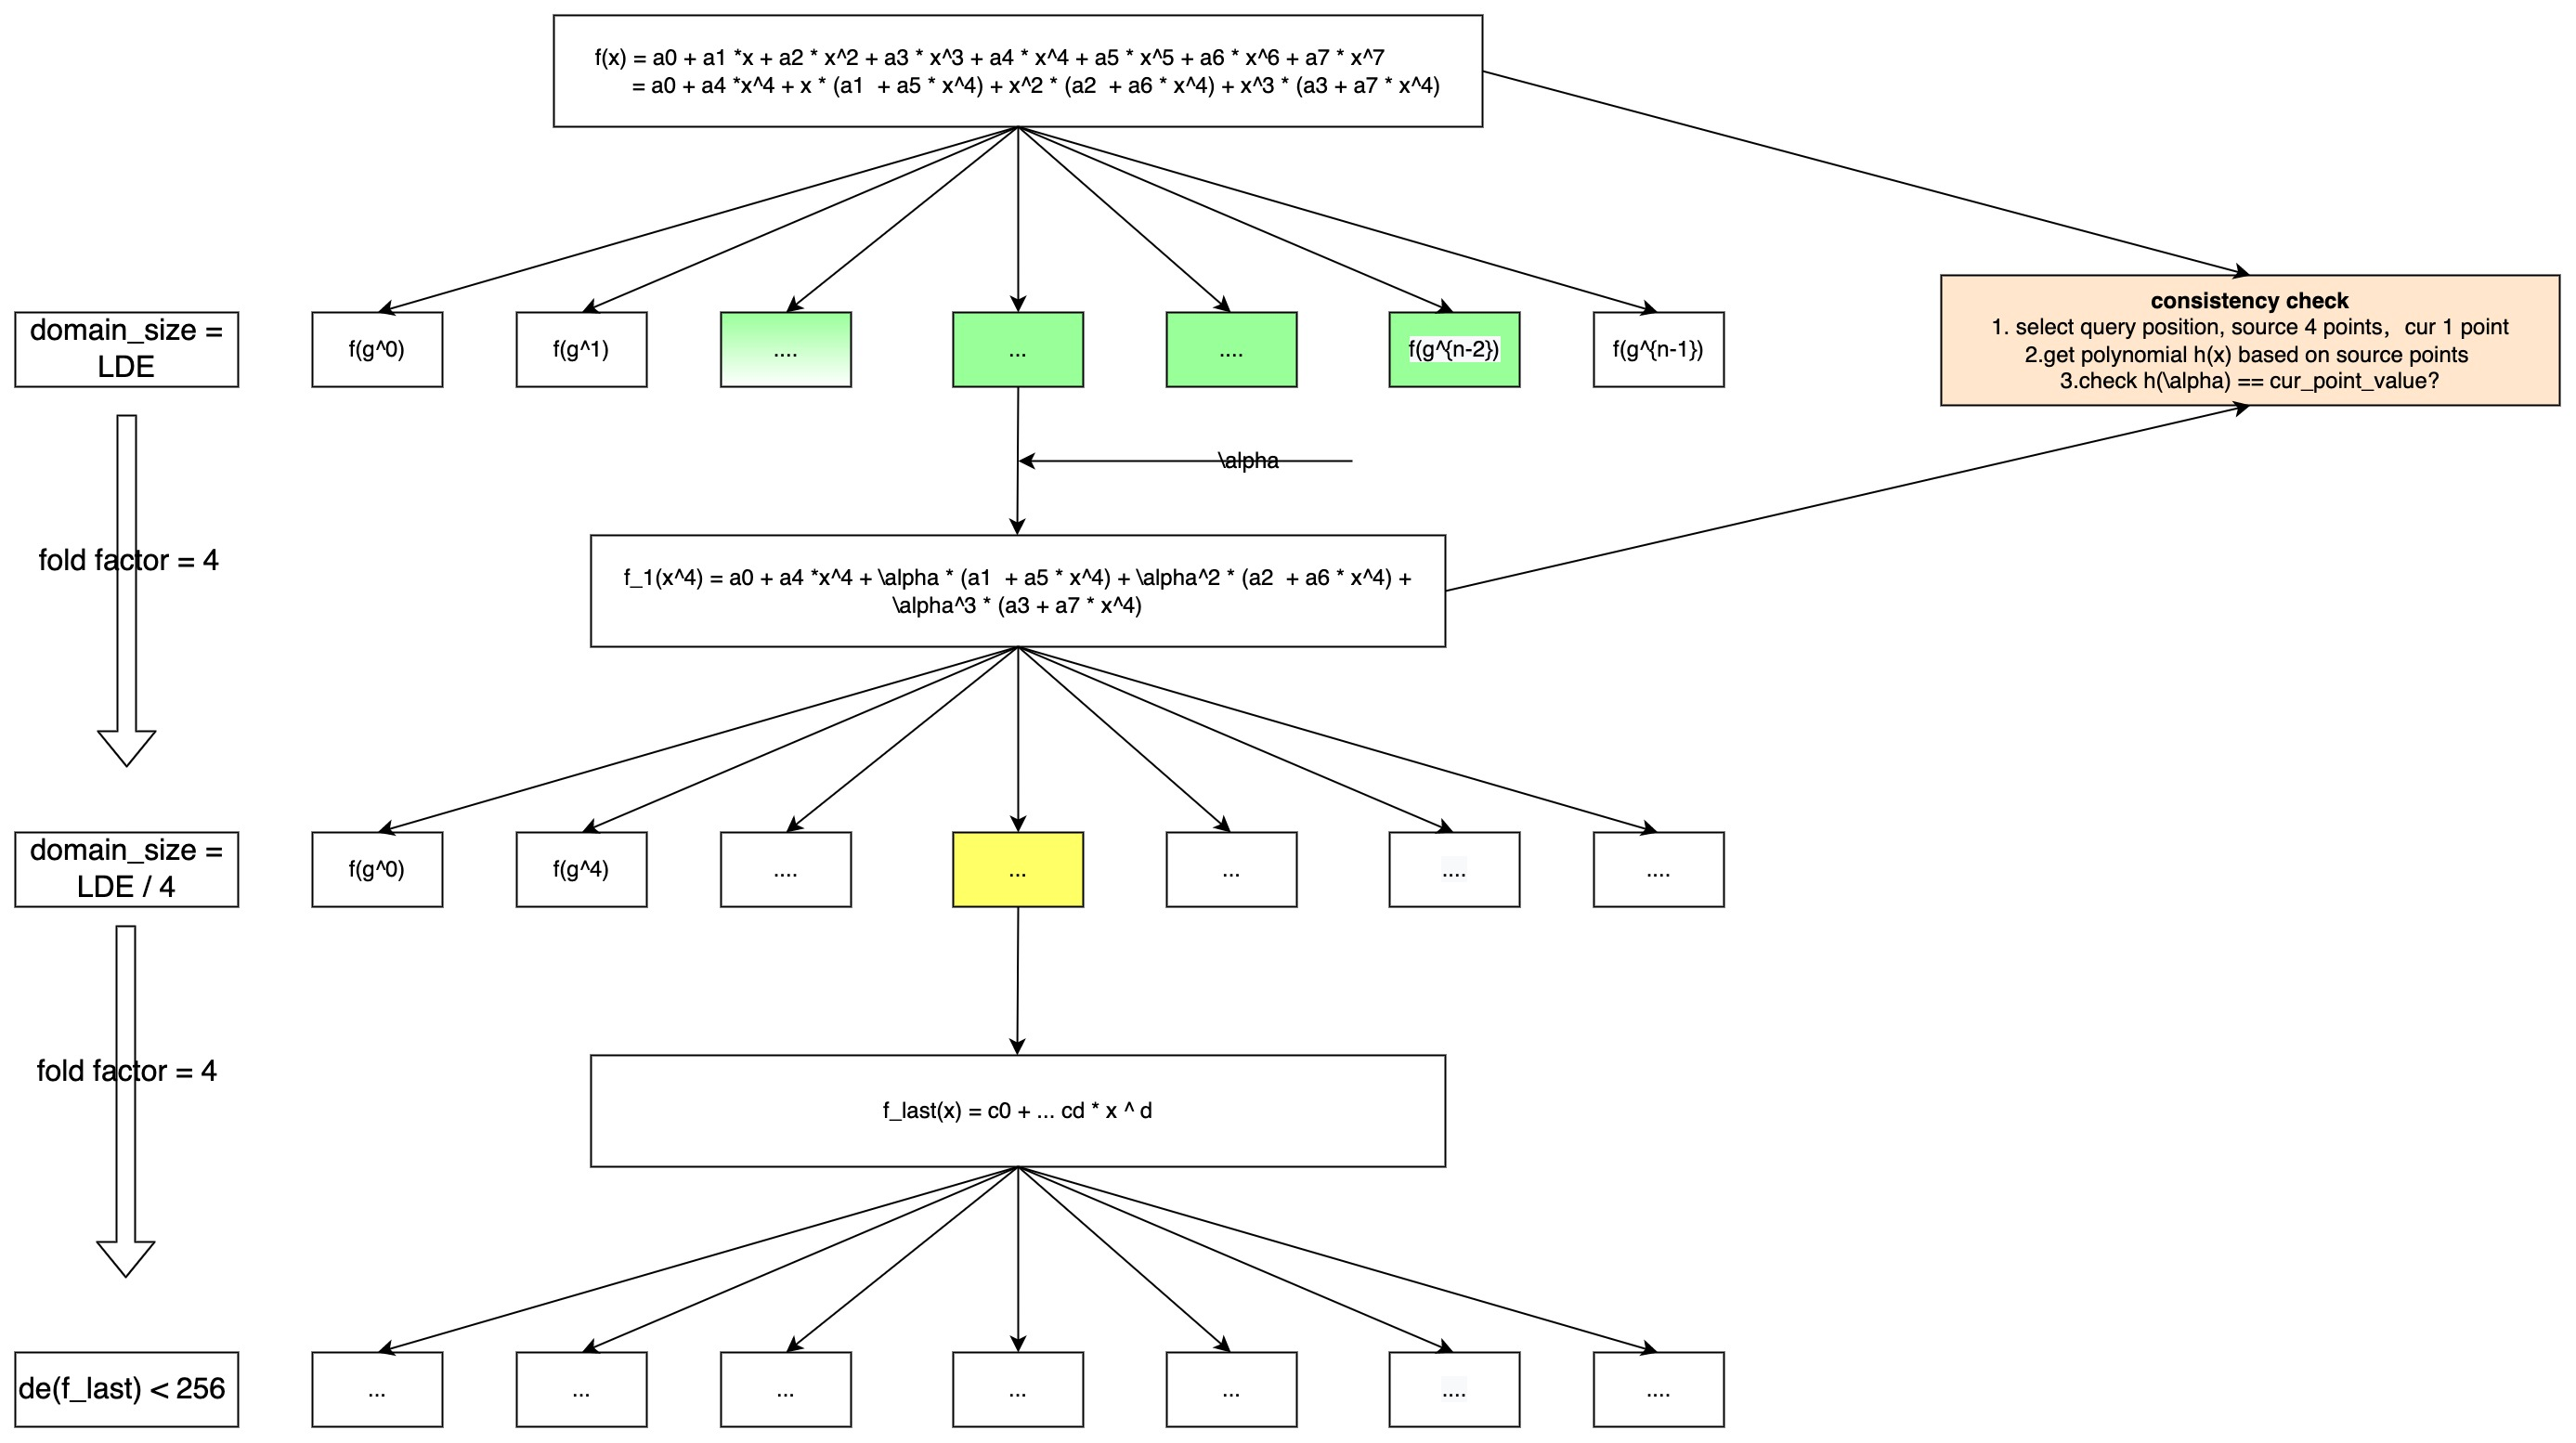
\includegraphics[width=0.8\textwidth]{fri.jpg}
    \caption{FRI protocol}
    \label{fig: FRI}
\end{figure}

FRI is a protocol that proves a committed polynomial having a bounded degree. Ola uses Deep-FRI for its polynomial commitment scheme. Figure \ref{fig: FRI} simply expresses the calculation process of FRI, anyone can read DEEP-FRI \cite{cryptoeprint:2019/336} for more details.
\subsubsection{Benchmark}\label{section: starky-benchmark}

Many optimizations have not yet been applied, and we expect to see more performance improvements as we devote more time to optimization. The benchmarks below should only be used as a rough guide to expected future performance.

In the benchmarks below, the VM executes the same Fibonacci calculator program for $2^{20}$ cycles at 100-bit target security level on an advanced 64-core CPU.

\begin{table}[!ht]
    \centering
    \begin{tabular}{|r|r|r|r|r|}
        \hline
        VM cycles & Execution time & Proving time & RAM consumption & Proof size \\
        \hline
        $2^{18}$ & 81.115 ms & 2.932 s & 5.6 GB & 175 KB \\
        \hline
        $2^{19}$ & 159.80 ms & 6.143 s & 11.1 GB & 181 KB \\
        \hline
        $2^{20}$ & 318.08 ms &12.688 s & 23.2 GB & 187 KB \\
        \hline
        $2^{21}$ & 627.38 ms & 29.923 s & 45.3 GB & 195 KB \\
        \hline
        $2^{22}$ & 1240.4 ms & 61.834 s & 86.6 GB & 208 KB \\
        \hline
        $2^{23}$ & 2453.8 ms & 128.62 s & 176 GB & 216 KB \\
        \hline
    \end{tabular}
\end{table}


\subsection{Plonky2} \label{sec:Plonky2}

Plonky2 \cite{website:plonky2} = Plonkish contraints system + DEEP-FRI commitment + Goldilocks field. We plan to use Plonky2 as our recursive Layer2 and Layer3 (supported in the future) because it's more suitable for specific computation than Starky which is more suitable for ZKVM. It should be noted that the designs described in this are the original version of Plonky2, which will be more convenient to learn for the reader.

\subsubsection{Circuit config} \label{sec:circuit-config}

There some types of configure in plonky2, let we make some clarification on this first:
\begin{itemize}
    \item \verb|num_wires| is the maximum column number one row;
    \item \verb|routed_num_wires| is the maximum wires one row;
    \item \verb|num_constants| is the maximum constants one row; 
    \item \verb|use_base_arithmeric_gate| if the flag of base gate or extension gate;
    \item \verb|security_bit| is the security level of prove system;
    \item \verb|num_challenges| is the security parameter to get security\_bit level;
    \item \verb|zero_knowledge| is the flag of blind;
    \item \verb|max_quotient_degree_factor| is the order parameter of constraint; 
    \item \verb|rate_bits| is the extension parameters for domain extension
    \item \verb|cap_height| is the special parameter of merkle tree;
    \item \verb|proof_of_work_bit| is the hardness parameter of query points;
    \item \verb|reduction_strategy| id the parameters of Fri-reduction;
\end{itemize}  

\paragraph{standard-recursion-config}

\hspace*{\fill} \\
\begin{lstlisting}[language=rust]
pub fn standard_recursion_config() -> Self {
    Self {
        num_wires: 135,
        num_routed_wires: 80,
        num_constants: 2,
        use_base_arithmetic_gate: true,
        security_bits: 100,
        num_challenges: 2,
        zero_knowledge: {\color{green}false},
        max_quotient_degree_factor: 8,
        fri_config: FriConfig {
            rate_bits: 3,
            cap_height: 4,
            proof_of_work_bits: 16,
            reduction_strategy: FriReductionStrategy::ConstantArityBits(4, 5),
            num_query_rounds: 28,
        },
    }
}  
\end{lstlisting}

\paragraph{standard-recursion-zk-config}

\hspace*{\fill} \\
\begin{lstlisting}[language=rust]
pub fn standard-recursion-zk-config() -> Self {
    Self {
        num_wires: 135,
        num_routed_wires: 80,
        num_constants: 2,
        use_base_arithmetic_gate: true,
        security_bits: 100,
        num_challenges: 2,
        zero_knowledge: {\color{green}true},
        max_quotient_degree_factor: 8,
        fri_config: FriConfig {
            rate_bits: 3,
            cap_height: 4,
            proof_of_work_bits: 16,
            reduction_strategy: FriReductionStrategy::ConstantArityBits(4, 5),
            num_query_rounds: 28,
        },
    }
}
\end{lstlisting}
  
\subsubsubsection{standard-ecc-config}

\hspace*{\fill} \\
\begin{lstlisting}[language=rust]
pub fn standard_ecc_config() -> Self {
    Self {
        num_wires: 136,
        num_routed_wires: 80,
        num_constants: 2,
        use_base_arithmetic_gate: true,
        security_bits: 100,
        num_challenges: 2,
        zero_knowledge: false,
        max_quotient_degree_factor: 8,
        fri_config: FriConfig {
            rate_bits: 3,
            cap_height: 4,
            proof_of_work_bits: 16,
            reduction_strategy: FriReductionStrategy::ConstantArityBits(4, 5),
            num_query_rounds: 28,
        },
    }
}   
\end{lstlisting}
  
\paragraph{wide-ecc-config}


\begin{lstlisting}[language=rust]
pub fn wide_ecc_config() -> Self {
    Self {
        num_wires: 234,
        num_routed_wires: 80,
        num_constants: 2,
        use_base_arithmetic_gate: true,
        security_bits: 100,
        num_challenges: 2,
        zero_knowledge: false,
        max_quotient_degree_factor: 8,
        fri_config: FriConfig {
            rate_bits: 3,
            cap_height: 4,
            proof_of_work_bits: 16,
            reduction_strategy: FriReductionStrategy::ConstantArityBits(4, 5),
            num_query_rounds: 28,
        },
    }
} 
\end{lstlisting}
 

\subsubsection{Gates} \label{sec:gates}

Each gate is a row with 135 columns. As different custom gate has different complexity, for some complex gate 135 columns may only constrain one
operation while for other simple gates, 135 columns may constrain several operations. The index of operation in a row is called a slot index.

Steps to using a custom gate:
\begin{itemize}
    \item Ensure the type of gate;
    \item Ensure the row and slot location of the gate;
    \item Ensure the wires layout of the gate;
    \item Ensure the consistency between public data and wires of gate;
    \item Ensure the row location of public data;\
    \item Finalize the trace table;
    \item Constraint for trace table;
    \item Generate proof;
\end{itemize}

For the convenience of description, the trace tables in this paper only show one operation which is slot 0.
\subsubsubsection{Custom gates}
\paragraph{arithmetic\_base}

ArithmeticGate is a gate which can perform a weighted multiply-add, i.e.
\[ \text{res} = \text{cons\_0} \times \text{mul\_0} \times \text{mul\_1} + \text{cons\_1} \times \text{add}. \]

The structure of gate is shown in \figref{fig:arithmetic-gate}.

\begin{figure}[!ht]
    \centering
    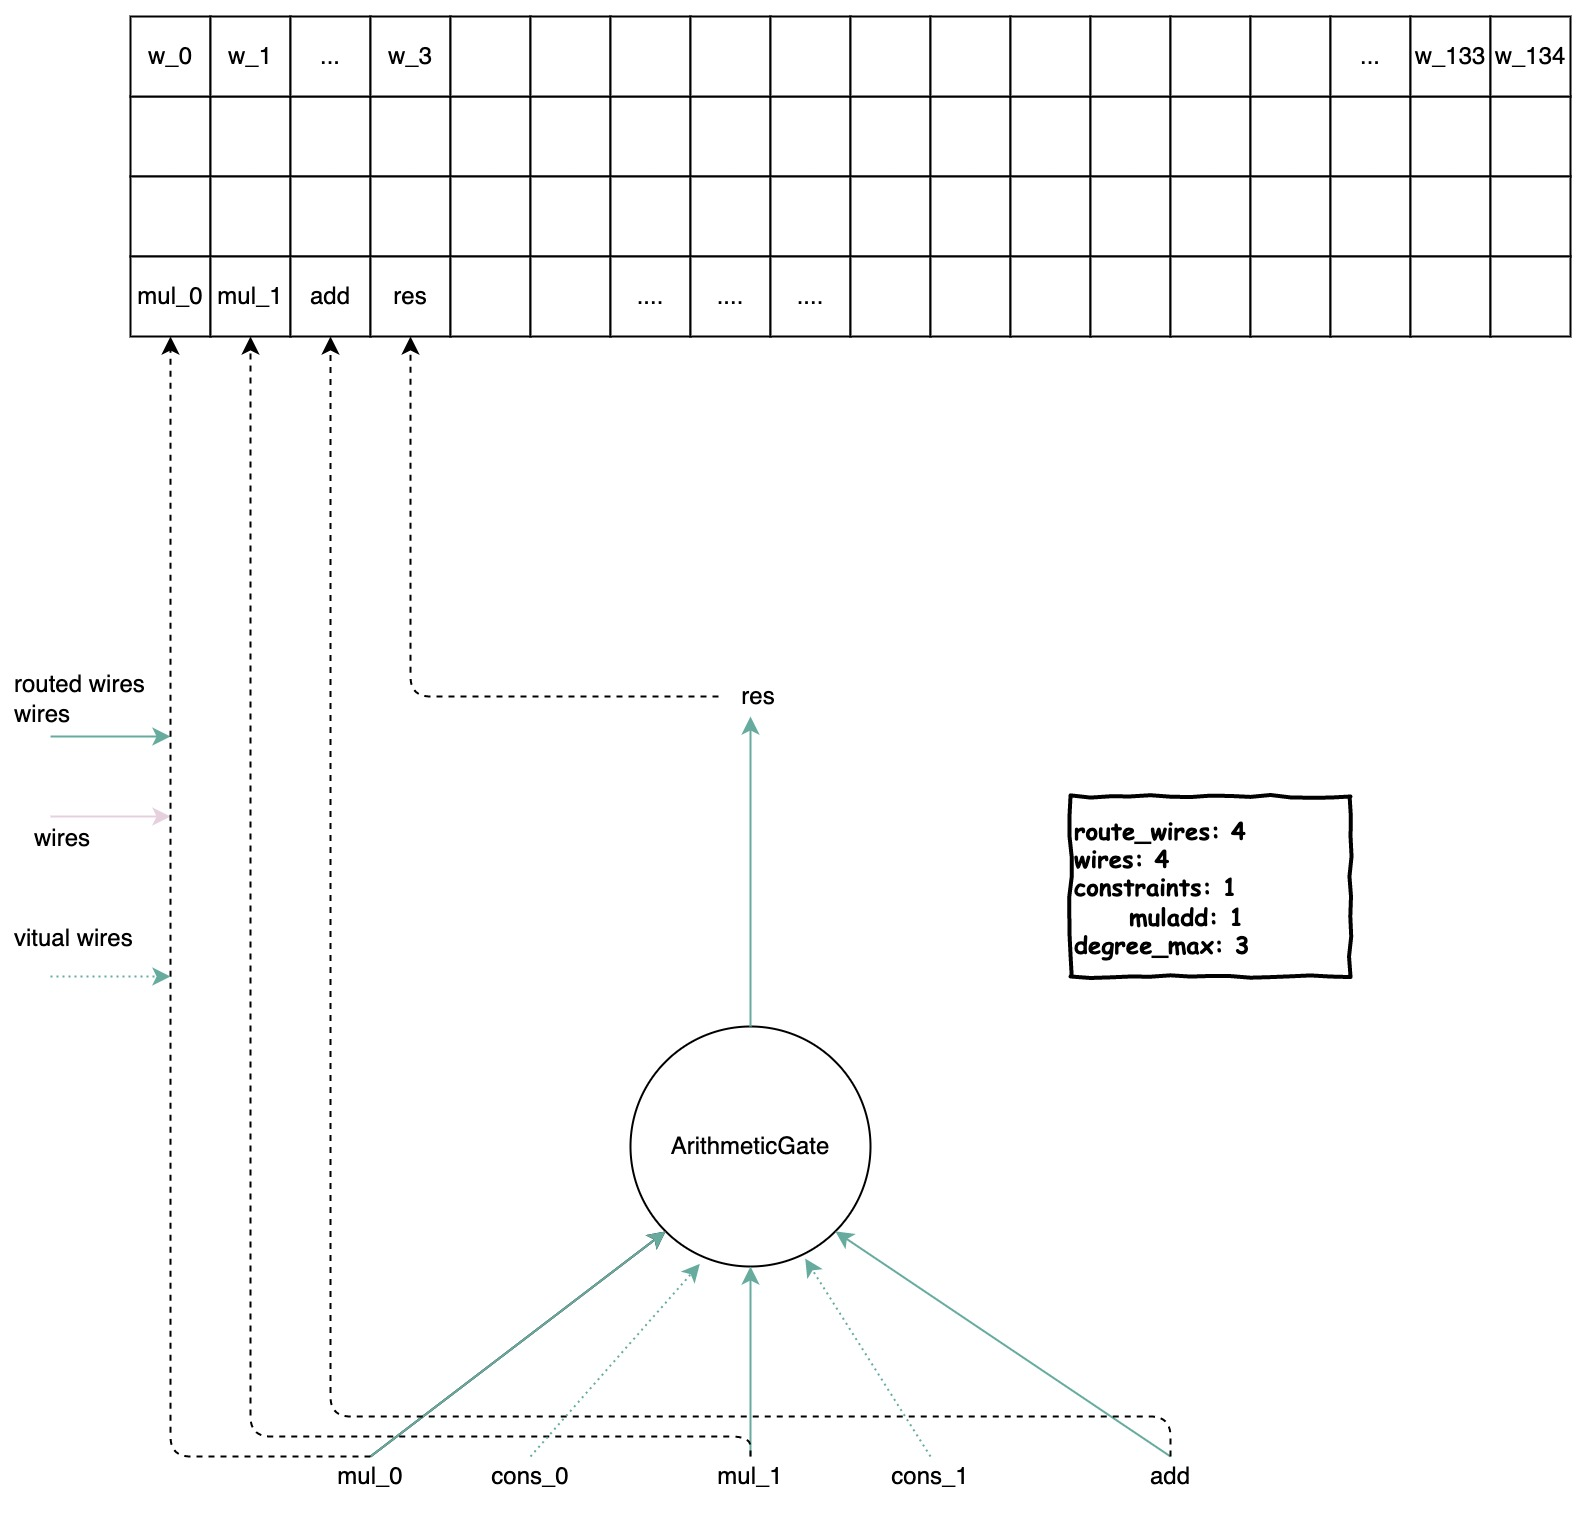
\includegraphics[width=0.5\textwidth]{gates/arithmetic_base.jpeg}
    \caption{ArithmeticGate}
    \label{fig:arithmetic-gate}
\end{figure}

There's only one constraint per operation, and degree is 3.

\subsubsubsection{arithmetic\_extension}

\hspace*{\fill}

\indent To understand the design principle of this Gate, we must first understand \href{https://en.wikipedia.org/wiki/Field_extension#Extension_field}{Field extension}. 

Taking Plonky2's Goldilocks field as an example, we give the extension field elements under quadratic, quartic, and quintic extensions respectively in \ref{fig:goldilocks field extension}.

\begin{figure}[!ht]
    \centering
    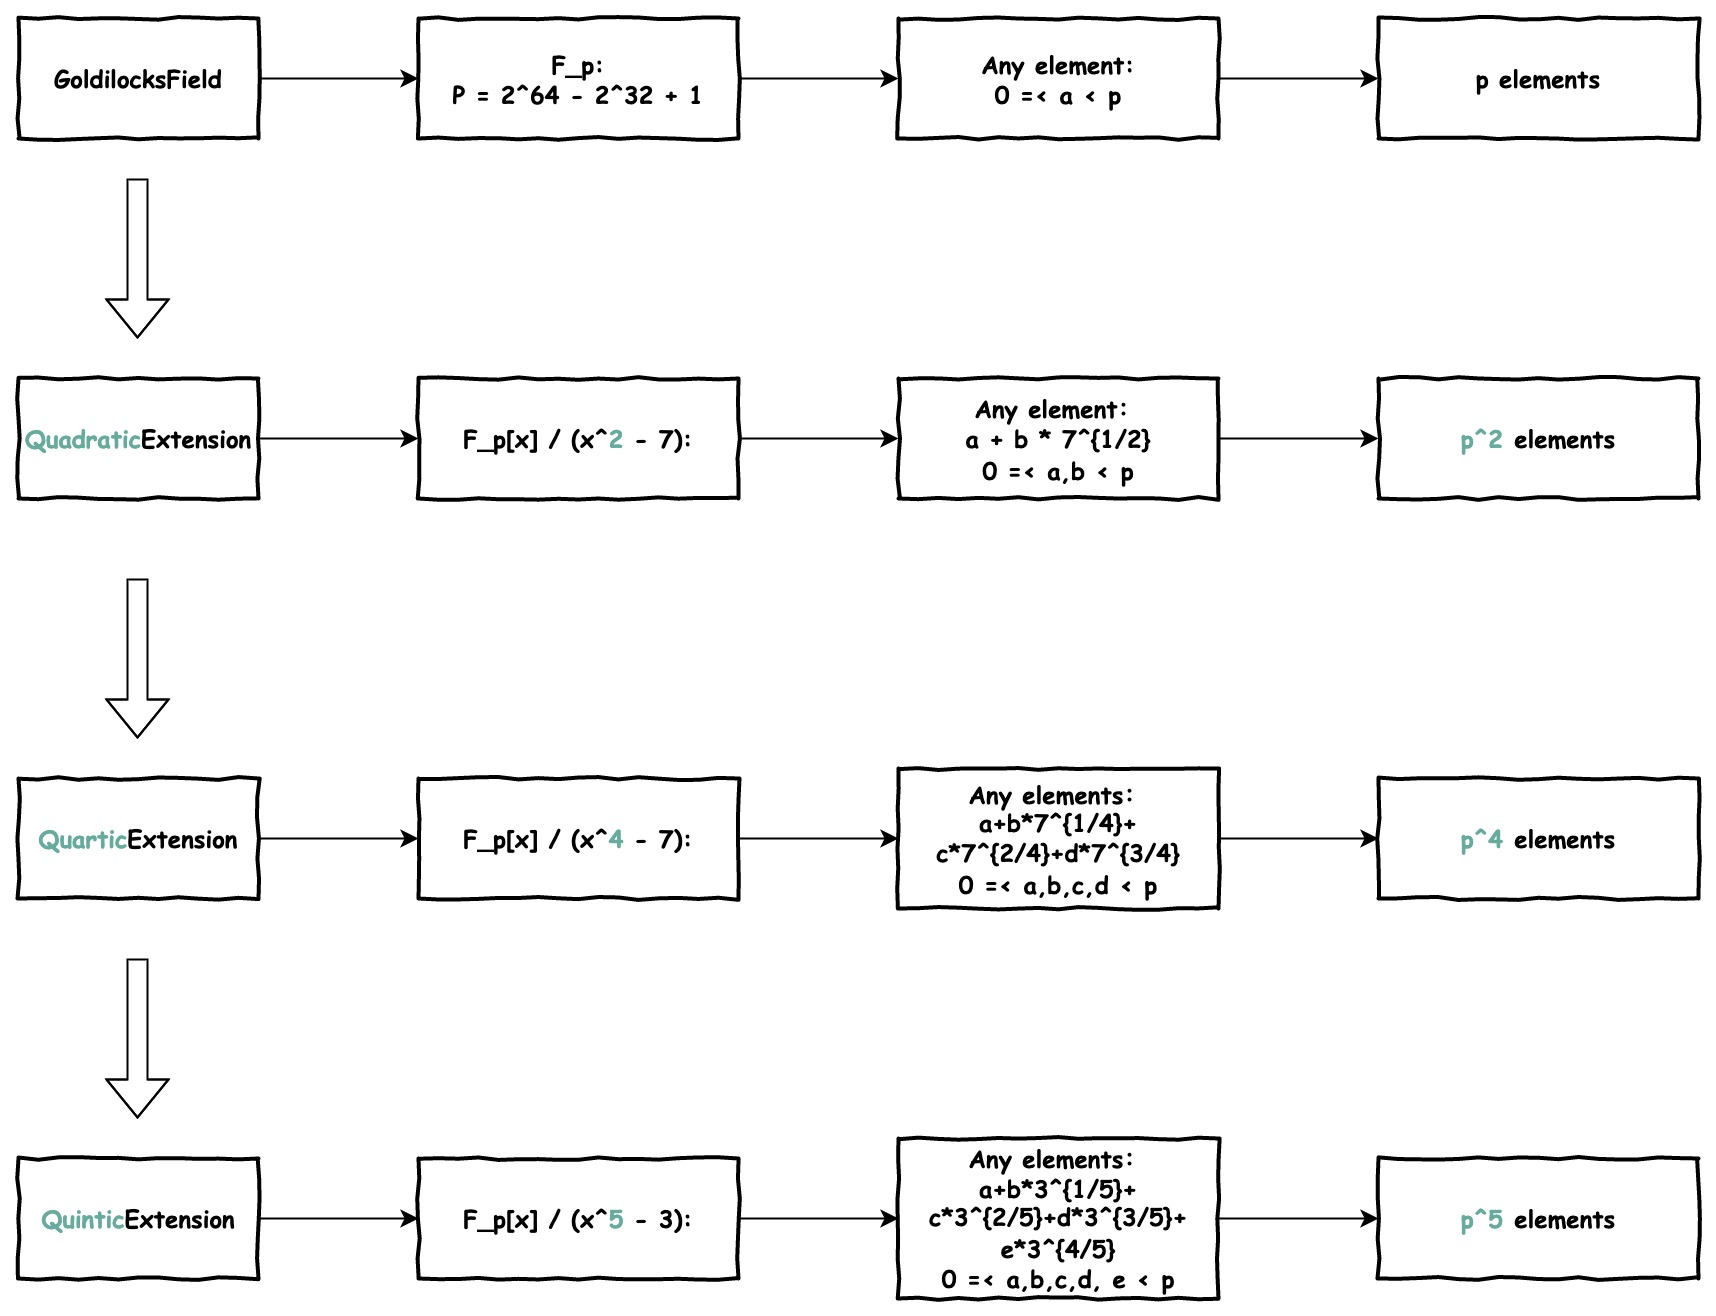
\includegraphics[width=0.6\textwidth]{gates/arthmetic_extension_ext.jpeg}
    \caption{Goldilocks Field Extension}
    \label{fig:goldilocks field extension}
\end{figure}

It is easy to see that for QuadraticExtension Field, the elements on its domain take the form $a+b\sqrt{7}, \ a,b \in F_p$.
It can be seen that on the quadratic extension domain, there are $p^2$ elements and the original domain is a subset of the quadratic extension domain.

ArithmeticExtensionGate is also a gate that can perform a weighted multiply-add, i.e.
\[ \text{res} = \text{cons\_0} \times \text{mul\_0} \times \text{mul\_1} + \text{cons\_1} \times \text{add} \]

The elements of the QuadraticExtension Field are represented in the form $[a, b]$, so the Gate design for arithmetic\_extension has the following form:

The structure of the gate is shown in \ref{fig:arthmetic-extension}. There's only one constraint per operation, and the degree is 3.
\begin{figure}[!ht]
    \centering
    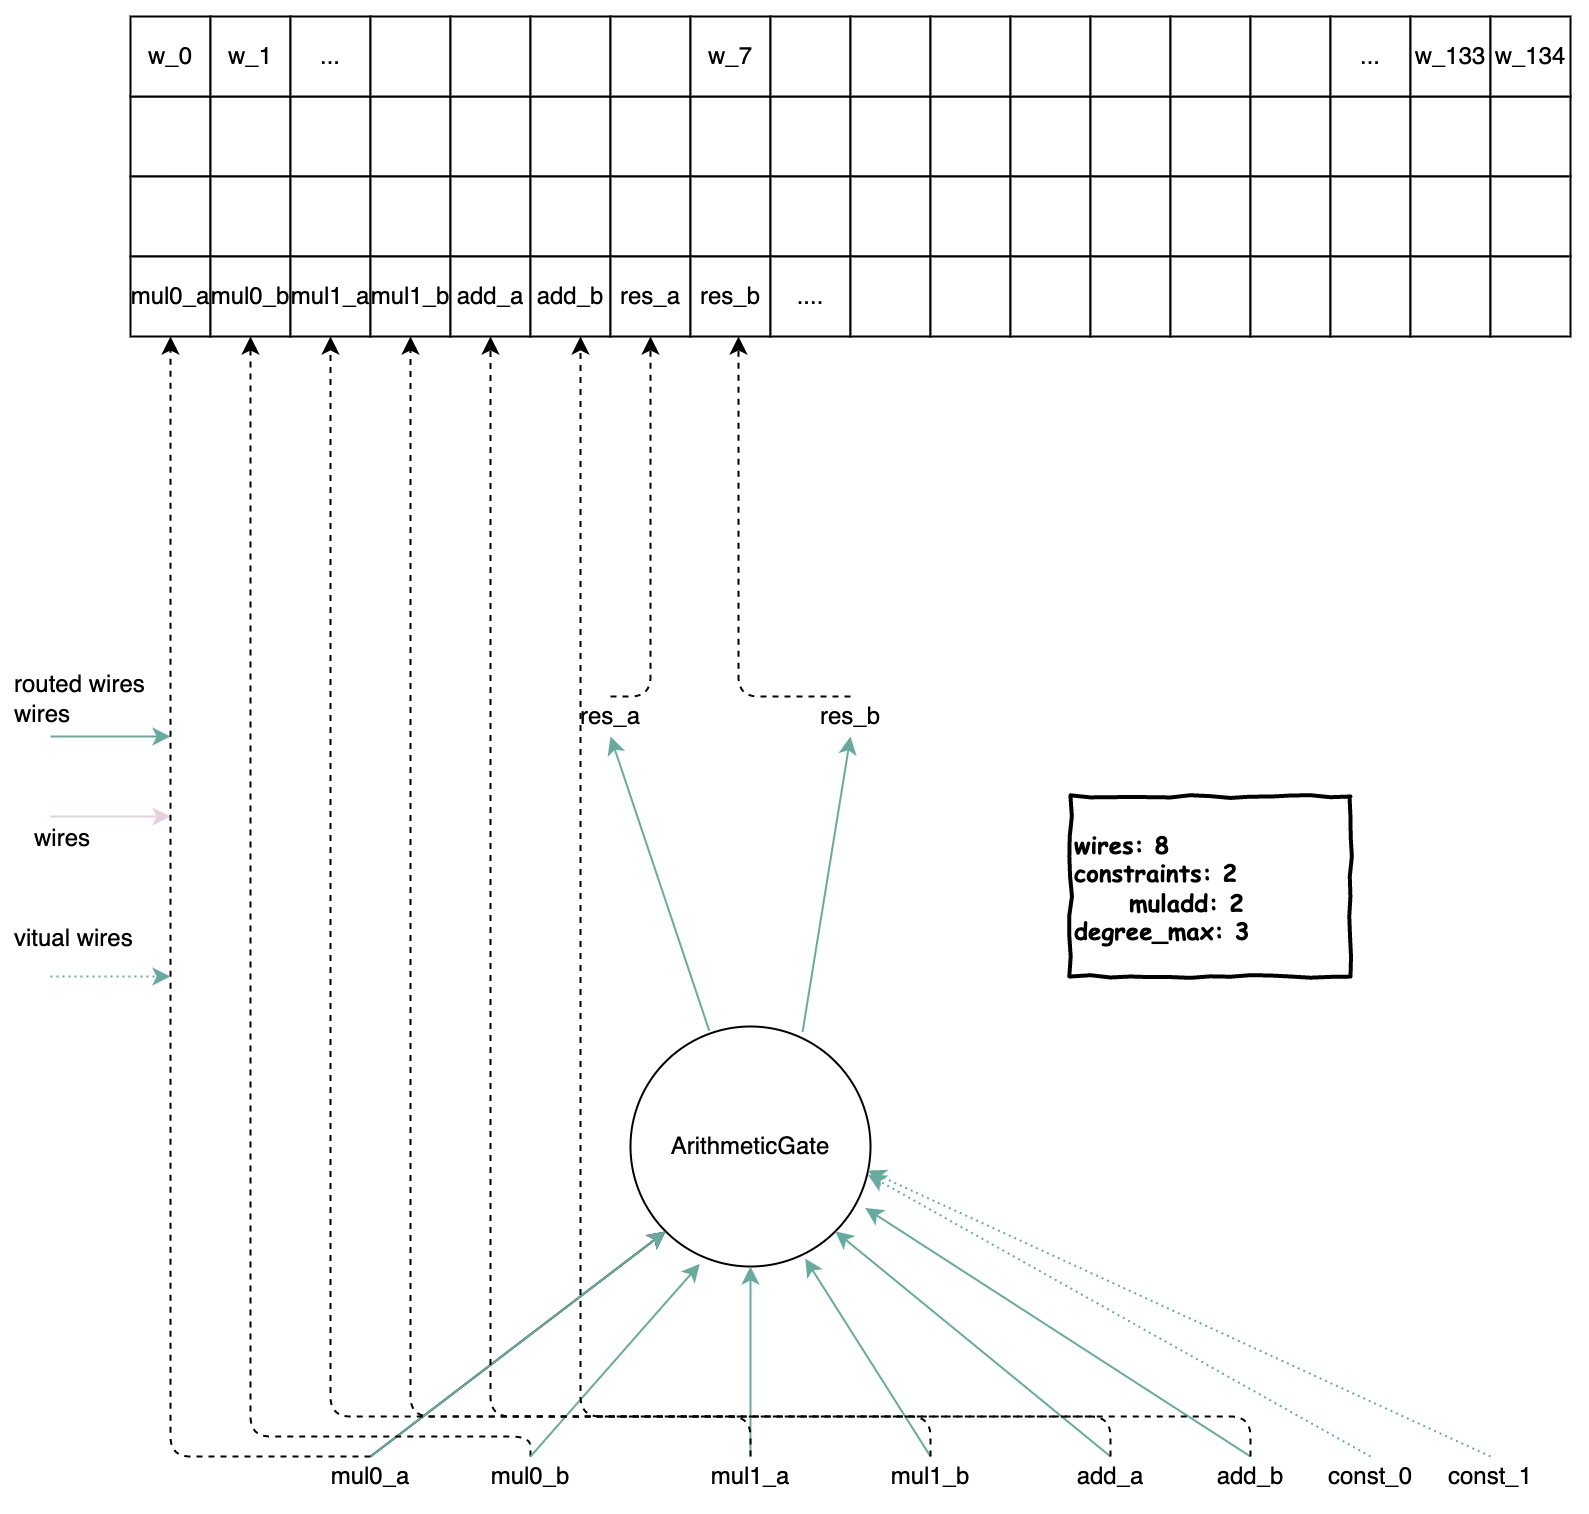
\includegraphics[width=0.6\textwidth]{gates/arthmetic_extension.jpeg}
    \caption{ArithmeticExtensionGate}
    \label{fig:arthmetic-extension}
\end{figure}
\paragraph{base\_sum}

BaseSumGate is used to constrain the input to be composed of limbs which are arranged in little-endian. There are two kinds of constraints:

For each limb, limb is in range $[0, \text{base})$:
\[ \sum_{i=0}^{\text{base}}(\text{limb}_i - i) = 0. \]

Input is composed of limbs:
\[ \text{input} = \sum_{i=0}^{n-1} \text{limb}_{n-1-i} \times \text{base}^i. \]

The structure of gate is shown in \figref{fig:base-sum}.
\begin{figure}[!ht]
    \centering
    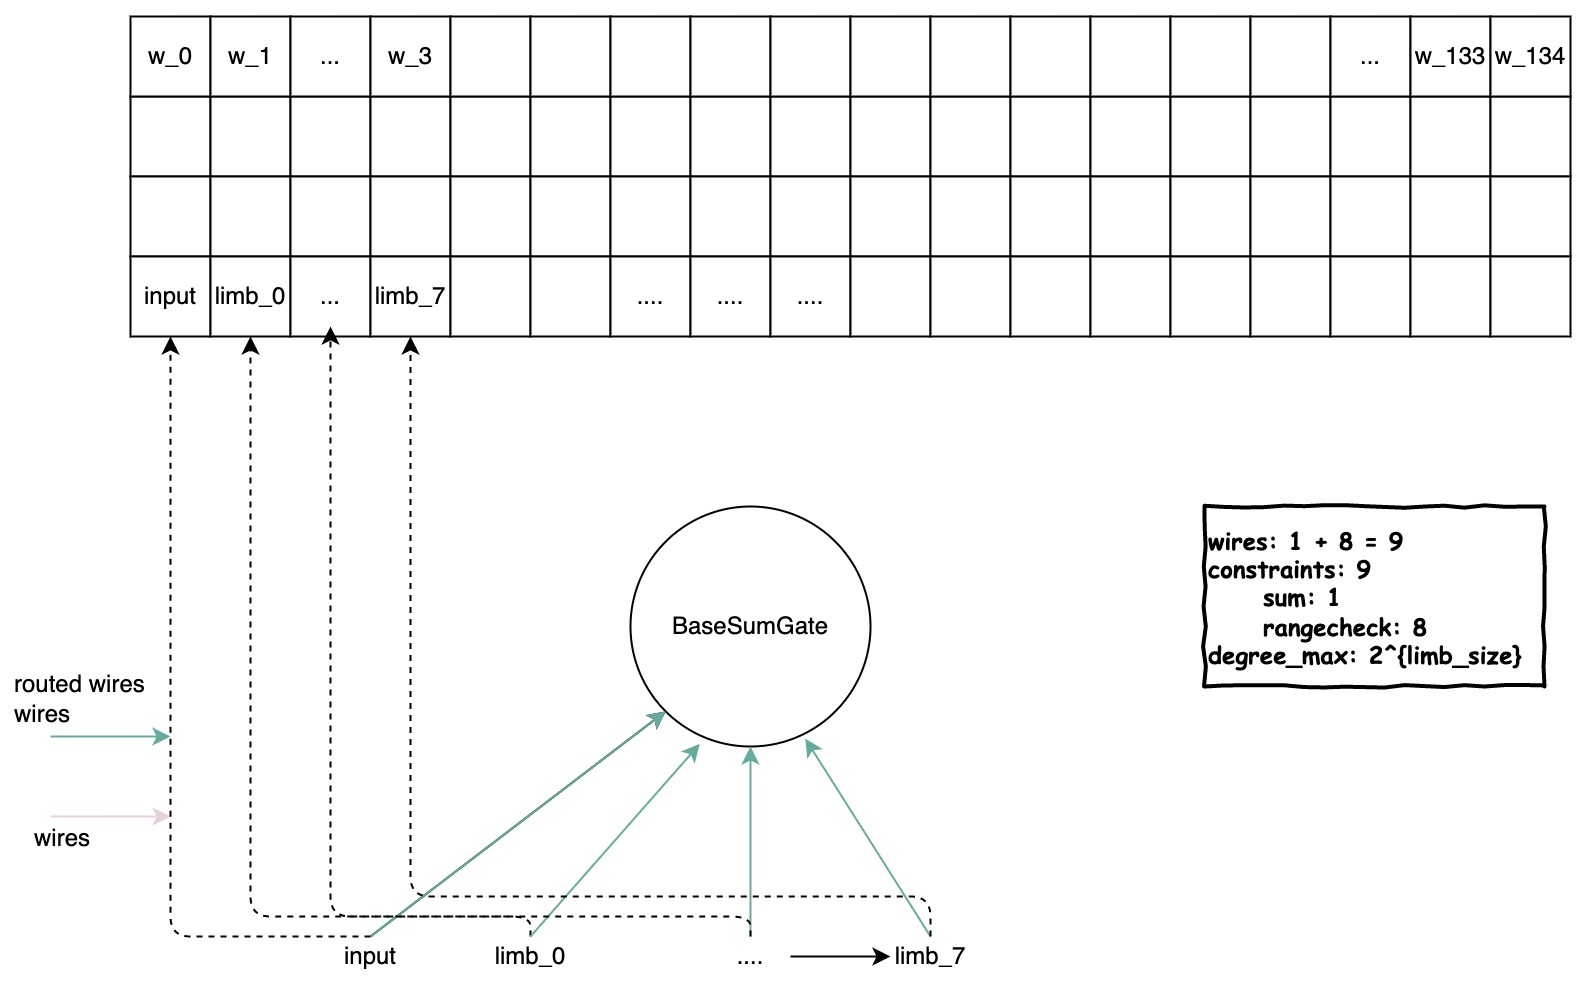
\includegraphics[width=0.8\textwidth]{gates/base_sum.jpeg}
    \caption{BaseSumGate}
    \label{fig:base-sum}
\end{figure}

There's 1 constraint for sum check and 8 constraints for limbs' range check. Degree of the gate is $2^{\text{limb\_size}}$ happens when limbs' range check.

\subsubsubsection{exponentiation}

\hspace*{\fill}

\indent ExponentiationGate is a gate for raising a value to a power. The trace table contains the base, bits of the exponent, output, and intermediate value of the bits.

Take $A^{21} = A^{10101_b}$ for example to describe intermediate value, the bits are [1, 0, 1, 0, 1].

\begin{enumerate}
    \item Current bit = 1, we start from 1, and times $A^{bit}$ we get $A$
    \item Current bit = 0,
    \begin{itemize}
        \item Square prev\_intermediate\_value $A^{1_b << 1} = A^{10_b}$
        \item Then times $A^{bit}$ we get $A^{10_b} \times A^0 = A^{10_b}$
    \end{itemize}
    \item Current bit = 1,
    \begin{itemize}
        \item Square prev\_intermediate\_value $A^{10_b << 1} = A^{100_b}$
        \item Then times $A^{bit}$ we get $A^{100_b} \times A = A^{101_b}$
    \end{itemize}
    \item Current bit = 0,
    \begin{itemize}
        \item Square prev\_intermediate\_value $A^{101_b << 1} = A^{1010_b}$
        \item Then times $A^{bit}$ we get $A^{1010_b} \times 1 = A^{1010_b}$
    \end{itemize}
    \item Current bit = 1,
    \begin{itemize}
        \item Square prev\_intermediate\_value $A^{1010_b << 1} = A^{10100_b}$
        \item Then times $A^{bit}$ we get $A^{10100_b} \times A = A^{10101_b}$
    \end{itemize}
\end{enumerate}

And we get the last intermediate value $A^{10101_b}$ which should be equal to the output.

Let's take another example of a specific number $2^{13} = 2^{1101_b}$, and have a look at the trace cell:
\begin{center}
    \begin{tabular}{ |c|c|c|c|c|c|c|c|c|c| }
        \hline
        base & b\_0 & b\_1 & b\_2 & b\_3 & output & inter\_0 & inter\_1 & inter\_2 & inter\_3 \\
        \hline
        2 & 1 & 0 & 1 & 1 & 8192 & 2 & 8 & 64 & 8192 \\
        \hline
    \end{tabular}
\end{center}

The structure of the gate is shown in \ref{fig:exponetiation-gate}.
\begin{figure}[!ht]
    \centering
    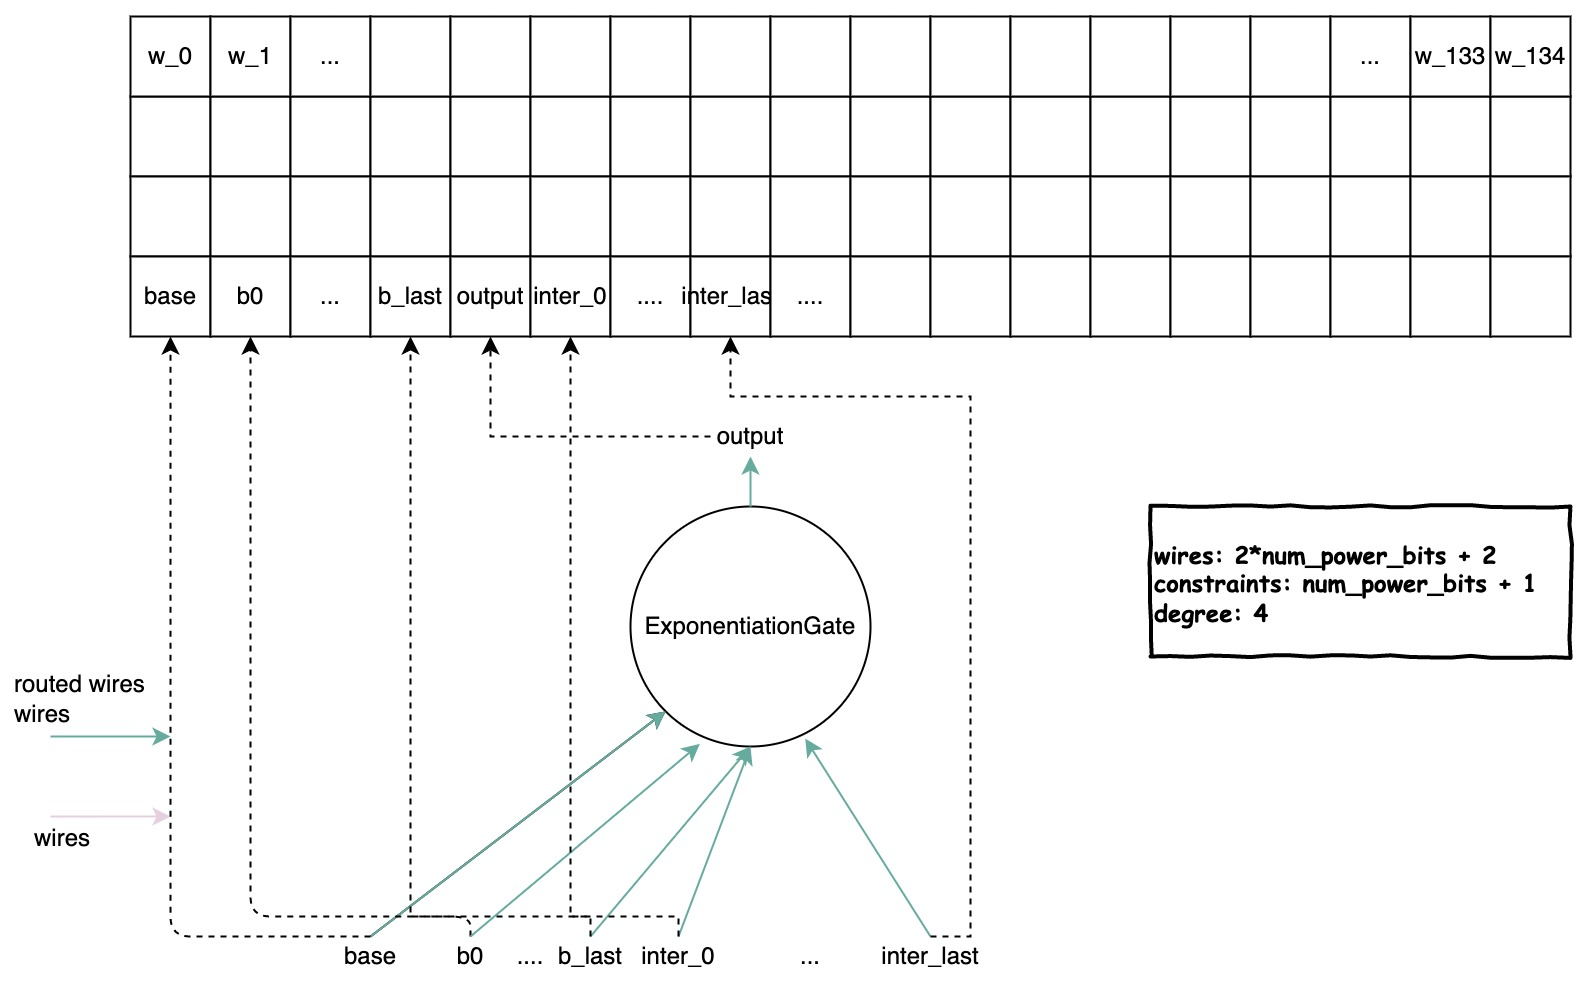
\includegraphics[width=0.6\textwidth]{gates/exponentiation.jpeg}
    \caption{ExponentiationGate}
    \label{fig:exponetiation-gate}
\end{figure}

Each step result is constrainted with intermediate values, and output is constrained with the final intermediated value, a total of $bits + 1$ constraints.
The degree of the gate is 4, which is determined by the intermediate calculation:
\begin{lstlisting}[language=rust]
let computed_intermediate_value =
            prev_intermediate_value * (cur_bit * base + not_cur_bit);
\end{lstlisting}

\paragraph{poseidon}

\href{https://www.poseidon-hash.info/}{Poseidon} is a hash function designed for the Zero-Knowledge proof system.
Its calculation process is rough as follows:

\begin{figure}[!ht]
    \centering
    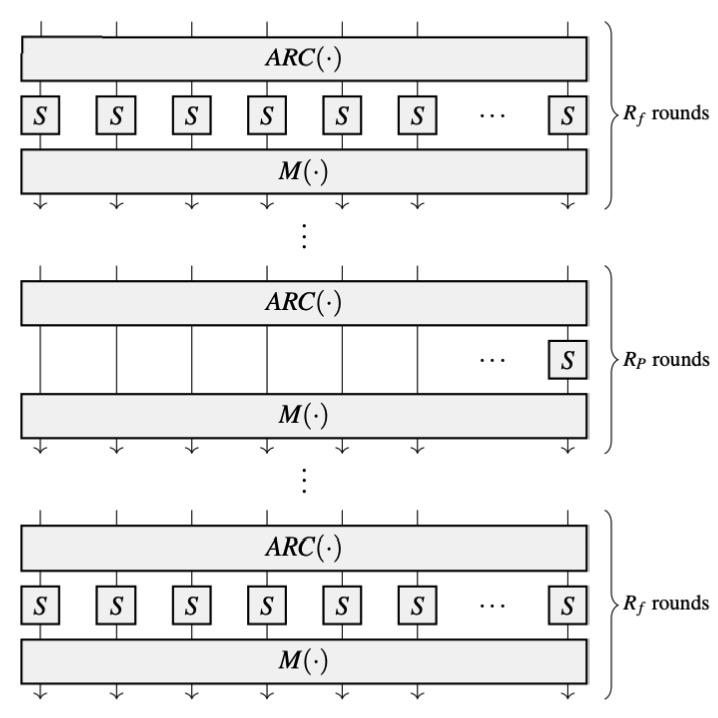
\includegraphics[width=0.6\textwidth]{gates/poseidon_process.jpeg}
    \caption{Construction of poseidon}
    \label{fig:poseidon-process}
\end{figure}

Each round function of Poseidon permutation consists of the following three components.
\begin{enumerate}
    \item ARC(.): AddRoundConstants
    \item S: SubWords
    \item M(.): MixLayer
\end{enumerate}

The Trace of the gate is like this:
\begin{figure}[!ht]
    \centering
    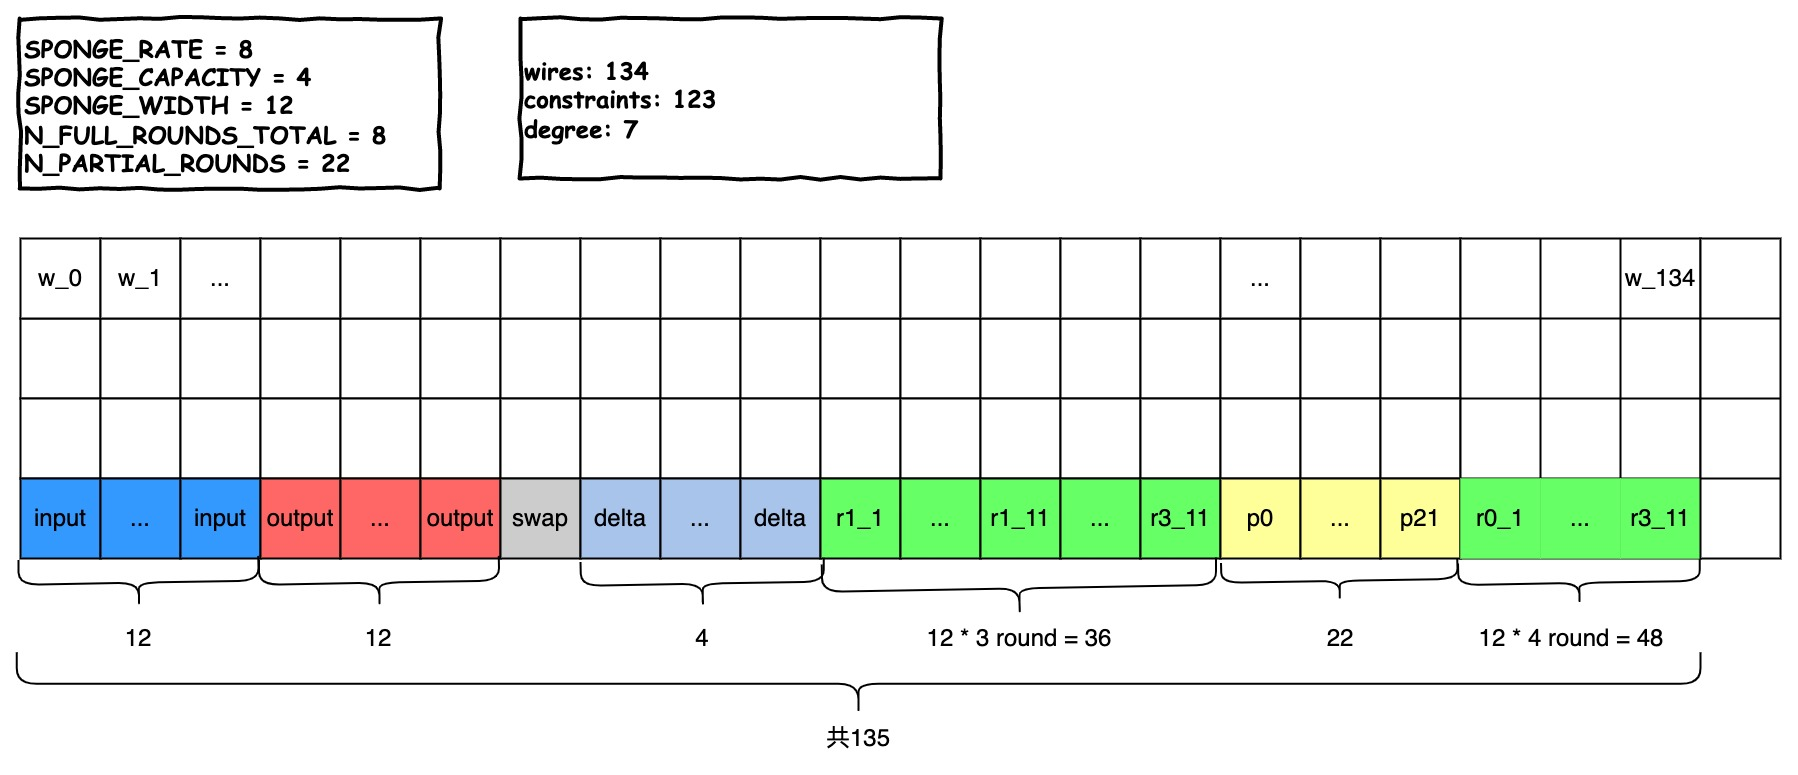
\includegraphics[width=0.6\textwidth]{gates/poseidon.jpeg}
    \caption{PoseidonGate}
    \label{fig:poseidon-gate}
\end{figure}

\begin{itemize}
    \item input: components of the input, 12 elements.
    \item output: components of the output, 12 elements.
    \item swap: 0 or 1, Indicates whether the first four elements of the input are swapped with the last four elements.
    \item delta: used when swap is 1, $\text{delta}_i = \text{swap} \times (\text{input}_{\text{rhs}} - \text{input}_{\text{lhs}})$.
    \item green region: full rounds, ri\_1~ri\_11 is the state of each round.
    \item yellow region: partial rounds, each element is state[0] of each round.
\end{itemize}

Calculation process and related constraints:
\begin{itemize}
    \item Assert that swap is binary. (1 constraint)
    \begin{lstlisting}[language=rust]
constraints.push(swap * (swap - F::Extension::ONE))
    \end{lstlisting}
    \item Assert $\text{delta}_i = \text{swap} \times (\text{rhs} - \text{lhs})$. (4 constraints)
    \begin{lstlisting}[language=rust]
for i in 0..4 {
    ....
    constraints.push(swap * (input_rhs - input_lhs) - delta_i);
}
    \end{lstlisting}
    \item Initialize state: when swap=0, state=input; when swap=1, state is swapped input:
    \begin{figure}[!ht]
        \centering
        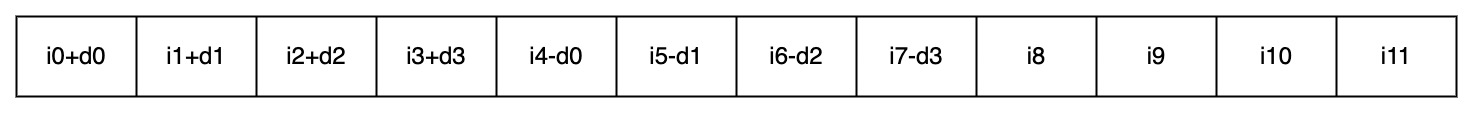
\includegraphics[width=0.6\textwidth]{gates/poseidon_state_init.jpeg}
        \caption{Poseidon State Init}
        \label{fig:poseidon-state-init}
    \end{figure}
    \begin{lstlisting}[language=rust]
for i in 0..4 {
    ...
    state[i] = vars.local_wires[input_lhs] + delta_i;
    state[i + 4] = vars.local_wires[input_rhs] - delta_i;
}
for i in 8..SPONGE_WIDTH {
    state[i] = vars.local_wires[Self::wire_input(i)];
}
    \end{lstlisting}
    \item Begin first full rounds calculation, for each round r (which is 0--3):
    \begin{itemize}
        \item Perform ARC: Add each element of state to the pre-generated value at a particular position in the array.
        \begin{lstlisting}[language=rust]
for i in 0..WIDTH {
    state[i] += F::from_canonical_u64(ALL_ROUND_CONSTANTS[i + WIDTH * round_ctr]);
}
        \end{lstlisting}
        \item Except for r=0, constrain each element of the state calculated in the previous round (the green part of the first slice of the figure). 
        (12 constraints per round, a total of 36 constraints)
        \item Perform SubWords: Turn state element by element x into $x \mapsto x^7$
        \item Perform MixLayer: Each element of the state is updated according to itself and a pre-generated array.
        \begin{lstlisting}[language=rust]
// r is the index of state elements here.
let mut res = F::ZERO;
    for i in 0..WIDTH {
    res += v[(i + r) % WIDTH] * F::from_canonical_u64(Self::MDS_MATRIX_CIRC[i]);
}
res += v[r] * F::from_canonical_u64(Self::MDS_MATRIX_DIAG[r]);
        \end{lstlisting}
    \end{itemize}
    \item Perform partial rounds:
    \begin{itemize}
        \item Perform ARC
        \begin{lstlisting}[language=rust]
for i in 0..12 {
    if i < WIDTH {
        state[i] += F::from_canonical_u64(Self::FAST_PARTIAL_FIRST_ROUND_CONSTANT[i]);
    }
}
        \end{lstlisting}
        \item Processing of state with $11 \times 11$ MDS (maximum distance separable) matrix.
        \begin{lstlisting}[language=rust]
result[0] = state[0];
for r in 1..12 {
    if r < WIDTH {
        for c in 1..12 {
            if c < WIDTH {
                let t = F::from_canonical_u64(
                    Self::FAST_PARTIAL_ROUND_INITIAL_MATRIX[r - 1][c - 1],
                );
                result[c] += state[r] * t;
            }
        }
    }
}
result
        \end{lstlisting}
        \item Perform 22 round sbox, for the first 21 rounds (r = 0--21):
        \begin{itemize}
            \item Take sbox\_in(yellow elements in the figure), and constrains state[0]=sbox\_in -- 21 rounds totally 21 constraints.
            \item \verb|state[0] = state[0]^7|
            \item \verb|state[0] += FAST_PARTIAL_ROUND_CONSTANTS[r]|
            \item Perform mds to state.
        \end{itemize}
        \item For the 22th round:
        \begin{itemize}
            \item \verb|state[0] = sbox_in| (i constraint)
            \item \verb|state[0] = state[0]^7|
            \item Perform mds to state.
        \end{itemize}
    \end{itemize}
    \item Perform second round "Full rounds", same with the first round. (the green part of the second slice of the figure). (12 constraints, 4 rounds totally of 48 constraints)
    \item Asserts computed result equals output. (12 constraints)
    \begin{lstlisting}[language=rust]
for i in 0..SPONGE_WIDTH {
    constraints.push(state[i] - vars.local_wires[Self::wire_output(i)]);
}
    \end{lstlisting}
\end{itemize}

The constraints of this gate in total is 123, the degree is 7 (when performing s-box, making $\text{state}[i] \mapsto \text{state}[i]^7$).

\paragraph{poseidon\_mds}

\hspace*{\fill}

\indent This gate is used for constraining outputs of Poseidon mds.

\begin{figure}[!ht]
    \centering
    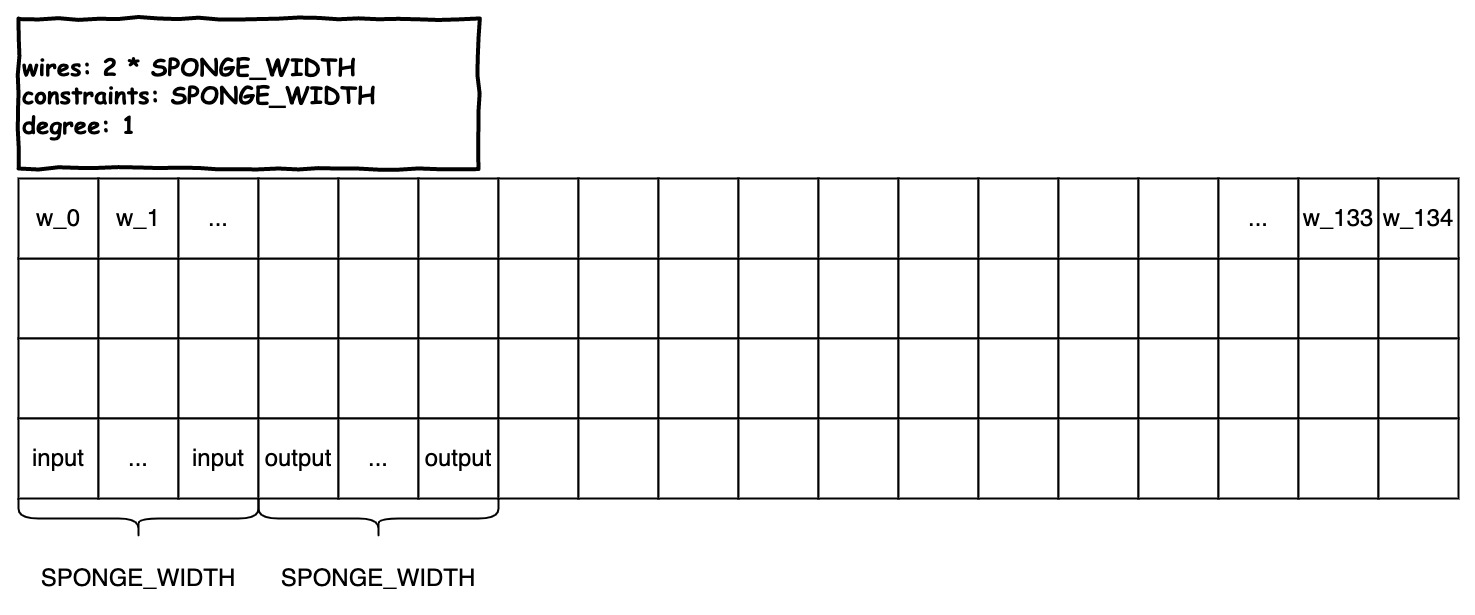
\includegraphics[width=0.6\textwidth]{gates/poseidon_mds.jpeg}
    \caption{PoseidonMdsGate}
    \label{fig:poseidon-mds}
\end{figure}

computed\_output is calculated from input, and constrained with output element by element, a total of 12 constraints (degree 1).
\begin{lstlisting}[language=rust]
let inputs: [_; SPONGE_WIDTH] = (0..SPONGE_WIDTH)
    .map(|i| vars.get_local_ext_algebra(Self::wires_input(i)))
    .collect::<Vec<_>>()
    .try_into()
    .unwrap();
let computed_outputs = Self::mds_layer_algebra(&inputs);
(0..SPONGE_WIDTH)
    .map(|i| vars.get_local_ext_algebra(Self::wires_output(i)))
    .zip(computed_outputs)
    .flat_map(|(out, computed_out)| (out - computed_out).to_basefield_array())
    .collect()
\end{lstlisting}

\paragraph{random\_access}

RandomAccessGate is used to verify that an element matches a value in the list.

\begin{figure}[!ht]
    \centering
    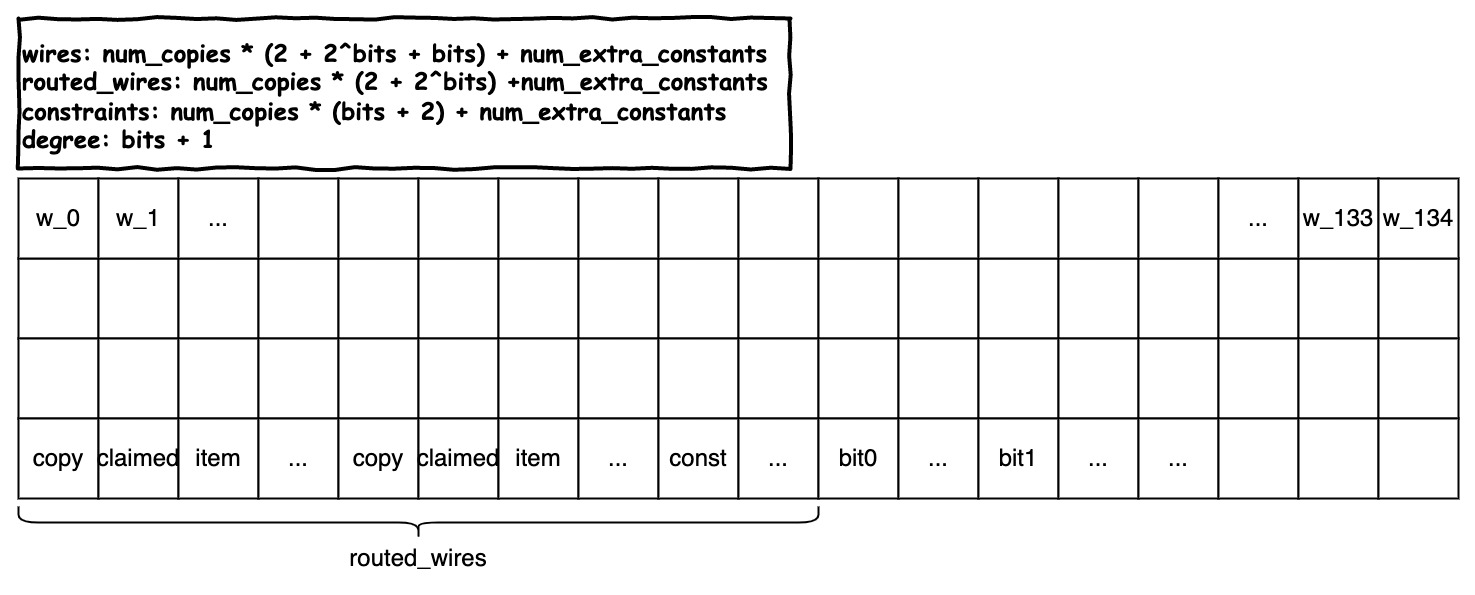
\includegraphics[width=0.6\textwidth]{gates/random_access.jpeg}
    \caption{RandomAccessGate}
    \label{fig:random-access}
\end{figure}

\begin{itemize}
    \item item: list items.
    \item copy: index of the target element in the list
    \item claimed: target element
    \item bit\_i: bits for the i-th copy
\end{itemize}

For each copy:
\begin{itemize}
    \item Constrain bits are 0 or 1. -- bits constraints for each copy, A total of num\_copied*bits constraints.
    \begin{lstlisting}[language=rust]
for &b in &bits {
    constraints.push(builder.mul_sub_extension(b, b, b));
}
    \end{lstlisting}
    \item Constraint copy consists of bits. -- 1 constraint for each copy, A total of num\_copied constraints.
    \begin{lstlisting}[language=rust]
let reconstructed_index = bits
    .iter()
    .rev()
    .fold(zero, |acc, &b| builder.mul_add_extension(acc, two, b));
constraints.push(builder.sub_extension(reconstructed_index, access_index));
    \end{lstlisting}
    \item For each bit, reconstruct items with a 2-elements-tuple, select the first element when the bit is 0, and select the second when the bit is 1.
    After the bits round, only one element remains, that is, the index element corresponding to bits, constraint it with claimed.
    \begin{figure}[!ht]
        \centering
        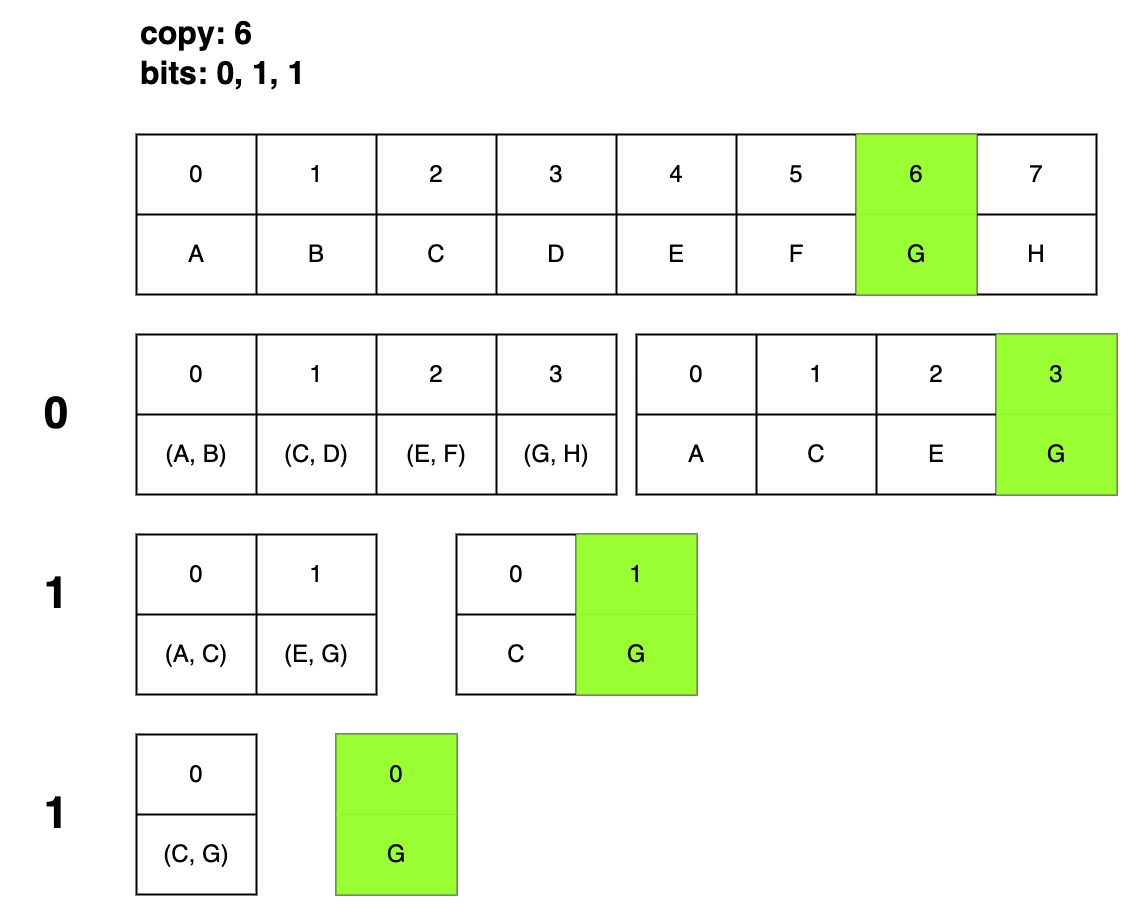
\includegraphics[width=0.6\textwidth]{gates/random_access_example.jpeg}
        \caption{Random Access Example}
        \label{fig:random-access-example}
    \end{figure}
    \begin{lstlisting}[language=rust]
for b in bits {
    list_items = list_items
        .iter()
        .tuples()
        .map(|(&x, &y)| builder.select_ext_generalized(b, y, x))
        .collect()
}
// Check that the one remaining element after the folding is the claimed element.
debug_assert_eq!(list_items.len(), 1);
constraints.push(builder.sub_extension(list_items[0], claimed_element));
    \end{lstlisting}
\end{itemize}

Finally, the constant is constrained -- A total of num\_extra\_constraints constraints.

In summary, there're $\text{num\_copies} \times (\text{bits} + 2) + \text{num\_extra\_constants}$ constraints. The degree is $\text{bits} + 1$ which happens when repeatedly folding the list. 

\paragraph{reducing}

ReducingGate is used for computes $\text{output} = \text{old\_acc} + \sum C_i*\alpha^i$ in base field.

Trace structure for this gate is like:

\begin{figure}[!ht]
    \centering
    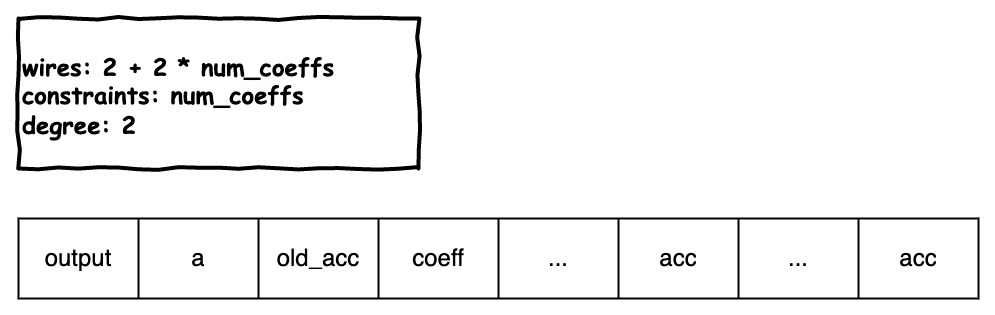
\includegraphics[width=0.5\textwidth]{gates/reducing.jpeg}
    \caption{ReducingGate}
    \label{fig:reducing}
\end{figure}

The constraint flow is relatively intuitive, initializing acc to old\_acc, then cumulative computation of polynomials by coeff in turn, 
and constraining the intermediate results of each step with acc.

\begin{lstlisting}[language=rust]
for i in 0..self.num_coeffs {
    let coeff = builder.convert_to_ext_algebra(coeffs[i]);
    let mut tmp = builder.mul_add_ext_algebra(acc, alpha, coeff);
    tmp = builder.sub_ext_algebra(tmp, accs[i]);
    constraints.push(tmp);
    acc = accs[i];
}
\end{lstlisting}

The number of constraints is equal to the number of coefficients. Polynomial degree is 2 which happens when calculating $\text{coeff}_i * \alpha$, sum up does not increase degree.

ReducingExtensionGate is like ReducingGate, just computations happen in extension field, constrain logic is all the same.

\paragraph{high\_degree\_interpolation}

InterpolationGate is used for interpolation a polynomial, whose points are a (base field) coset of the multiplicative subgroup 
with the given size, and whose values are extension field elements. As for HighDegreeInterpolationGate,  allows constraints of variable degree, 
up to \verb|1 << subgroup_bits|. The higher degree is a tradeoff for less gates (than LowDegreeInterpolationGate).


HighDegreeInterpolationGate trace is shown in \figref{fig:high-degree-interpolation}.

\begin{figure}[!ht]
    \centering
    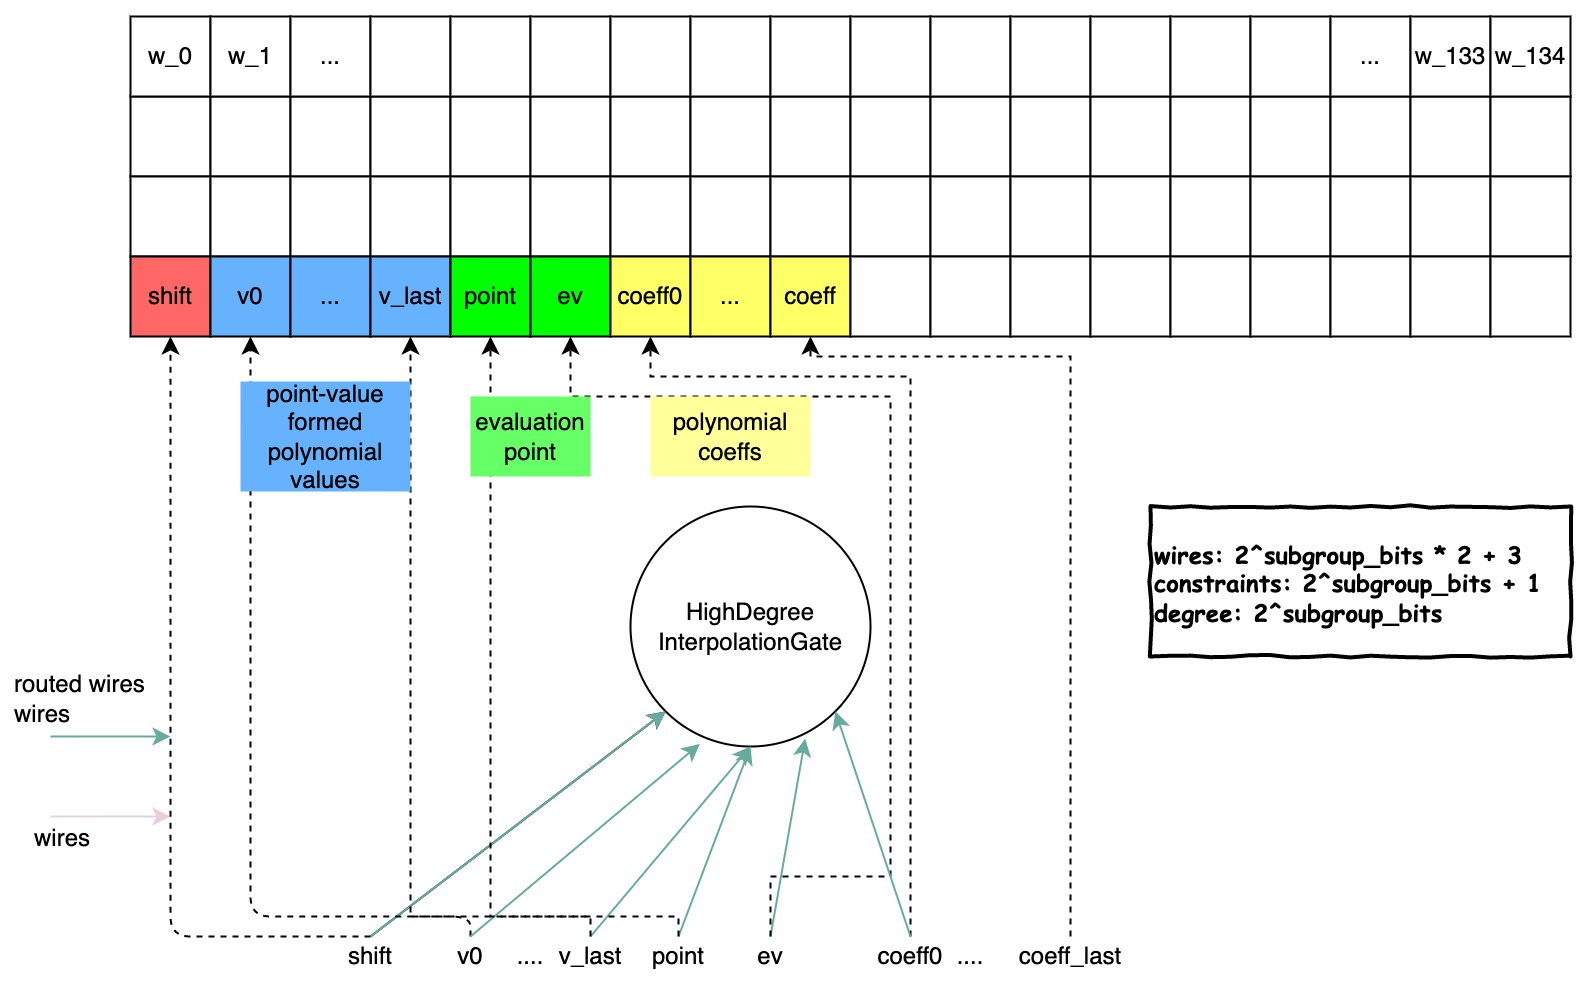
\includegraphics[width=0.6\textwidth]{gates/high_degree_interpolation.jpeg}
    \caption{HighDegreeInterpolationGate}
    \label{fig:high-degree-interpolation}
\end{figure}


Constraints:
\begin{itemize}
    \item Bring each point(from the point-value pairs) into the coefficient polynomial to compute the computed\_value, 
    and compare the constraint with the value(from the point-value pairs). -- A total of $2^{\text{subgroup\_bits}}$ constraints.
    \begin{lstlisting}
for (i, point) in coset.into_iter().enumerate() {
    let value = vars.get_local_ext_algebra(self.wires_value(i));
    let computed_value = interpolant.eval_base(point);
    constraints.extend((value - computed_value).to_basefield_array());
}
    \end{lstlisting}
    coset: $[sg, sg^2,...,sg^{2^{\text{subgroup\_bits}}}], \ s=\text{shift}$
    \item Evaluate the coefficient-form polynomial at evaluation point, and constrain with ev. -- 1 constraint.
\end{itemize}

The degree of this gate equals the number of points (num\_points): max point power is $\text{num\_points} - 1$, and multiplication by coefficient adds 1 degree.

Number of constraints equals $\text{num\_points} + 1$: num\_points for consistency between the coefficients and the point-value pairs, 1 constraints for the evaluation value. 

\paragraph{low\_degree\_interpolation}

InterpolationGate is used for the interpolation of a polynomial, whose points are a (base field) coset of the multiplicative subgroup 
with the given size, and whose values are extension field elements. As for LowDegreeInterpolationGate,  all constraints are degree <= 2, 
low degree is a tradeoff for more gates(than HighDegreeInterpolationGate).

LowDegreeInterpolationGate trace is shown in \figref{fig:low-degree-interpolation}.

\begin{figure}[!ht]
    \centering
    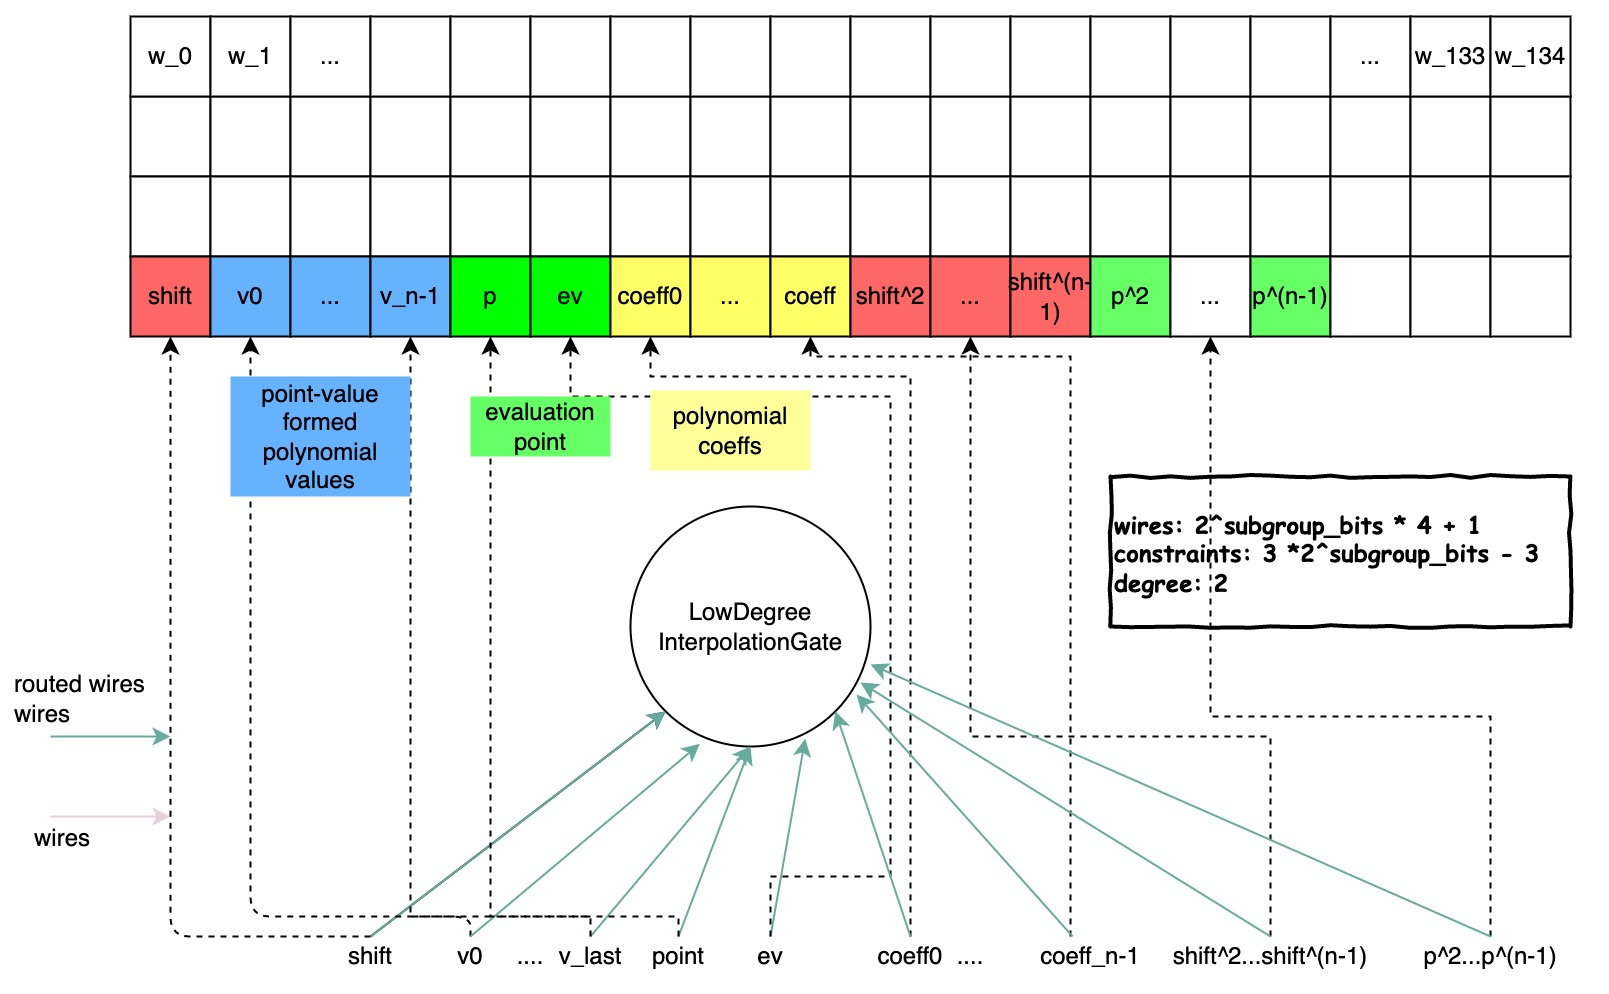
\includegraphics[width=0.6\textwidth]{gates/low_degree_interpolation.jpeg}
    \caption{LowDegreeInterpolationGate}
    \label{fig:low-degree-interpolation}
\end{figure}

Constraints:
\begin{itemize}
    \item Constrain powers of shift, from $\text{shift}^2$ to $\text{shift}^{n-1}$, a total of $2^{\text{subgroup\_bits}}-2$ constraints.
    \begin{lstlisting}[language=rust]
for i in 1..self.num_points() - 1 {
    constraints.push(powers_shift[i - 1] * shift - powers_shift[i]);
}
    \end{lstlisting}
    \item Bring each point (from the point-value pairs) into the coefficient polynomial to compute the computed\_value 
    and compare the constraint with the value (from the point-value pairs). -- A total of $2^{\text{subgroup\_bits}}$ constraints.
    \item Constrain powers of evaluation point. -- A total of $2^{\text{subgroup\_bits}}-2$ constraints.
    \item Evaluate the coefficient-form polynomial at the evaluation point and constrain it. -- 1 constraint.
\end{itemize}

As can be seen from the above constraint description, the number of constraints is $3*2^{\text{subgroup\_bits}}-3$, degree of LowDegreeInterpolationGate is 2.

\subsubsubsection{U32 gates}
\subsubsubsection{add\_many\_u32}

\hspace*{\fill}

\indent U32AddManyGate is a gate to perform addition on num\_addends different 32-bit values, plus a small carry. 
There can be up to 16 operations per gate.

The gate structure is like \figref{fig:add-many-u32}.

\begin{figure}[!ht]
    \centering
    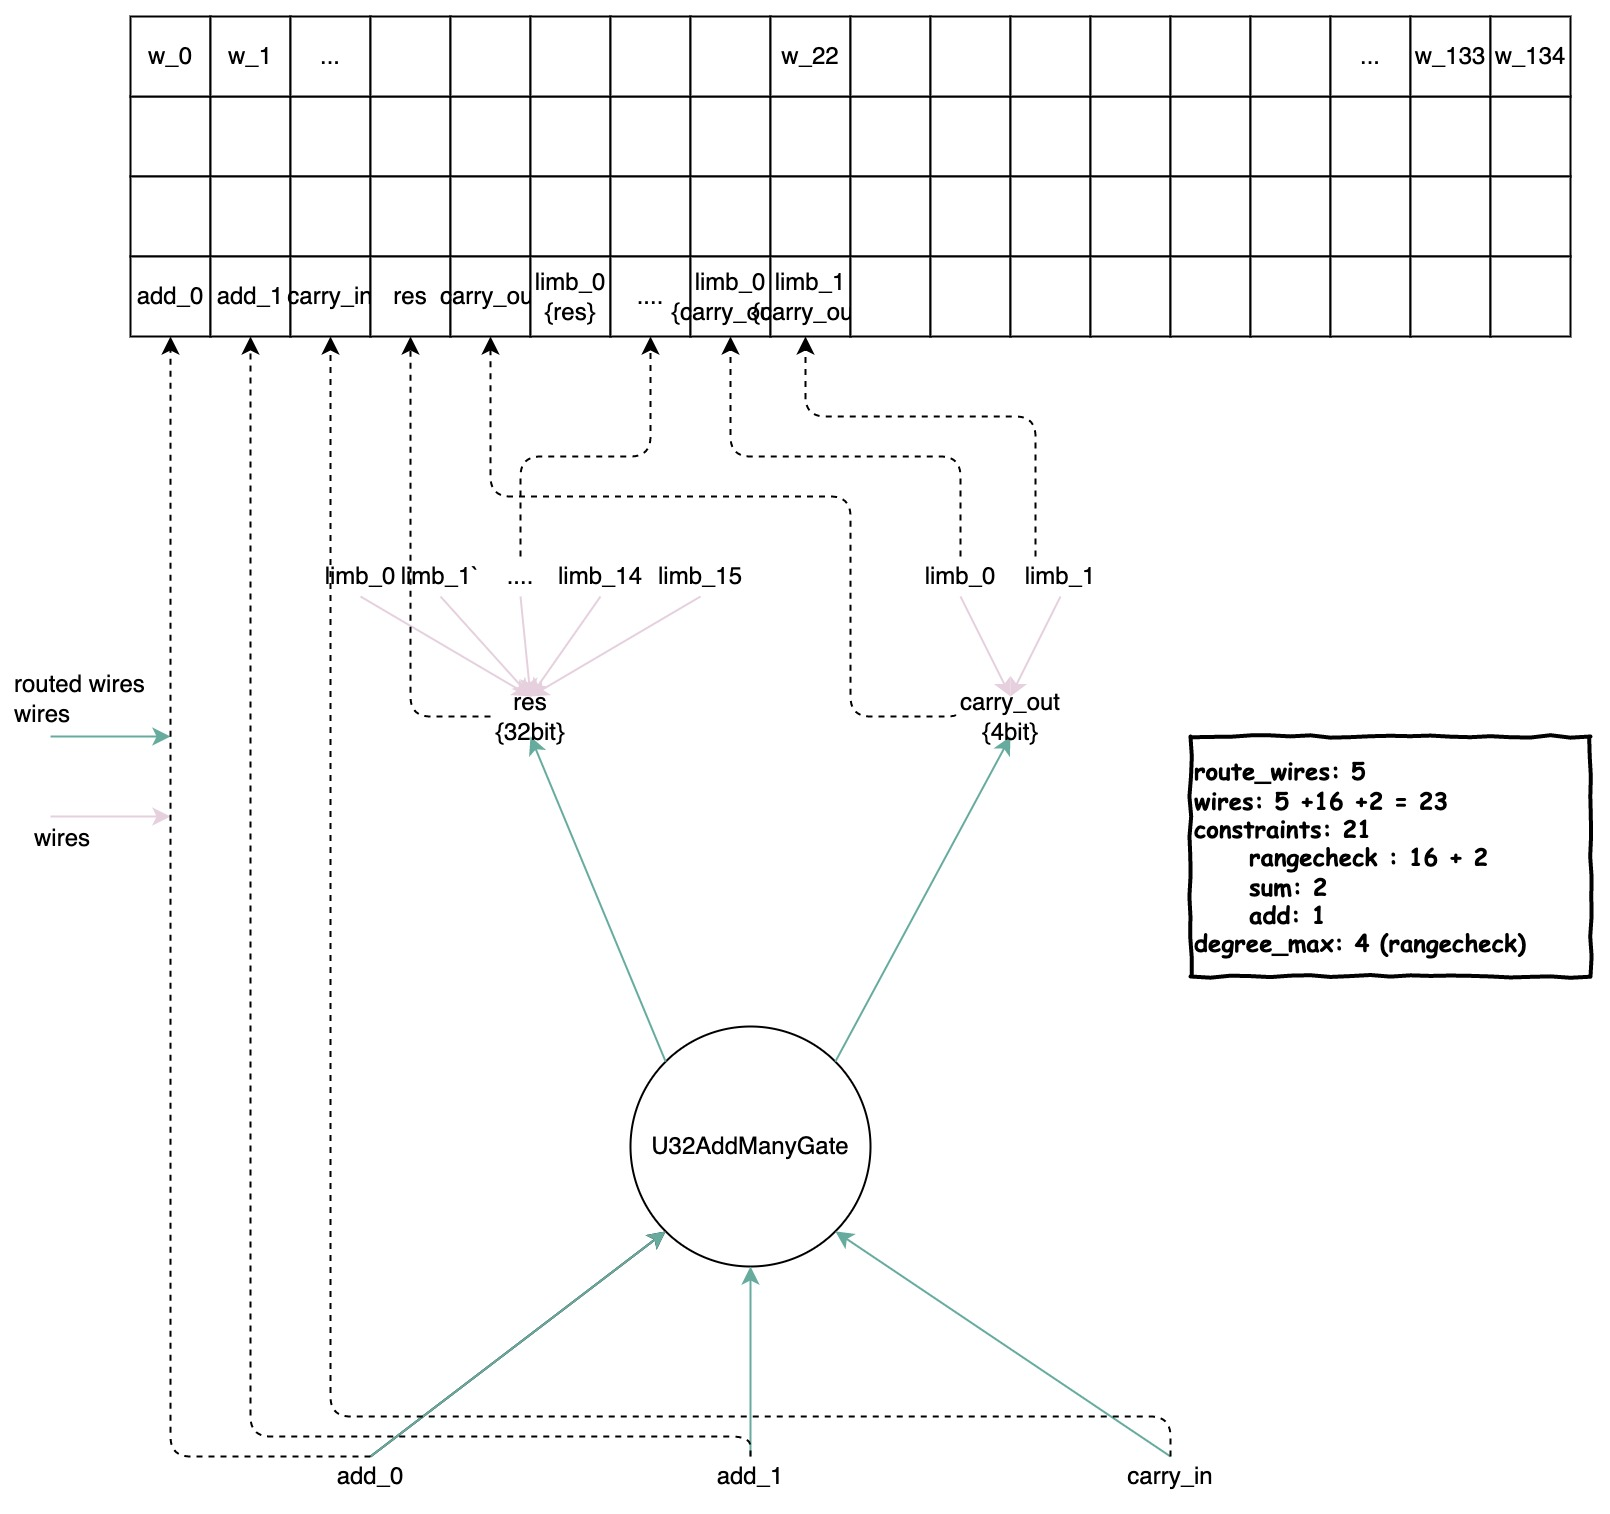
\includegraphics[width=0.6\textwidth]{gates/add_many_u32.jpeg}
    \caption{U32AddManyGate}
    \label{fig:add-many-u32}
\end{figure}

Constraints for each operation:
\begin{itemize}
    \item Constrain the result of addends summation equals results of res and carry\_out calculation. -- 1 constraint with degree 1
    \begin{lstlisting}[language=rust]
let base = F::Extension::from_canonical_u64(1 << 32u64);
let combined_output = output_carry * base + output_result;
constraints.push(combined_output - computed_output);
    \end{lstlisting}
    \item Limbs range check. -- 18(limbs) constraints with degree 4.(limbs are all 2-bits)
    \begin{lstlisting}[language=rust]
let product = (0..max_limb)
    .map(|x| this_limb - F::Extension::from_canonical_usize(x))
    .product();
constraints.push(product);
    \end{lstlisting}
    \item Constrain limbs for res and carry\_out. -- 2 constraints with degree 1.
\end{itemize}

In summary, there are 21 constraints for each operation. The degree of the gate is 4 which is needed by the 4-bits limbs range check.

\paragraph{arithmetic\_u32}

U32ArithmeticGate gate is used for compute $\text{res} = \text{mul\_0} \times \text{mul\_1} + \text{add}$. Res is store in res\_lo and res\_hi each of which can be represented by 15 limbs.

Gate structure is like \figref{fig:arithmetic-u32}.

\begin{figure}[!ht]
    \centering
    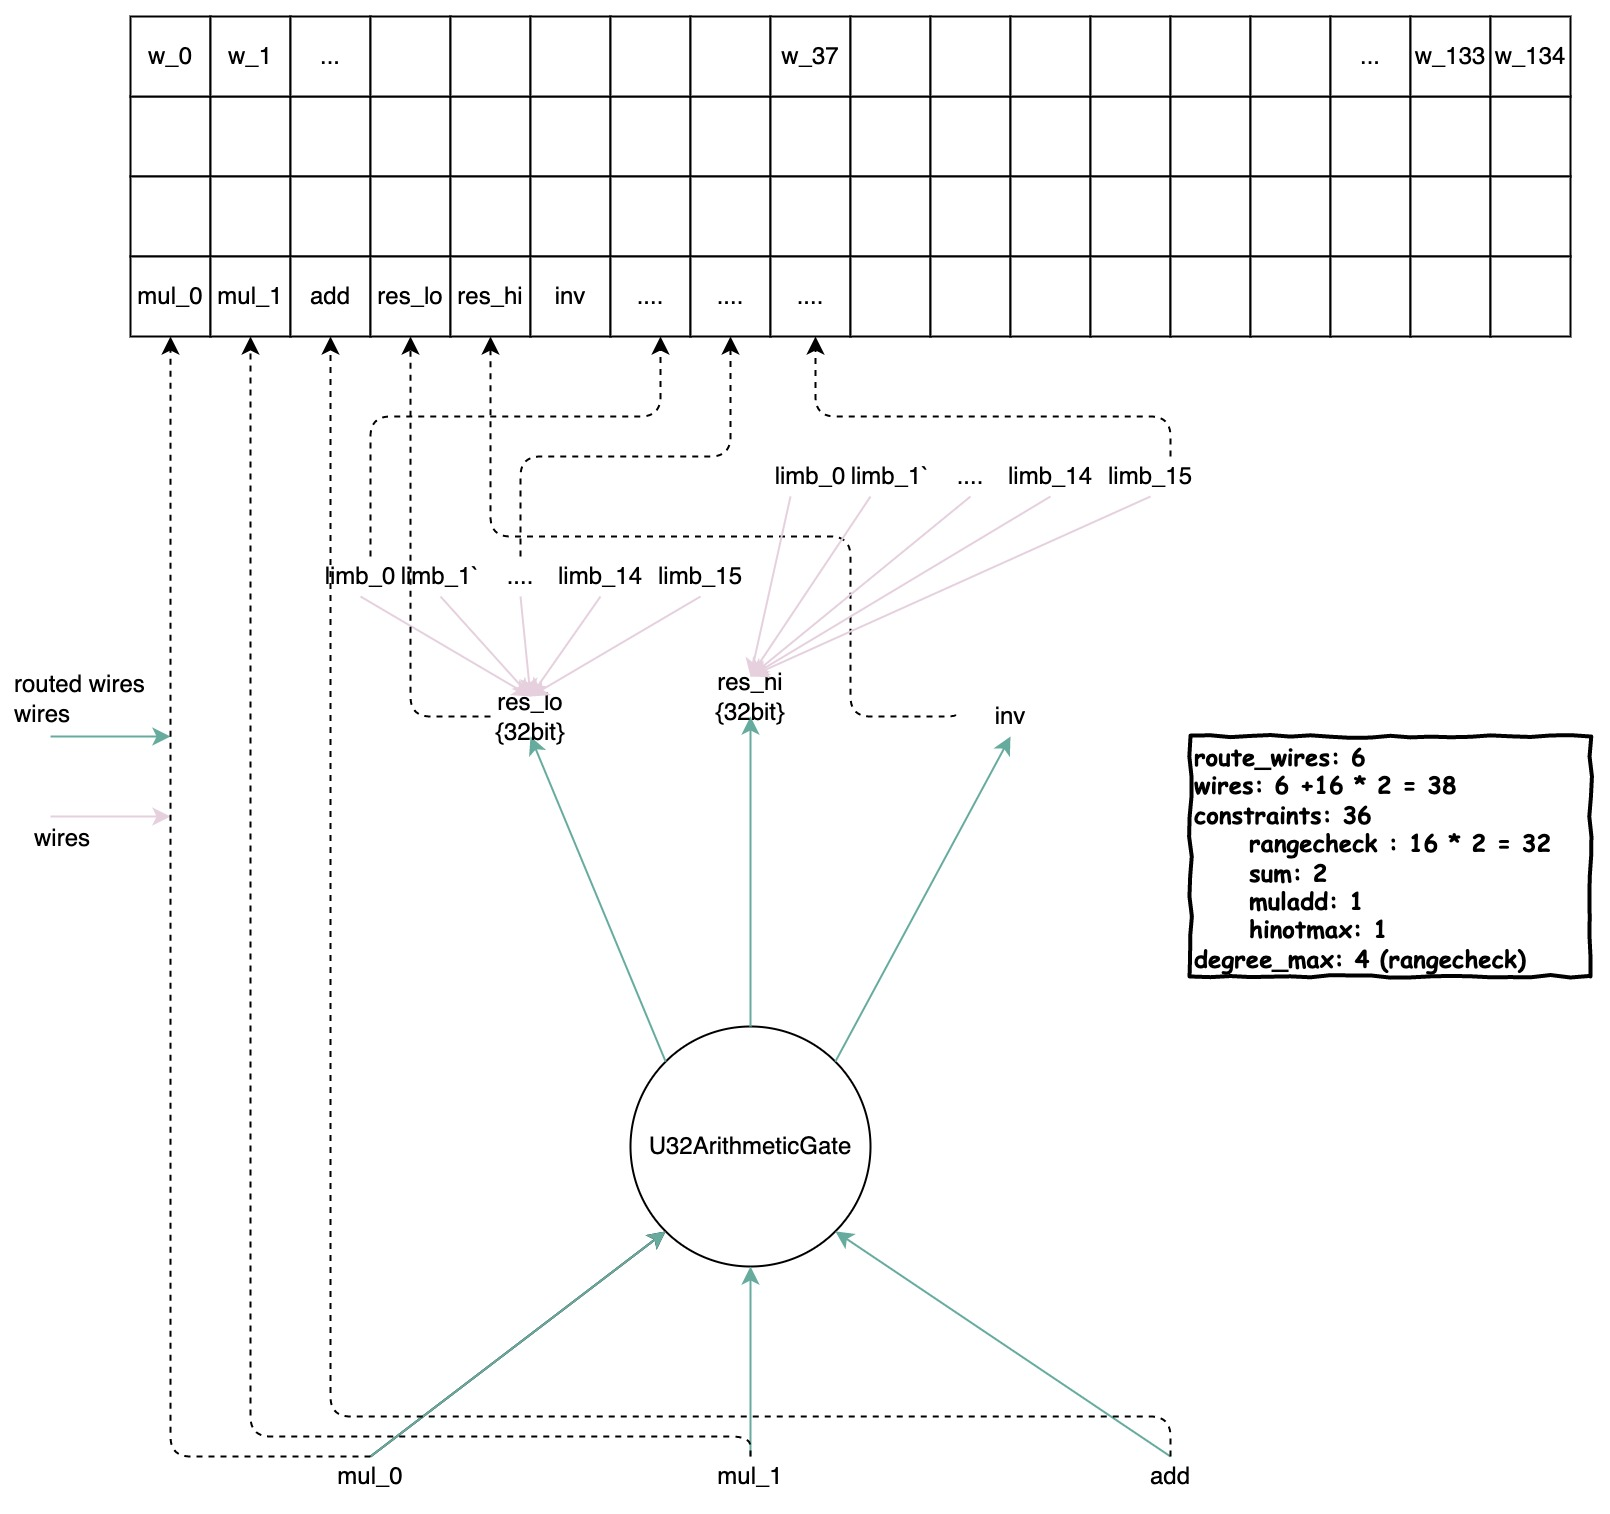
\includegraphics[width=0.8\textwidth]{gates/arithmetic_u32.jpeg}
    \caption{U32ArithmeticGate}
    \label{fig:arithmetic-u32}
\end{figure}

Constraints for each operation:
\begin{itemize}
    \item Constrain res is not overflow (less equal than \verb|max_u32 * max_u32 + max_u32|). -- 1 constraint with degree 2.
    \item Constrain combined((by res\_lo and res\_hi)) output equals computed (by \verb|mul_0 * mul_1 + add|) output. -- 1 constraint with degree 2.
    \item Limbs range check. -- 32 (limbs) constraints with degree 4. (limbs are all 2-bits)
    \item Constrain limbs for res\_lo and res\_hi. -- 2 constraints with degree 1.
\end{itemize}

In summary, there are 36 constraints for each operation. Degree of the gate is 4 which is needed by 4-bits limbs range check.

\subsubsubsection{comparison}

\hspace*{\fill}

\indent ComparisonGate is a gate for checking that one value is less than or equal to another. 
Compared numbers are divided into chunks, and chunk size and the number are configurable.

For a ComparisonGate with 8 4-bits chunks is like \figref{fig:comparison}.

\begin{figure}[!ht]
    \centering
    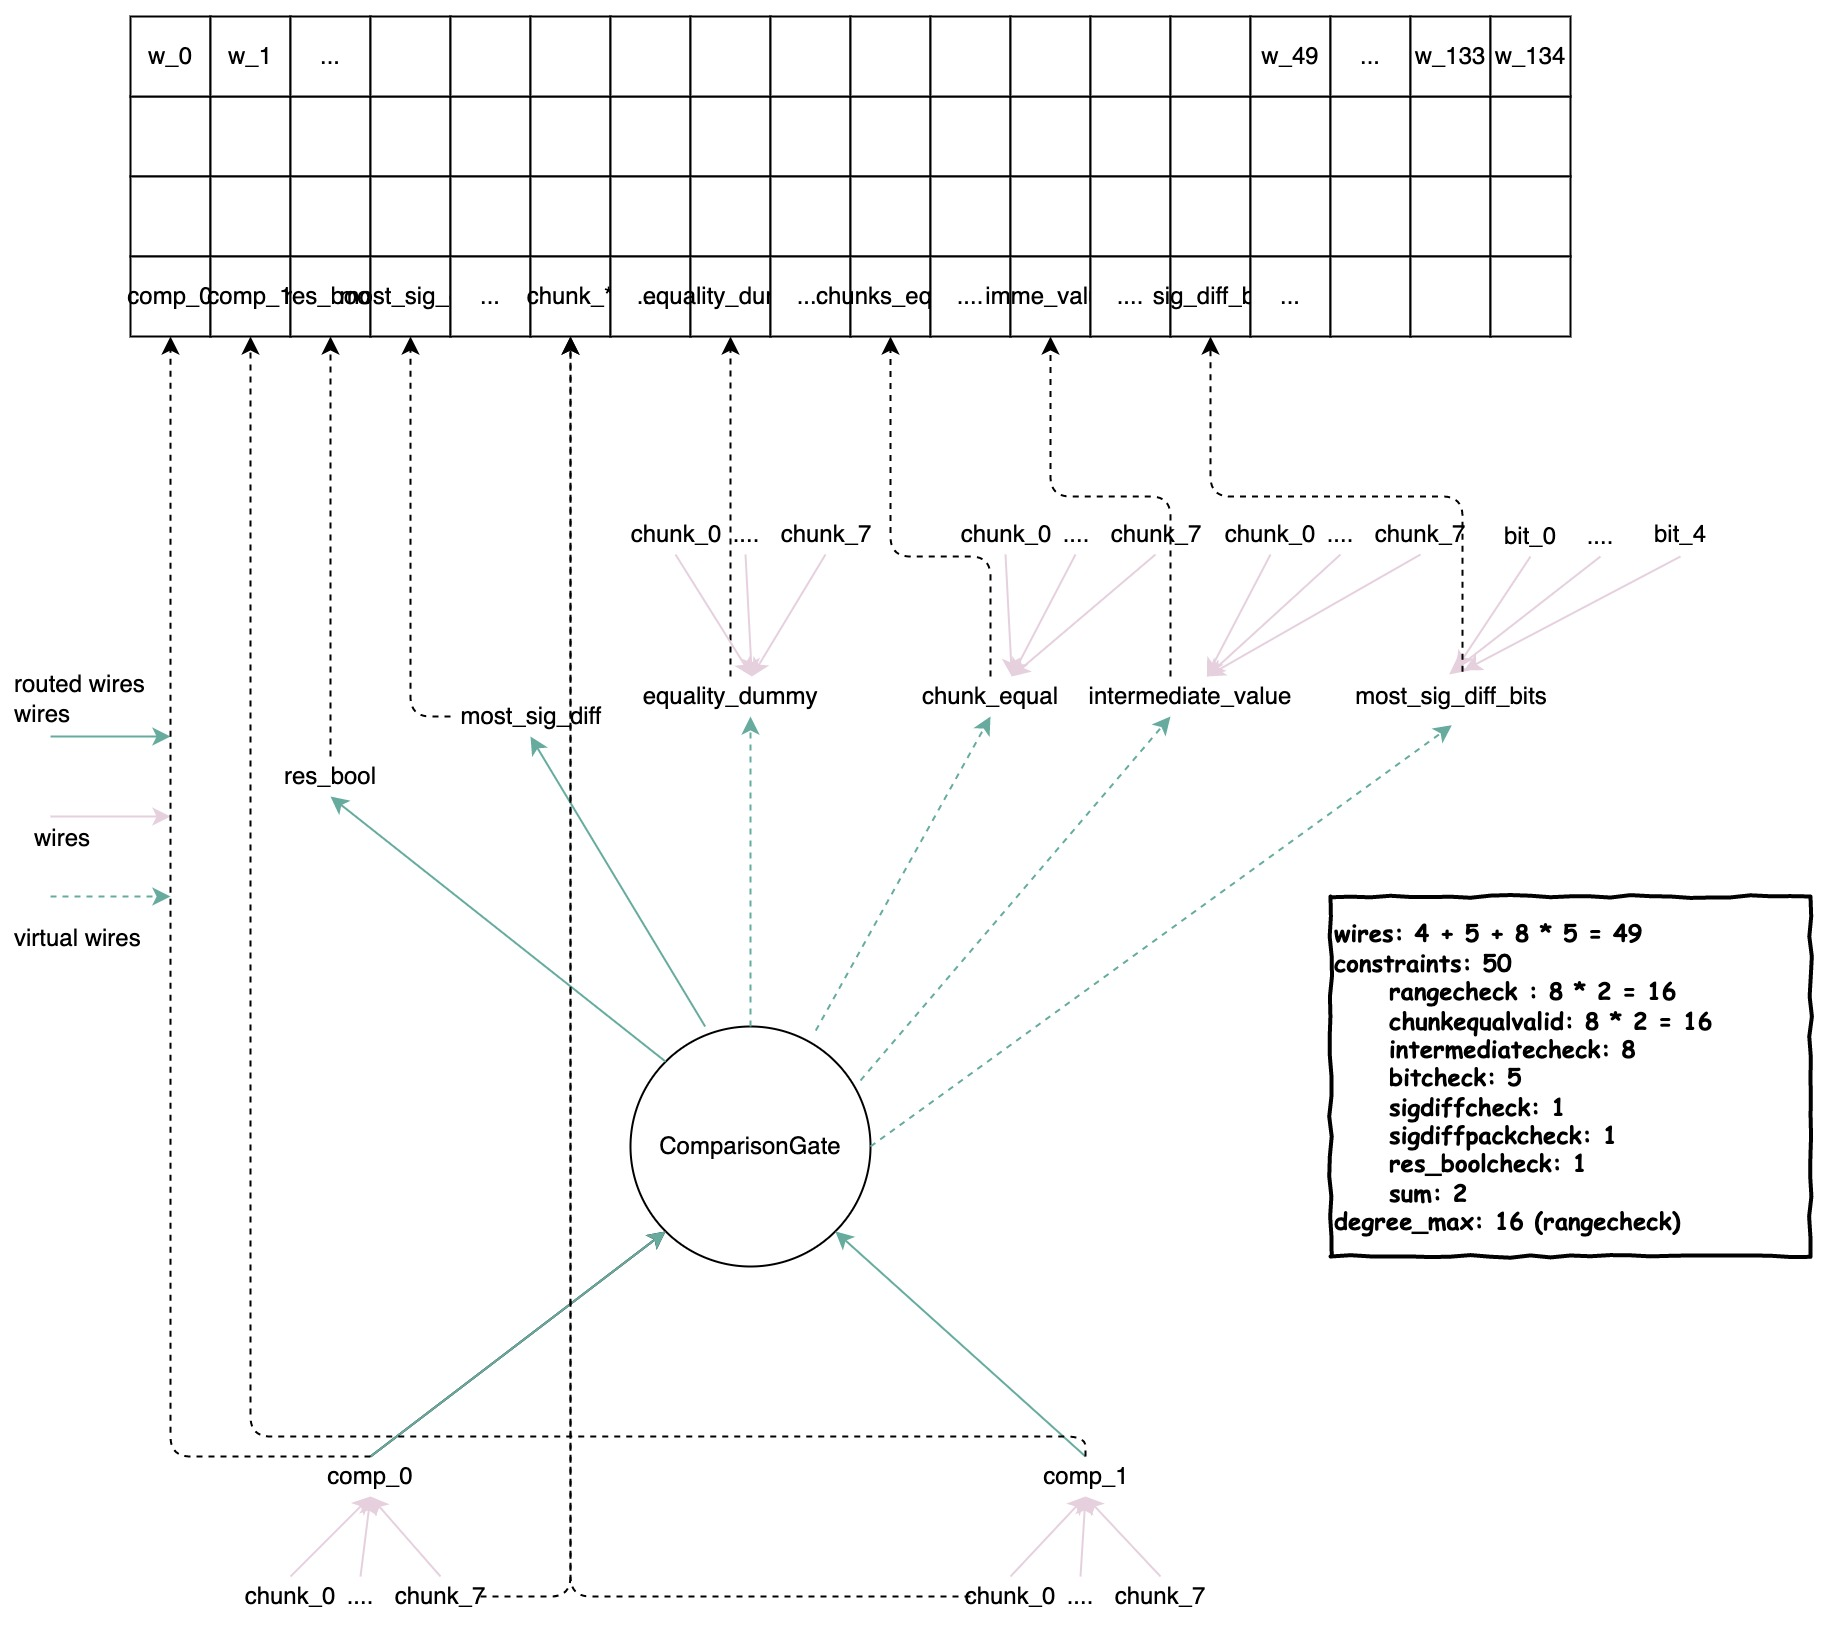
\includegraphics[width=0.6\textwidth]{gates/comparison.jpeg}
    \caption{ComparisonGate}
    \label{fig:comparison}
\end{figure}

The main idea of constraints:
\begin{itemize}
    \item Consistency of the sliced chunks and the original values.
    \item Range check for each chunk.
    \item If the chunks are equal, the difference is 0 and there is no inverse.
    \item Chunk by chunk so for most significant diff equals related intermediate\_value.
    \item If first <= second, the top \verb|n+1|-th bit of $(2^n + \text{most\_significant\_diff})$ will be 1.
\end{itemize}

\paragraph{range\_check\_u32}

U32RangeCheckGate is a gate that can decompose a number into base B little-endian limbs.

The gate structure is like \figref{fig:range-check-u32}.

\begin{figure}[!ht]
    \centering
    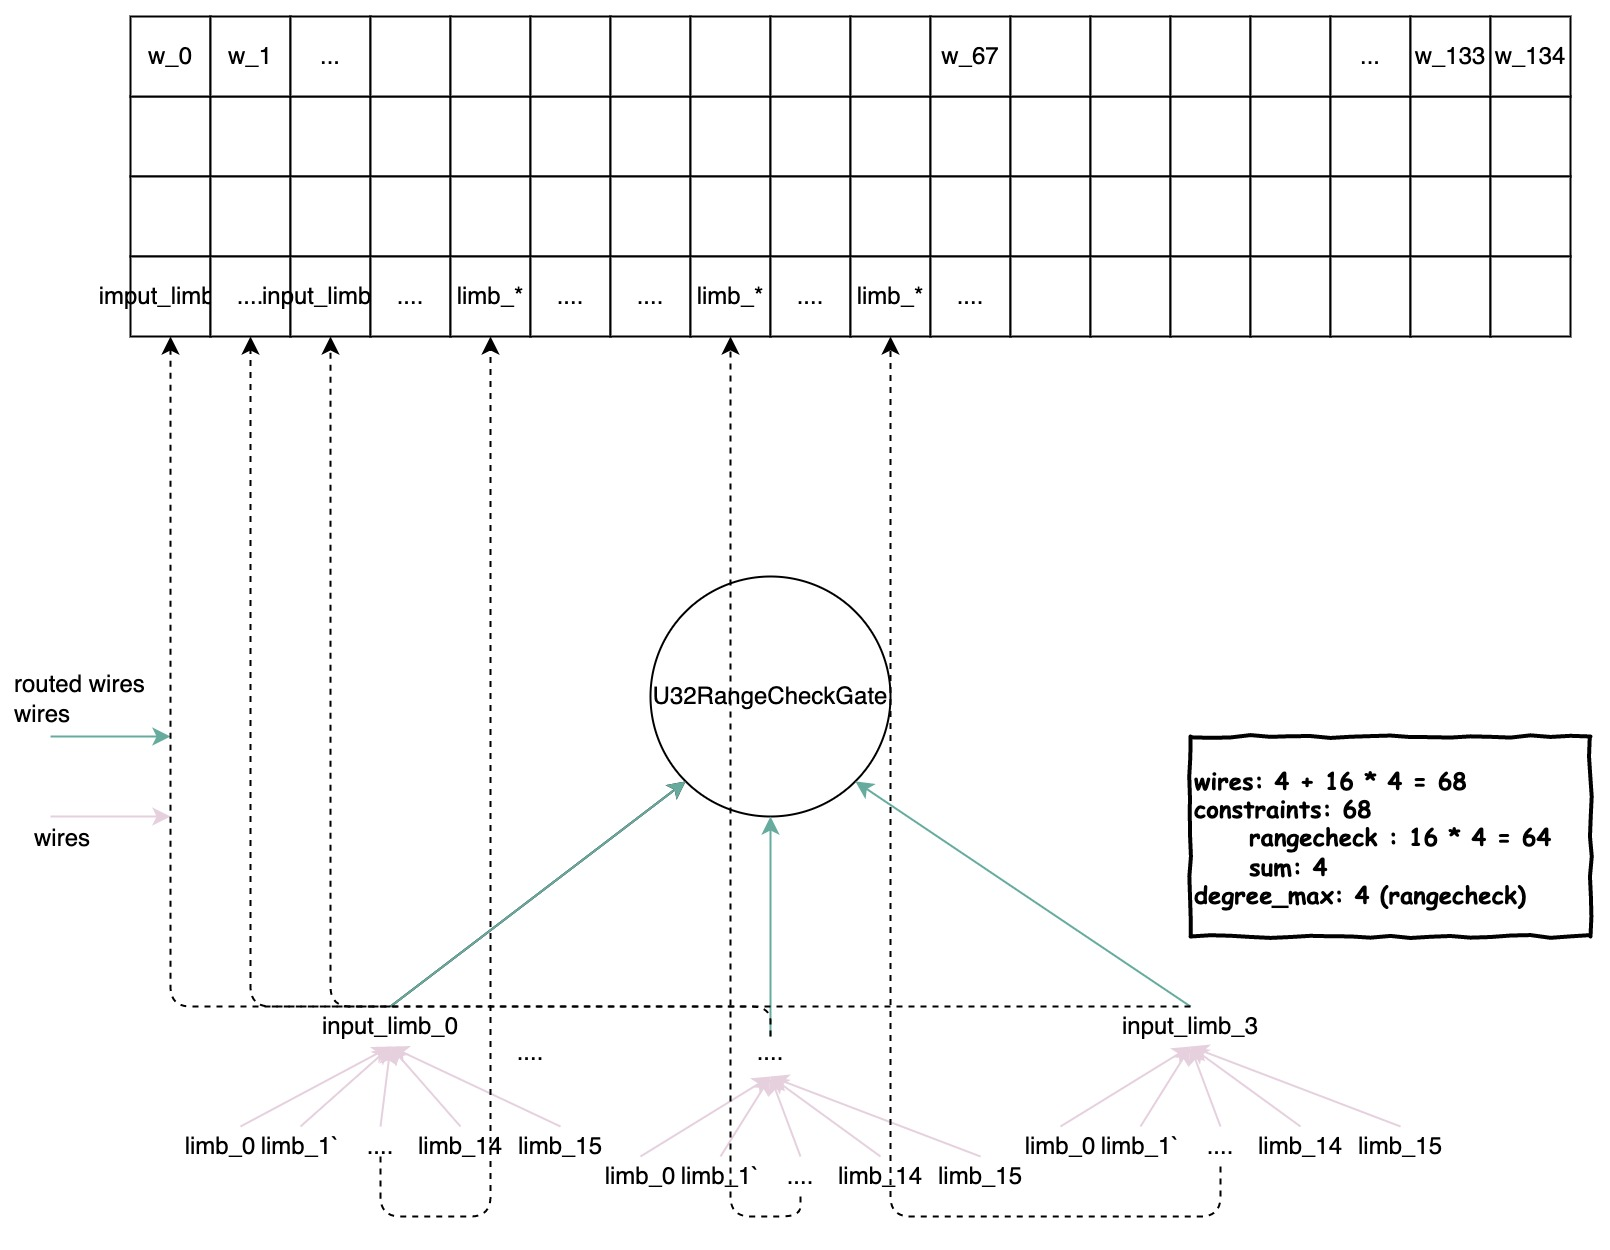
\includegraphics[width=0.6\textwidth]{gates/range_check_u32.jpeg}
    \caption{U32RangeCheckGate}
    \label{fig:range-check-u32}
\end{figure}

Constraints for each input\_limb:
\begin{itemize}
    \item Each input\_limb consists of its aux\_limbs. -- 1 constraint with degree 1.
    \begin{lstlisting}[language=rust]
let computed_sum = reduce_with_powers(&aux_limbs, base);
constraints.push(computed_sum - input_limb);
    \end{lstlisting}
    \item aux\_limbs range check. -- 16 (aux\_limbs) constraints with degree BASE ($(x-0)(x-1)\cdots(x-\text{BASE}+1)$).
\end{itemize}

In summary, there are 17 constraints per input limb, a total of $\text{num\_input\_limbs} \times 17$ constraints. 
The degree of the gate equals BASE for range check.

\subsubsubsection{subtraction\_u32}

\hspace*{\fill}

\indent U32SubtractionGate is a gate to perform subtraction on 32-bit limbs: given `x', `y', and `borrow', it returns 
the result $x - y - \text{borrow}$ and, if this underflows, a new `borrow'.

The gate structure is like \figref{fig:subtraction-u32}.

\begin{figure}[!ht]
    \centering
    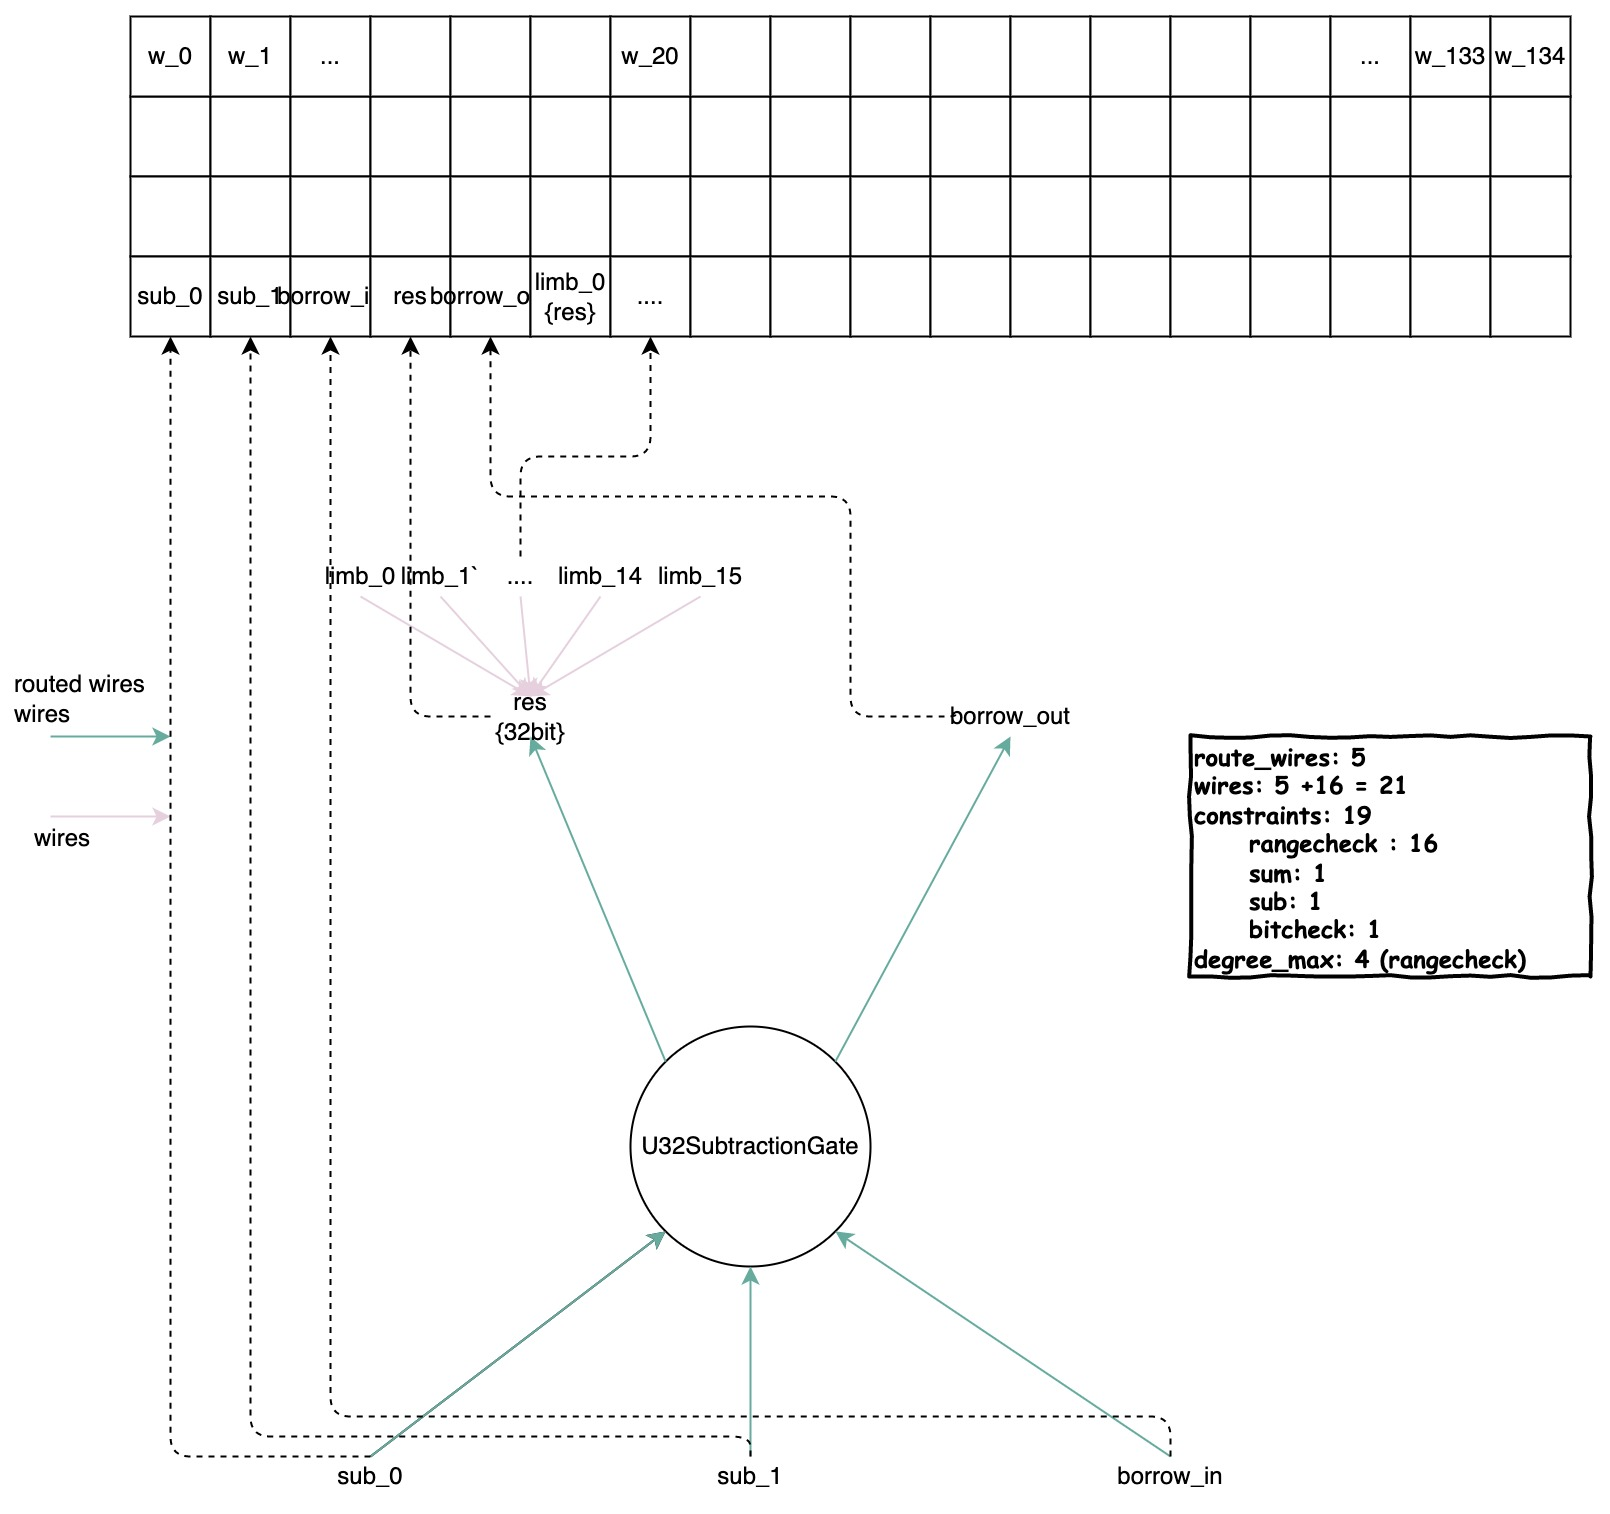
\includegraphics[width=0.6\textwidth]{gates/subtraction_u32.jpeg}
    \caption{U32SubtractionGate}
    \label{fig:subtraction-u32}
\end{figure}

Constraints for each operation:
\begin{itemize}
    \item Constrain the calculation. -- 1 constraint with degree 2.
    \begin{lstlisting}[language=rust]
let result_initial = input_x - input_y - input_borrow;
...
constraints.push(output_result - (result_initial + base * output_borrow));
    \end{lstlisting}
    \item Limbs range check. -- 16 (limbs) constraints with degree 4. (limbs are all 2-bits)
    \item Constrain limbs for res. -- 1 constraint with degree 1.
    \item Constrain borrow\_out to be one bit. -- 1 constraint with degree 1.
\end{itemize}

In summary, there are 19 constraints for each operation. The degree of the gate is 4 which is needed by the 4-bits limbs range check.

\subsubsection{Gadgets}



\subsubsubsection{biguint-add}

\begin{enumerate}
    \item \verb|Target|: Implement the addition of two biguints.
    \item \verb|Constraints logic|: 
        \begin{itemize}
            \item Equation for gates;
            \item Sumcheck between output and limbs;
            \item Rangecheck for limbs.
        \end{itemize}
    \item \verb|Circuit layout|: See \figref{fig:biguint-add-circuit-layout}.
    \item \verb|Trace layout|: See \figref{fig:biguint-add-trace-layout}.
    \item \verb|Constraints info and costs|
    \begin{itemize}
        \item gate type num: 1 (U32AddManyGate)
        \item gate ops num: limbs-num
        \item gate instance num: ceil(limbs-num / gate.ops)
        \item copy-constraints: limbs-num * 4
        \item max-degree: 4 (\verb|1 << limb-bits|)
    \end{itemize}
\end{enumerate}

\begin{figure}[!ht]
    \centering
    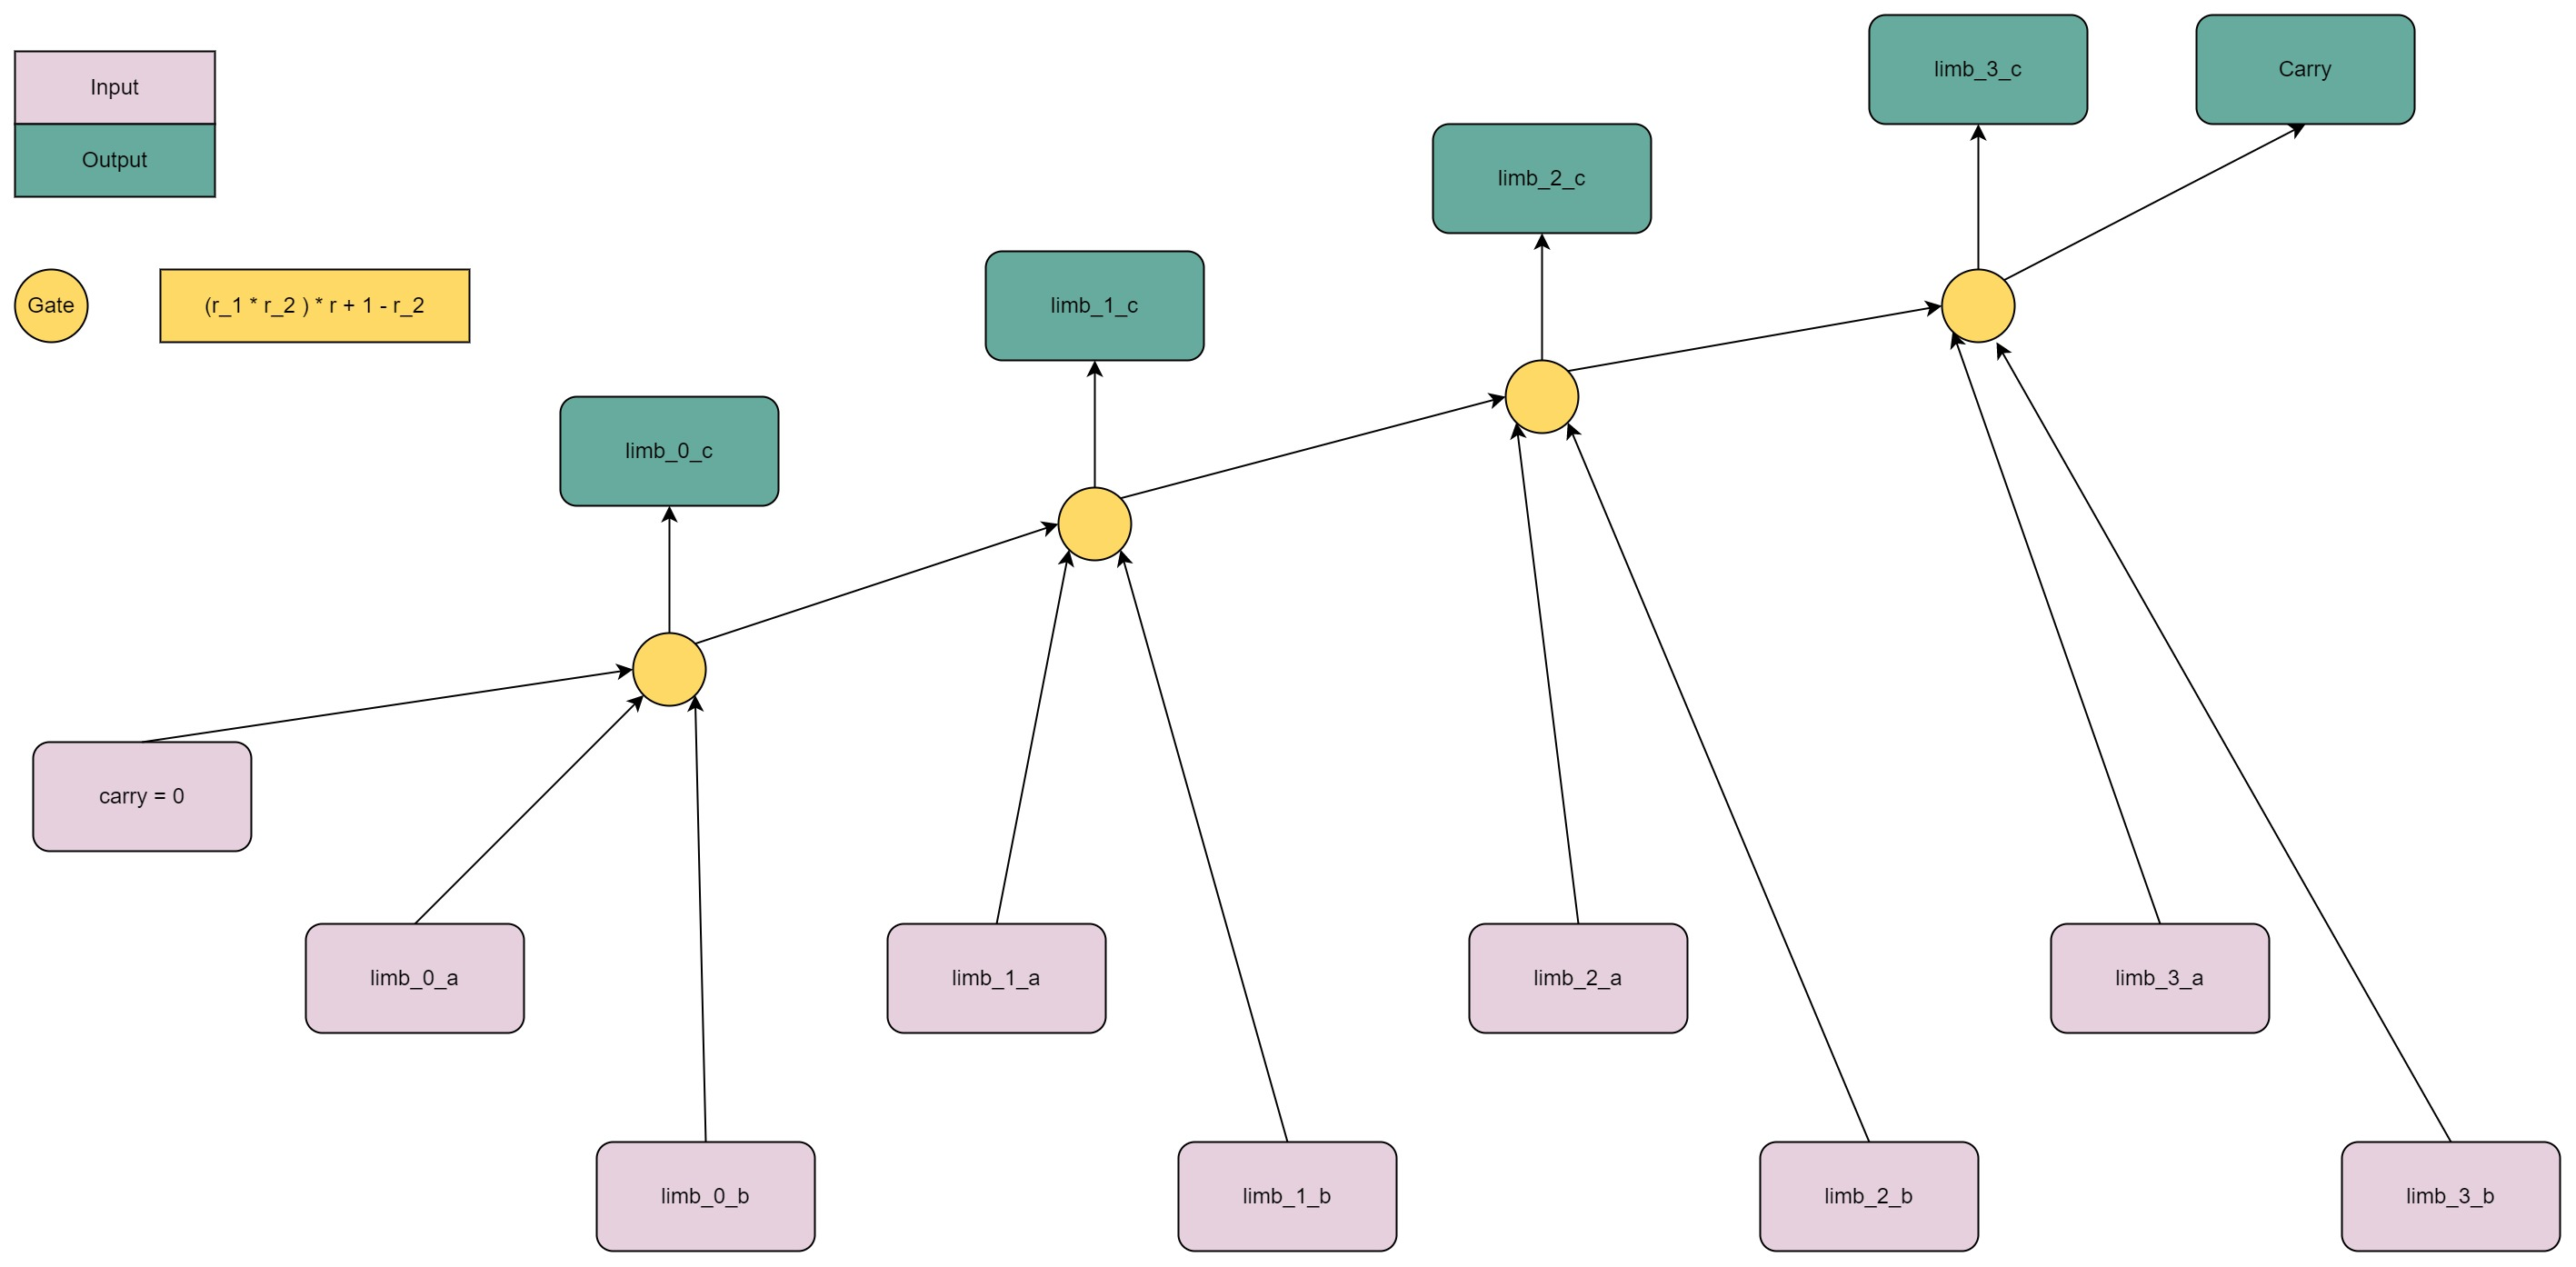
\includegraphics[width=0.6\textwidth]{biguint-add-circuit-layout.jpg}
    \caption{biguint-add circuit layout}
    \label{fig:biguint-add-circuit-layout}
\end{figure}
 
\begin{figure}[!ht]
    \centering
    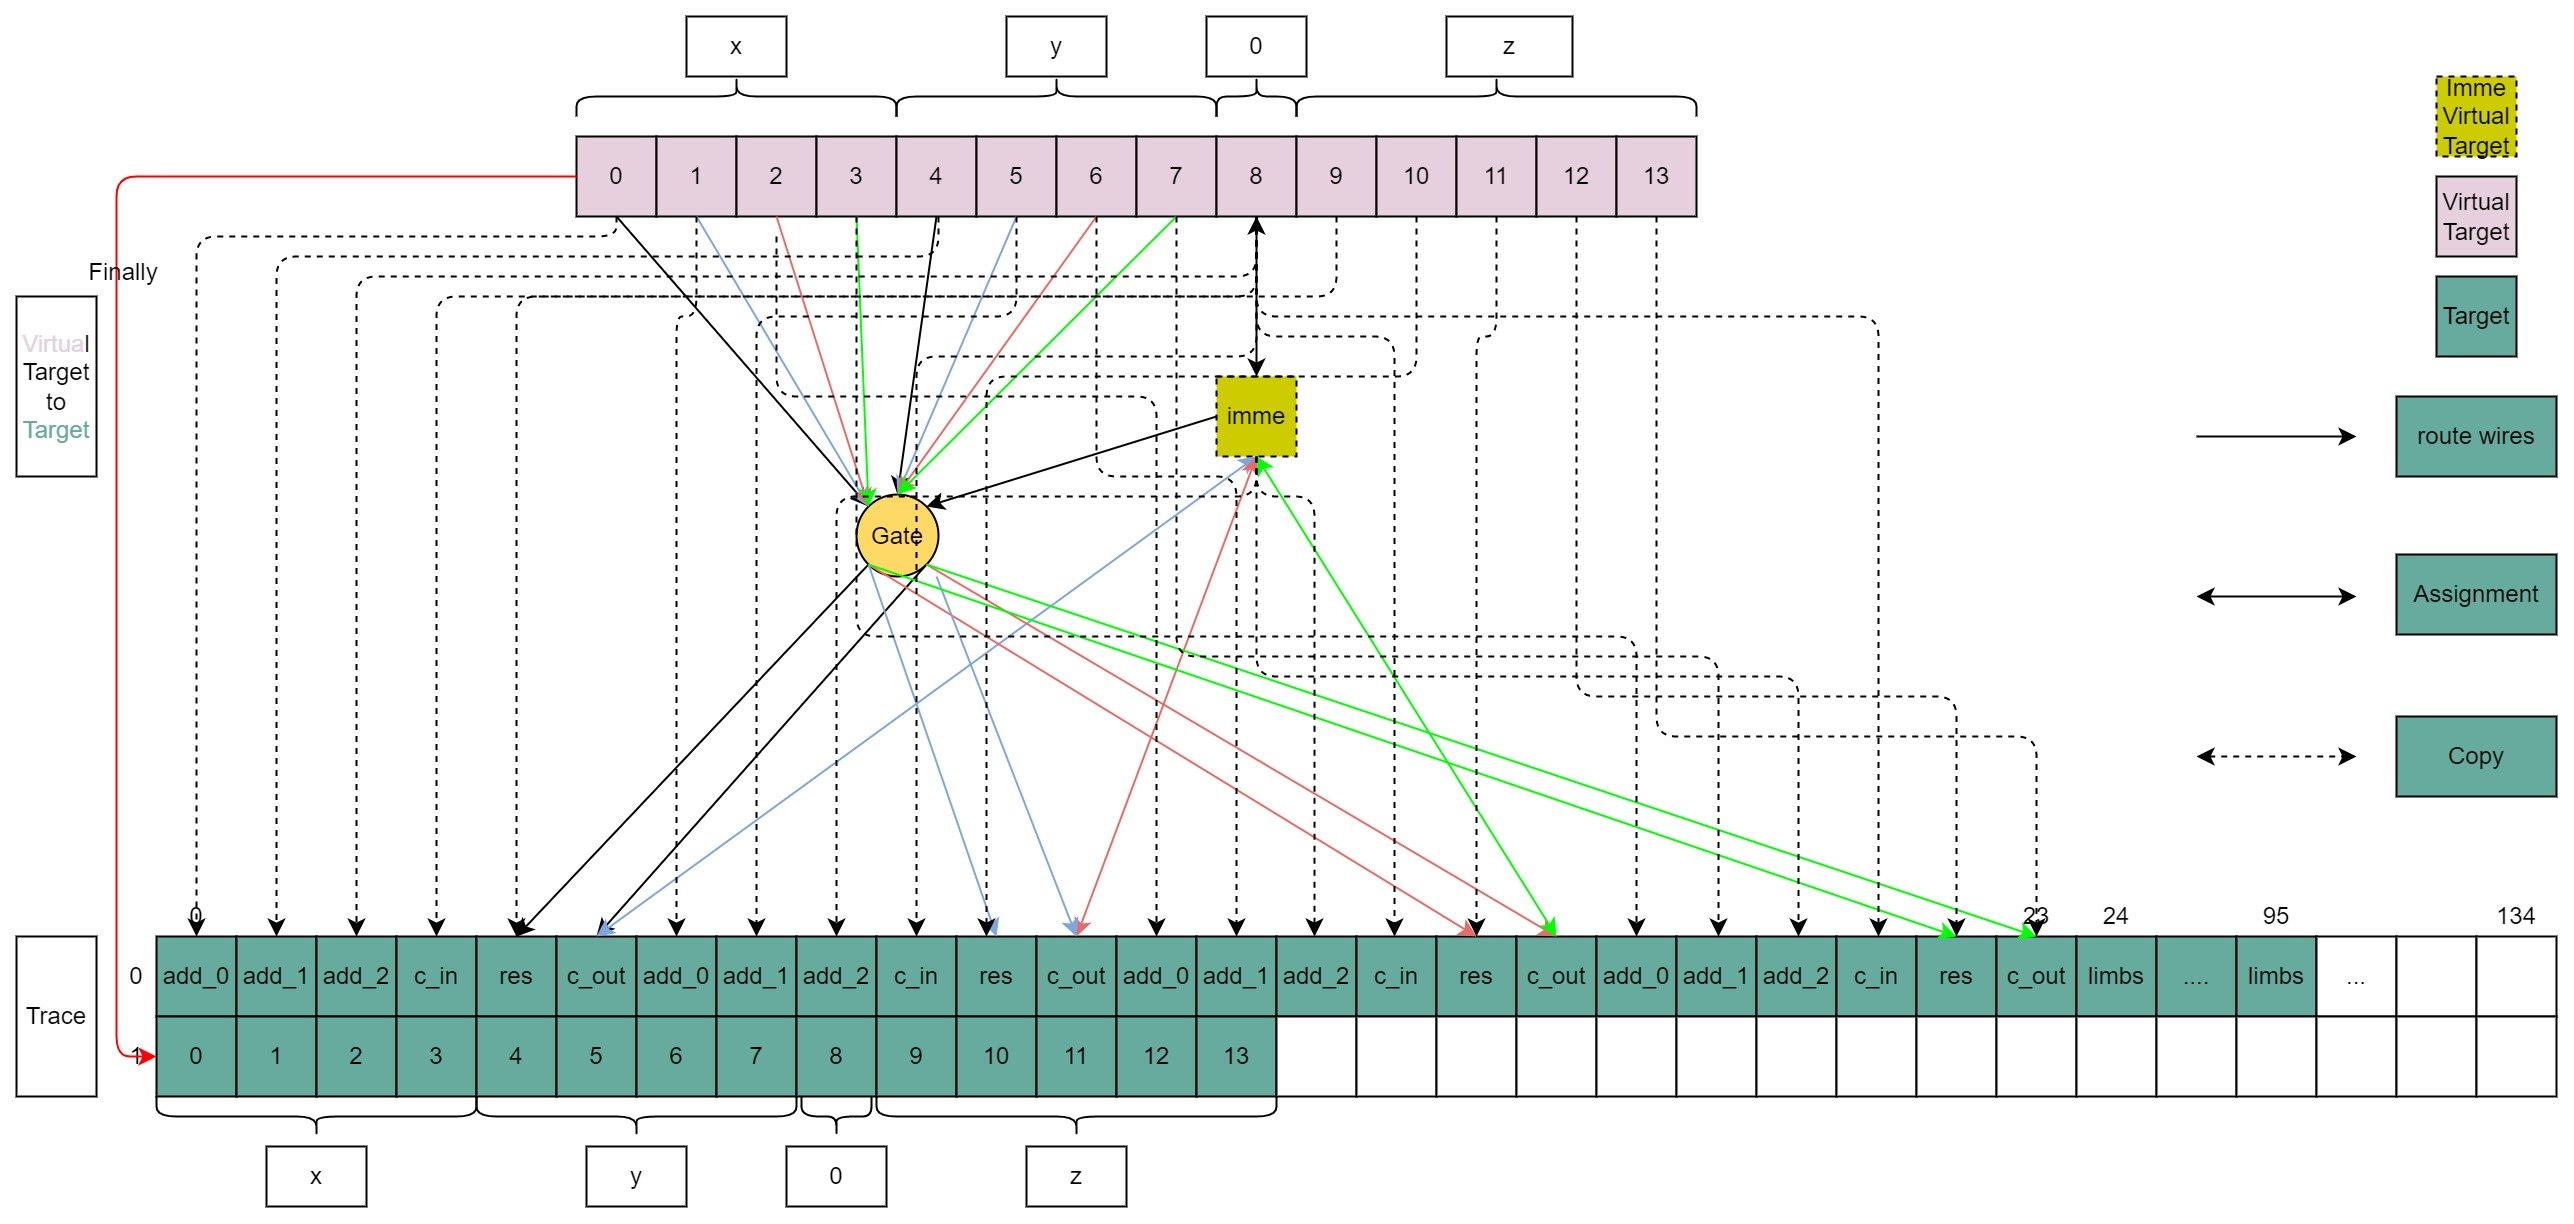
\includegraphics[width=0.6\textwidth]{biguint-add-trace-layout.jpg}
    \caption{biguint-add trace layout}
    \label{fig:biguint-add-trace-layout}
\end{figure}

\subsubsubsection{biguint-sub}

\begin{enumerate}
    \item \verb|Target|: Implement the substraction of two biguints.
    \item \verb|Constraints logic|:
    \begin{itemize}
        \item Equation for gate;
        \item Sumcheck for ouptput;
        \item Rangecheck for limbs.
    \end{itemize}
    \item \verb|Circuit layout|: See \ref{fig:biguint-sub-circuit-layout}.
    \item \verb|Trace layout|: See \ref{fig:biguint-sub-trace-layout}.
    \item \verb|Constraints info and costs|:
    \begin{itemize}
        \item constraints-num: $6 \times (3 + 32 / 2) = 114$
        \item copy-constraints: $16$
        \item max-degree: $4$
        \item wires-num: $6 \times (5 + 16) = 126$
    \end{itemize}
\end{enumerate}

\begin{figure}[!ht]
    \centering
    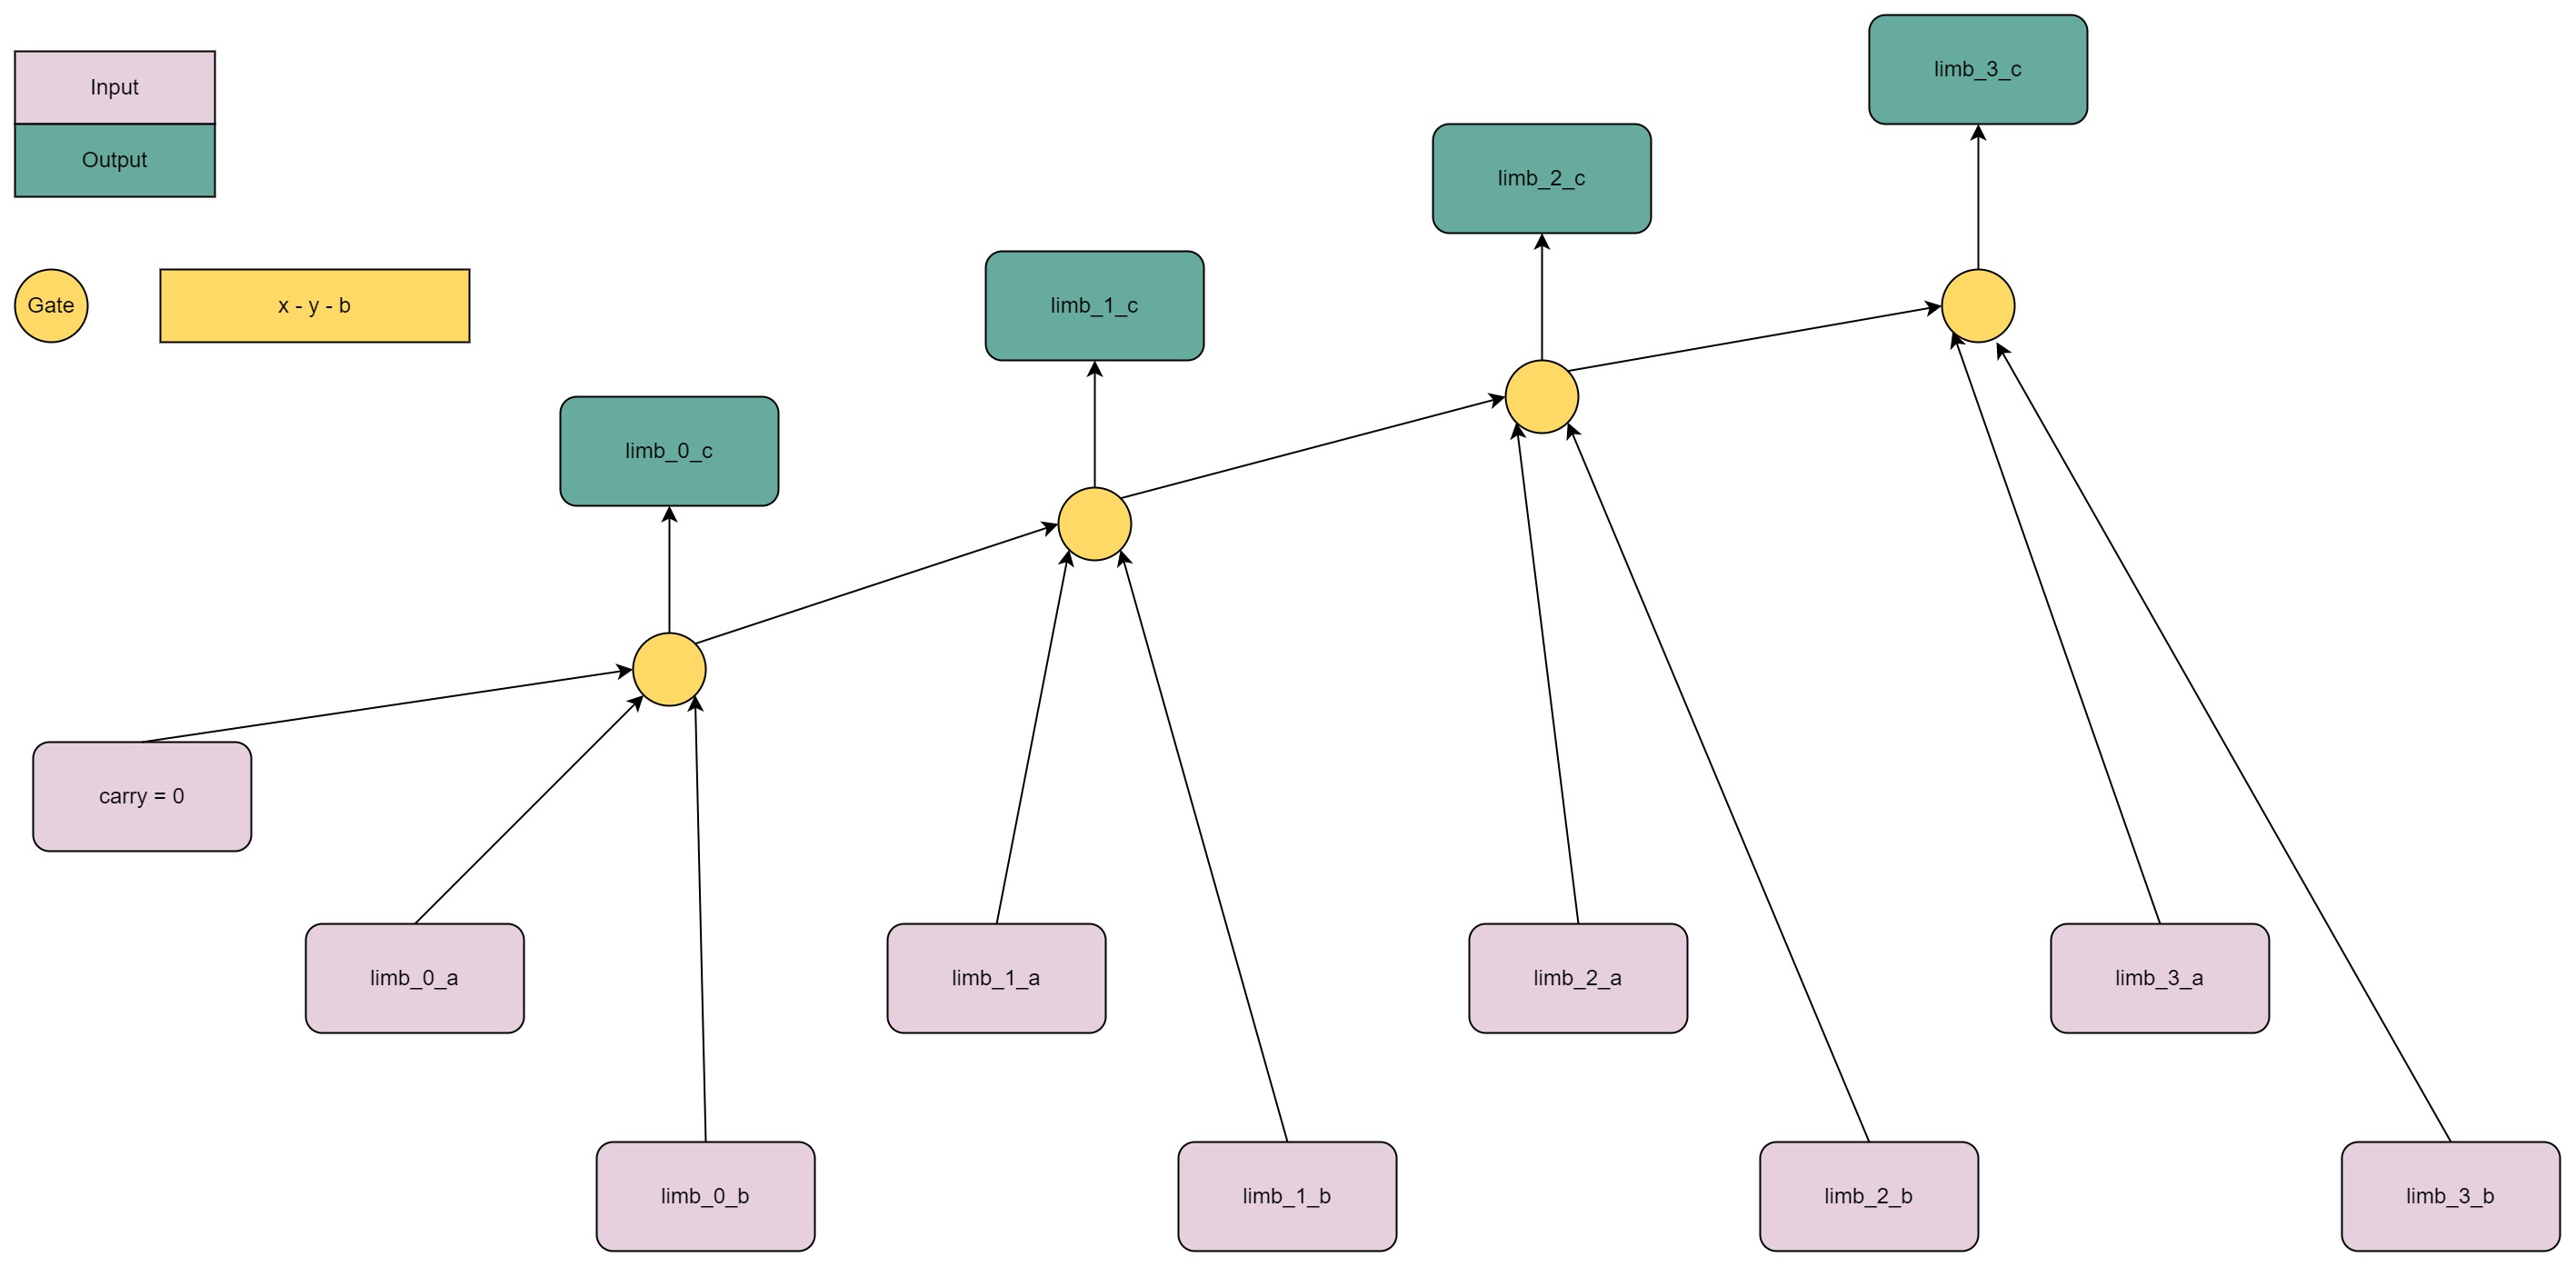
\includegraphics[width=0.6\textwidth]{biguint-sub-circuit-layout.jpg}
    \caption{biguint-sub circuit layout}
    \label{fig:biguint-sub-circuit-layout}
\end{figure}

\begin{figure}[!ht]
    \centering
    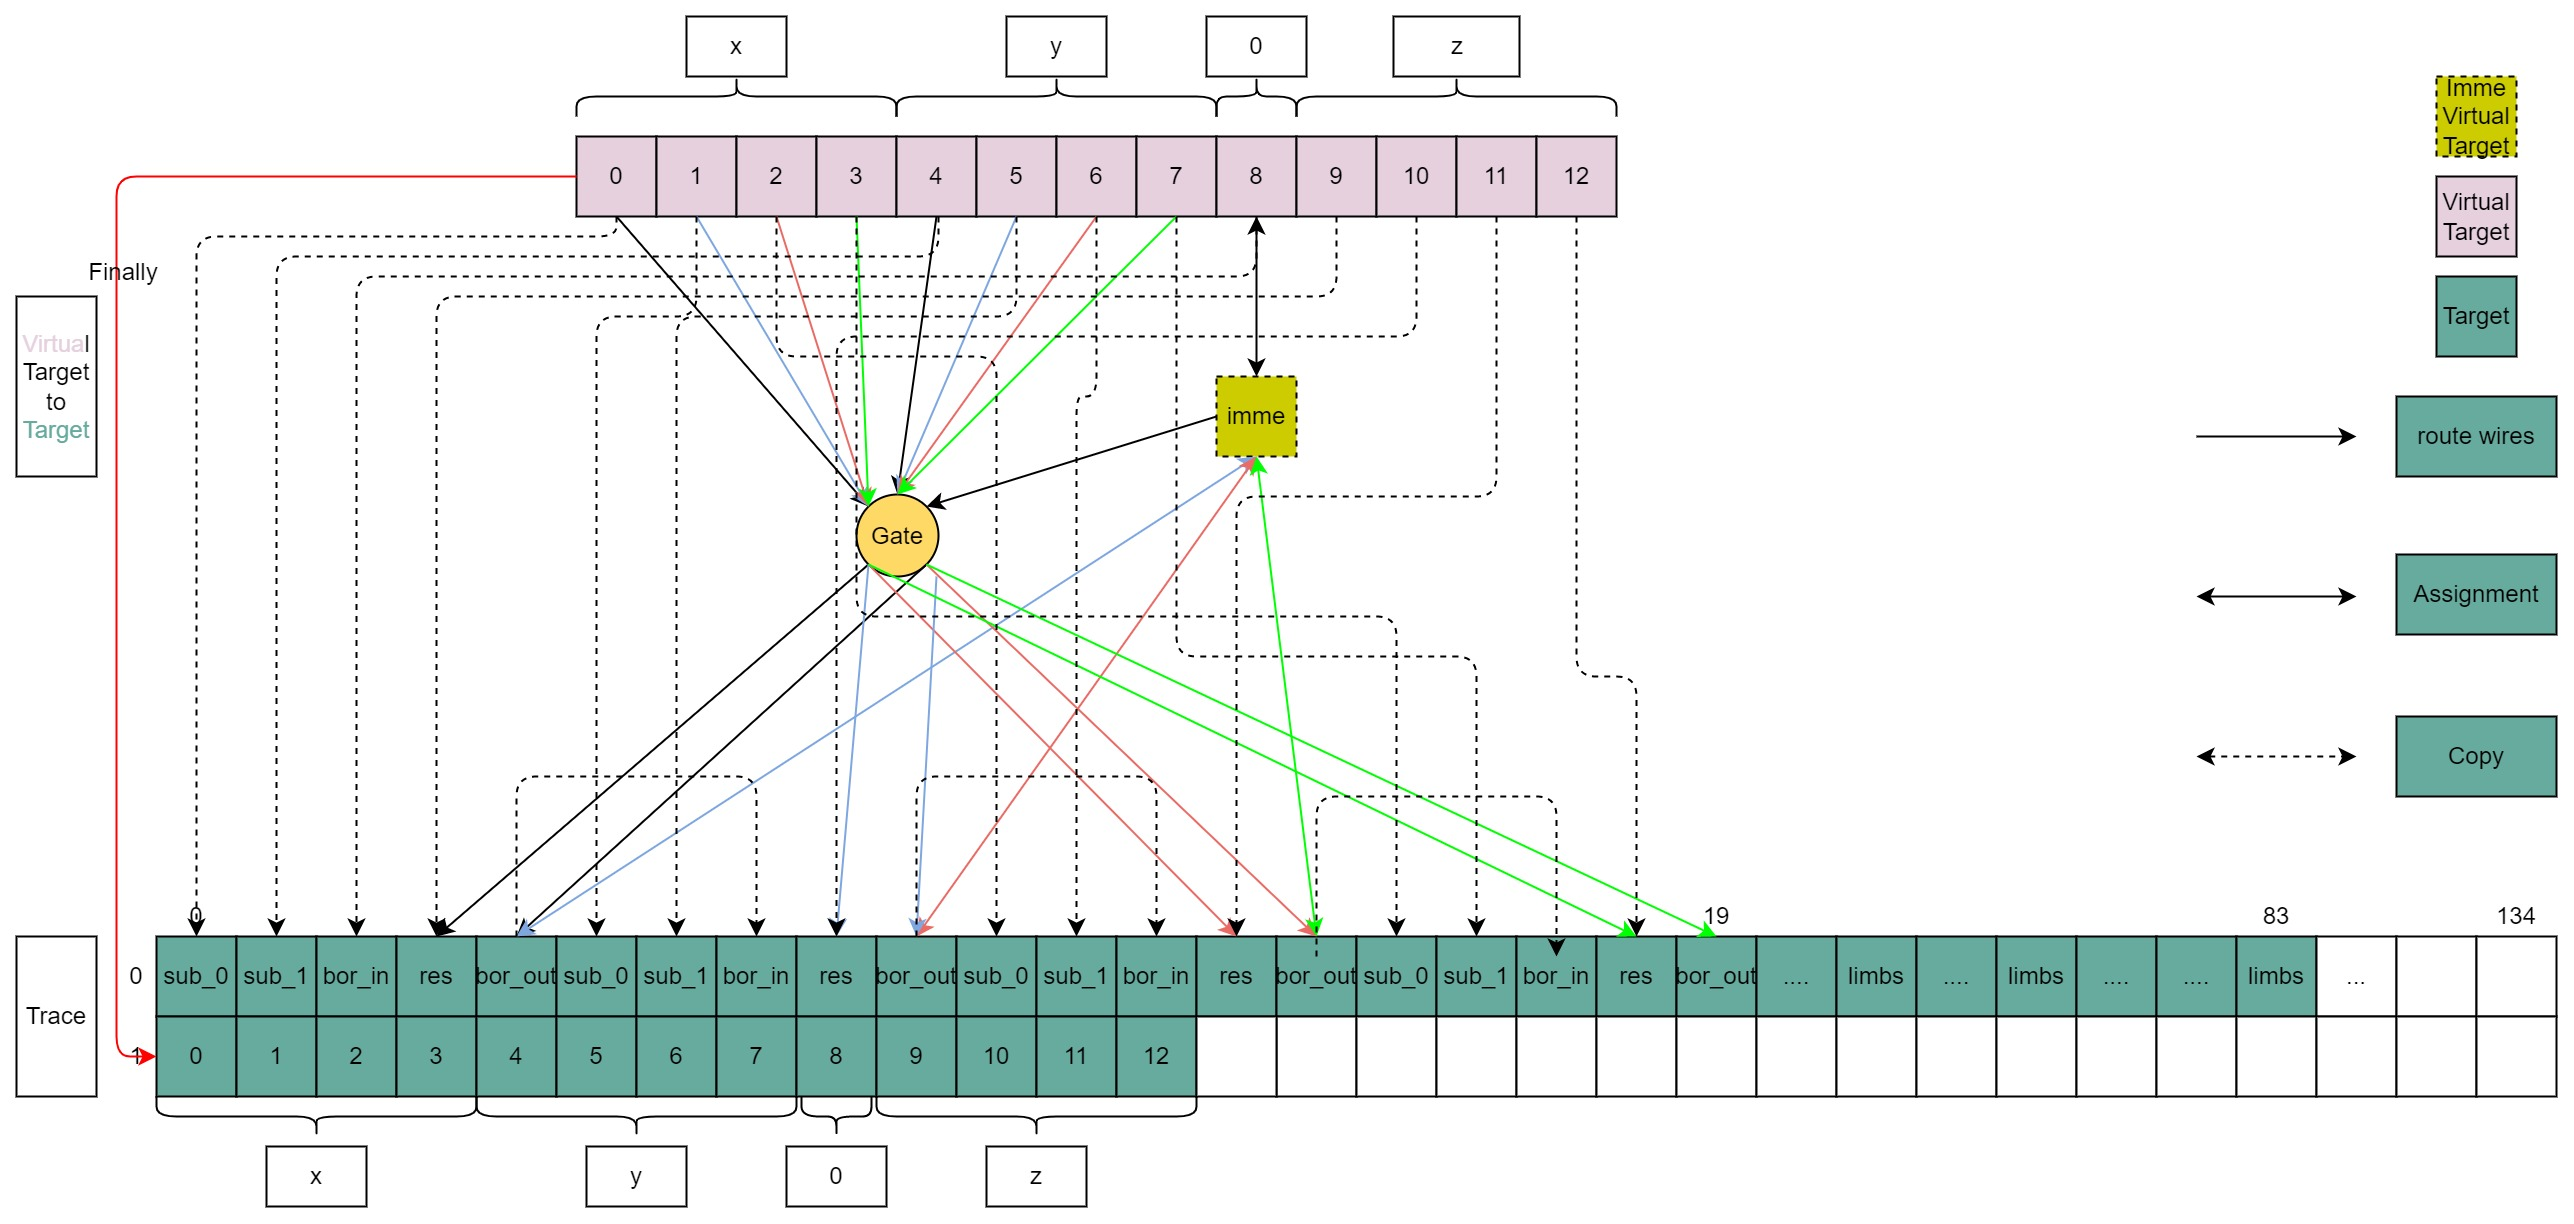
\includegraphics[width=0.6\textwidth]{biguint-sub-trace-layout.jpg}
    \caption{biguint-sub trace layout}
    \label{fig:biguint-sub-trace-layout}
\end{figure}
\paragraph{biguint-mul}

\begin{enumerate}
    \item \verb|Target|: Implement the multiplication of two biguints.
    \item \verb|Constraints logic|:
    \begin{itemize}
        \item Compute mul-factors first, use U32ArithmeticGate;
        \item Add mul-factors from low bits, use U32AddManyGate.
    \end{itemize}
    \item \verb|Process layout|: See \figref{fig:biguint-mul-layout}
    \item \verb|Constraints info and costs|:
    \begin{itemize}
        \item Gate type num: 4 (U32ArithmeticGate, U32AddManyGate(num-addends: 4), U32AddManyGate(num-addends: 6), U32AddManyGate(num-addends: 8))
        \item Gate instance num: 9
        \item U32ArithmeticGate num: 6
        \item U32AddManyGate num: 3
        \item copy-constraints: $18 \times 3 + (4 + 6 + 8) \times 2 + 9 = 99$
        \item max-degree: 4
    \end{itemize}
\end{enumerate}

\begin{figure}[!ht]
    \centering
    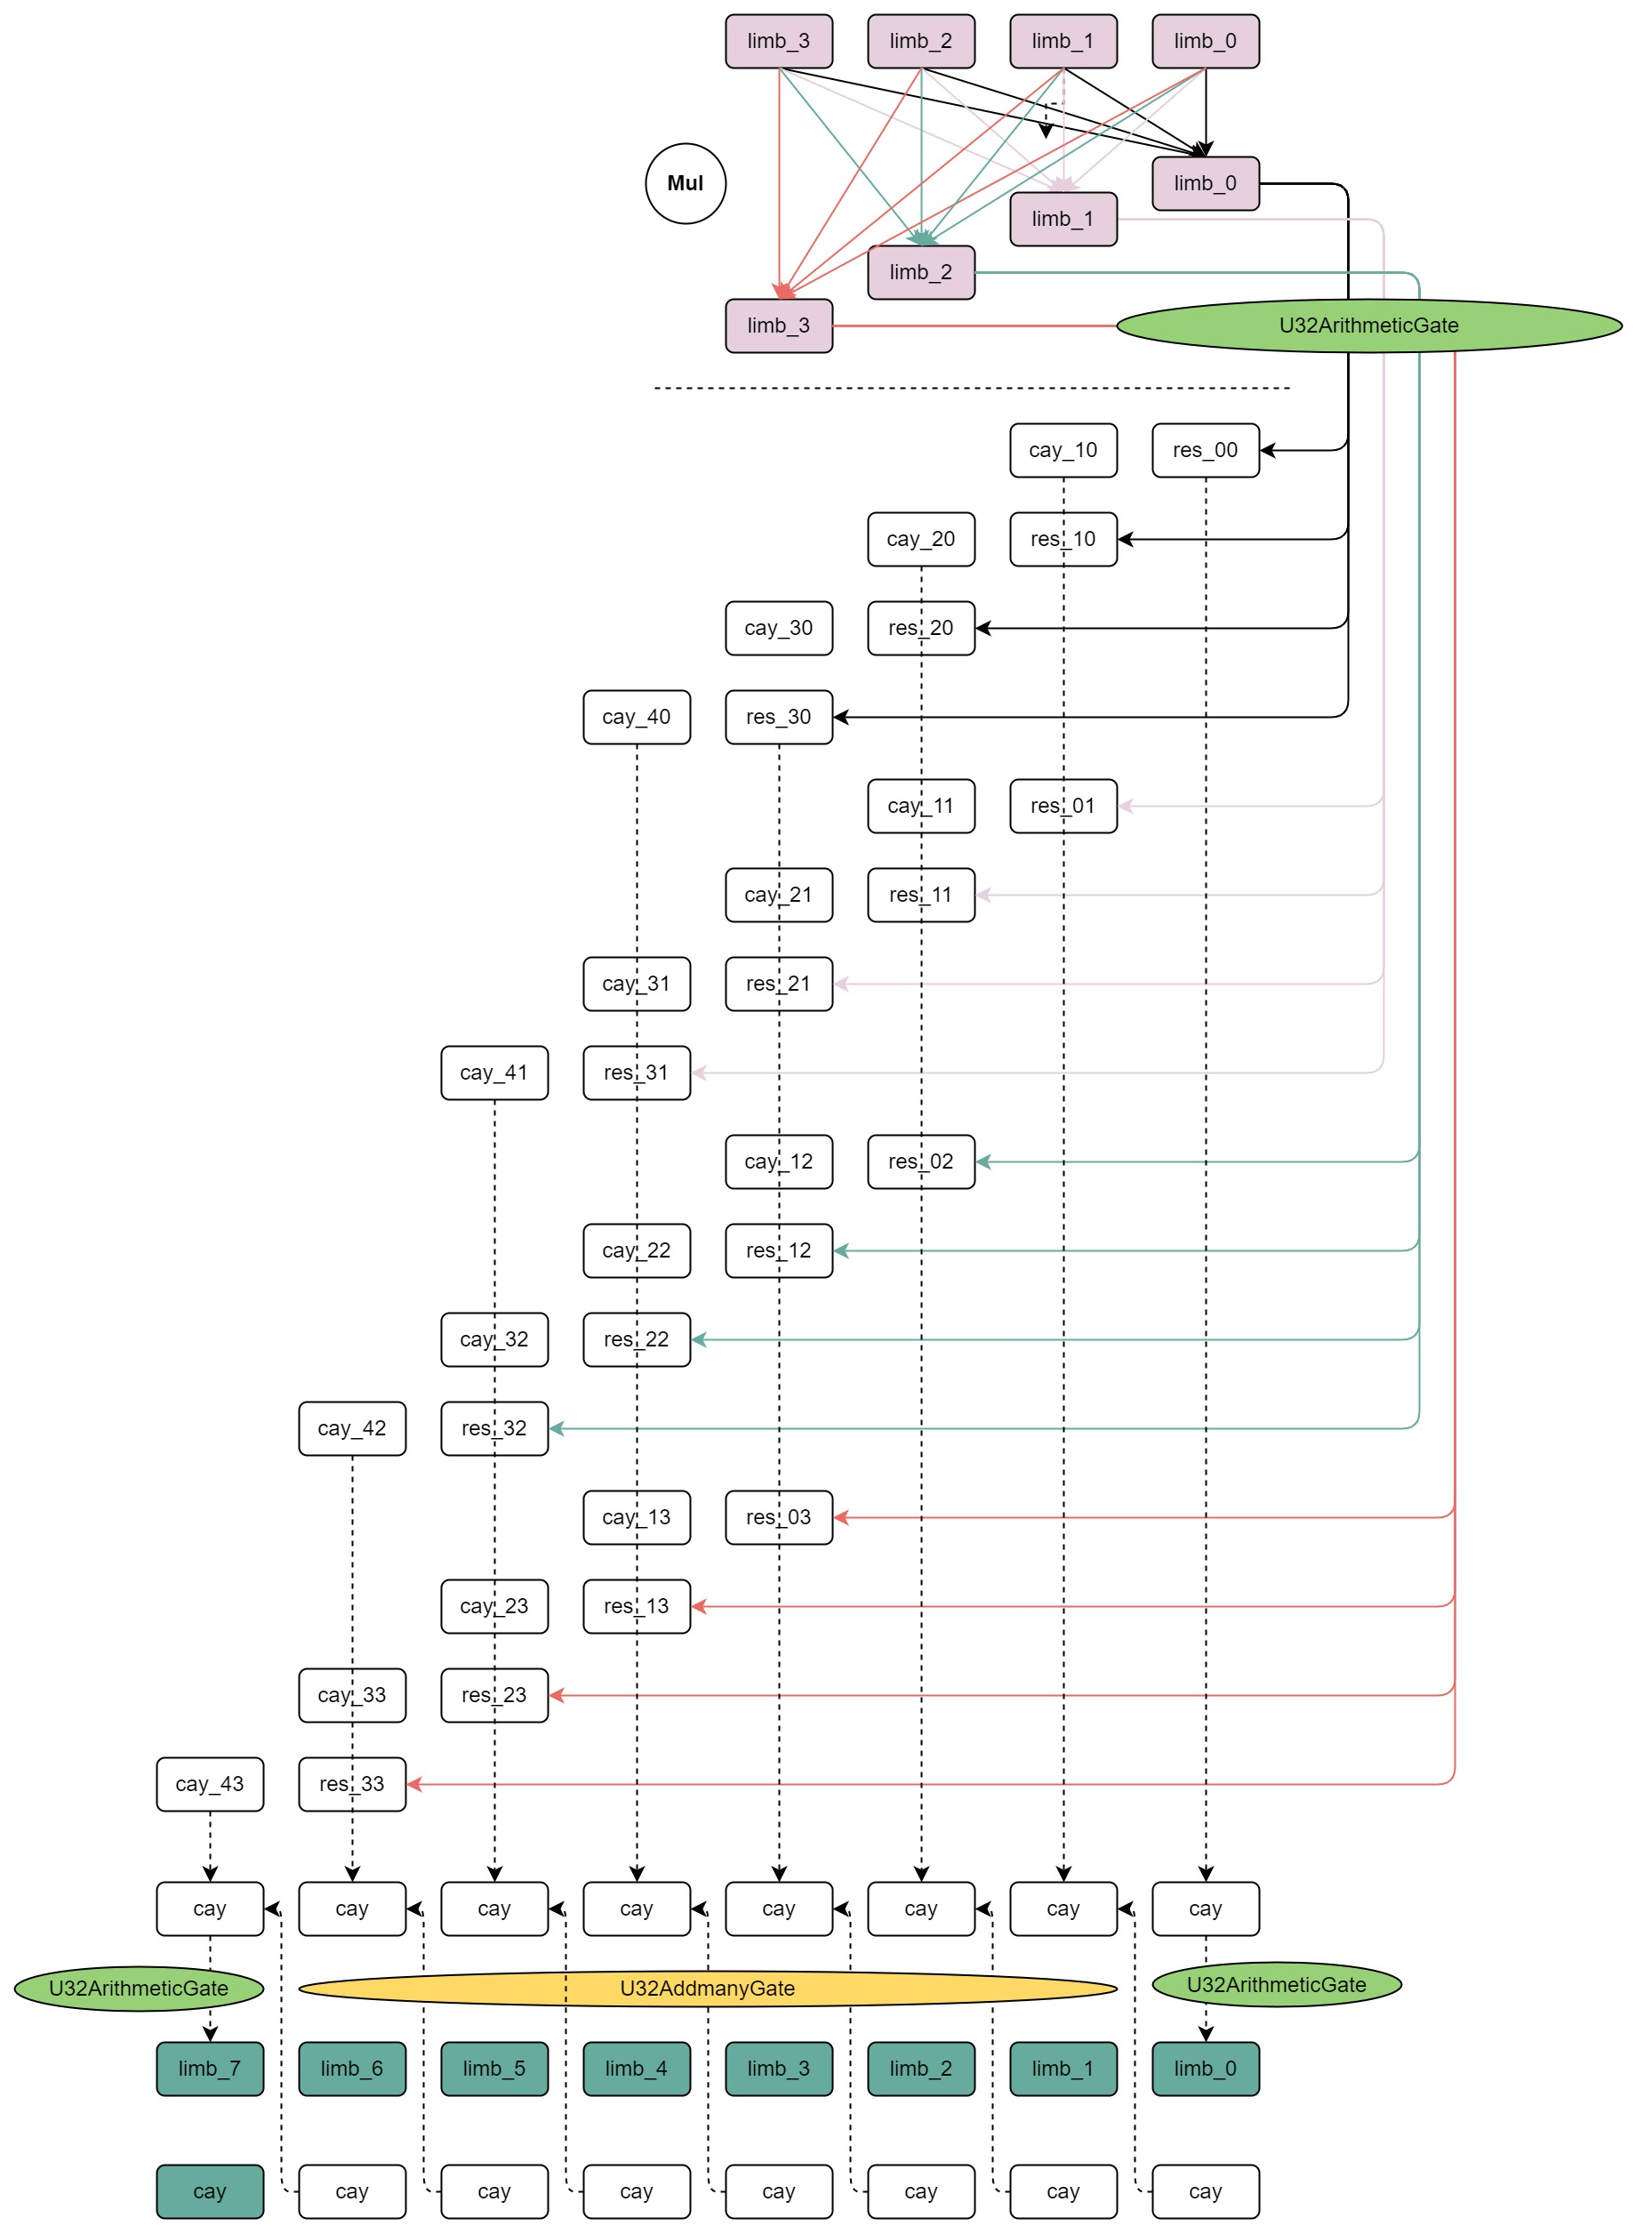
\includegraphics[width=0.6\textwidth]{biguint-mul-layout.jpg}
    \caption{biguint-mul layout}
    \label{fig:biguint-mul-layout}
\end{figure}
\paragraph{biguint-div}

Note that div-rem has the same constraints logic with div

\subparagraph{Target}
Implement the division of two biguints.

\subparagraph{Constraints logic}
\begin{itemize}
    \item Not implement div-algrithem directly;
    \item Use nondeterministic feature to check div-logic;
    \item Check \verb|div * b + rem = a|;
    \item Check \verb|rem < b|.
\end{itemize}

\subparagraph{Process layout}
See \figref{fig:biguint-div-layout}.
\begin{figure}[!ht]
    \centering
    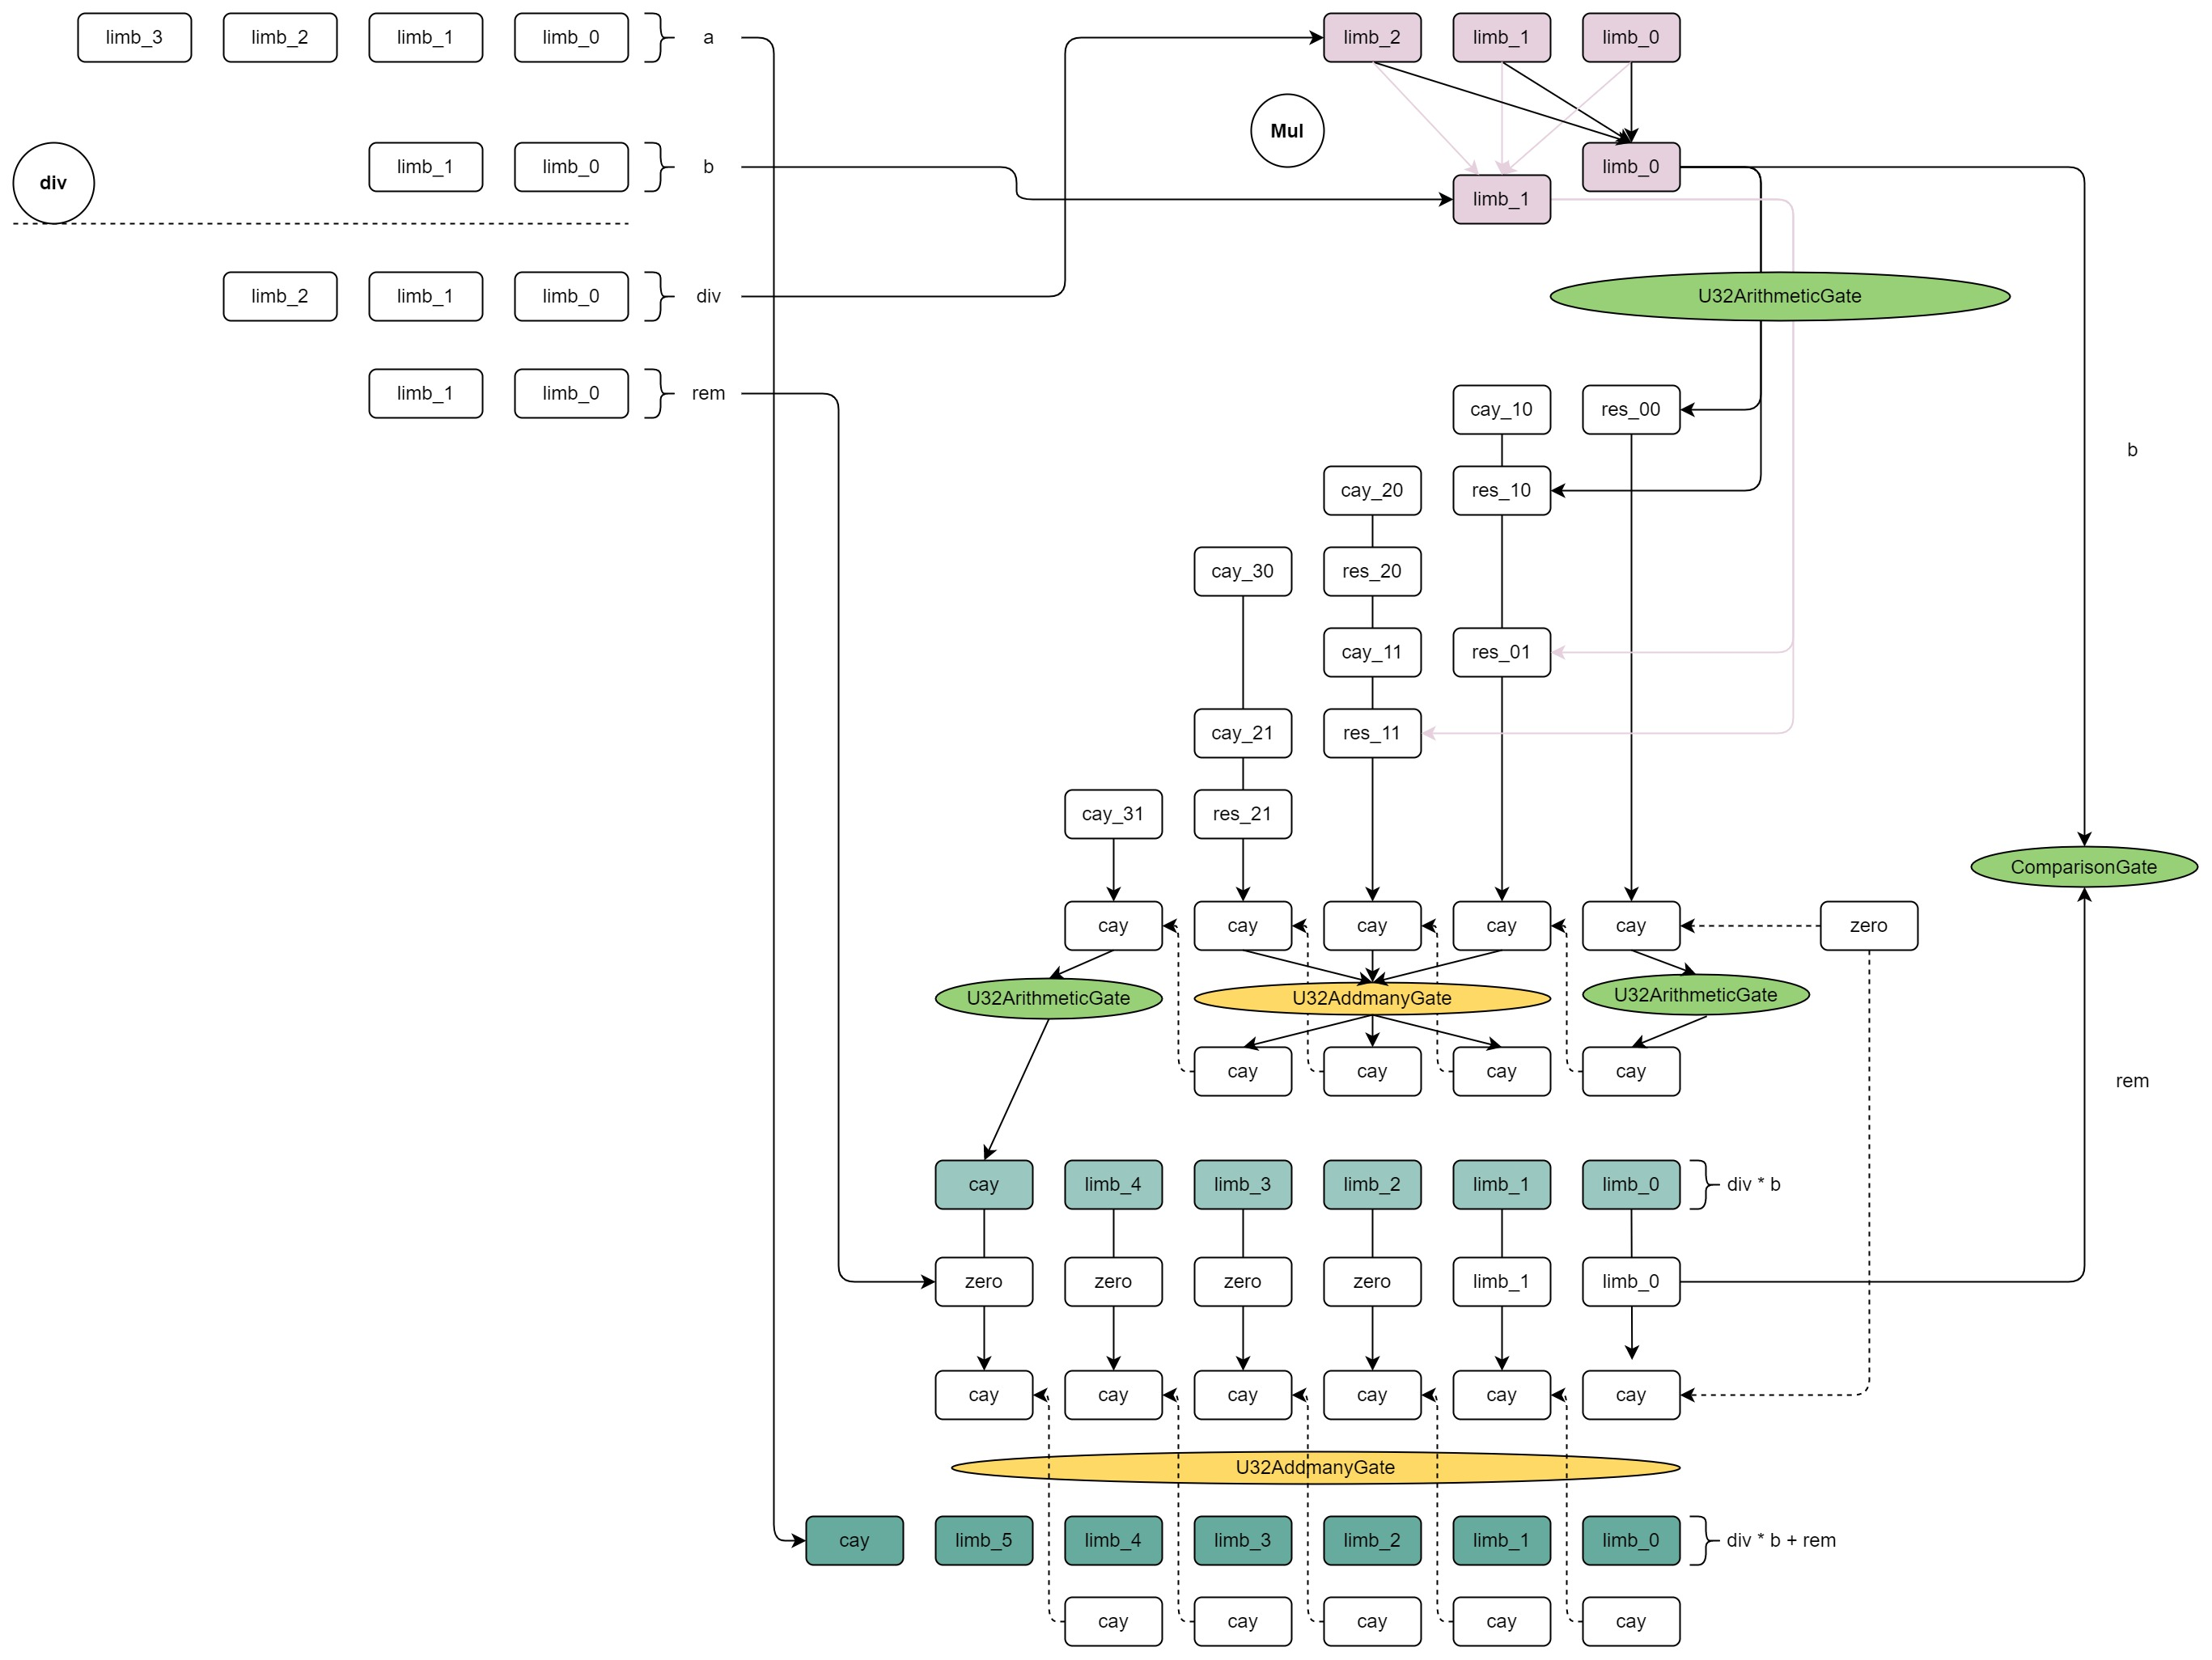
\includegraphics[width=0.8\textwidth]{biguint-div-layout.jpg}
    \caption{biguint-div layout}
    \label{fig:biguint-div-layout}
\end{figure}

\subparagraph{Constraints info and costs}
\begin{itemize}
    \item Gate type num: 5 (U32ArithmeticGate, U32AddManyGate(num-addends: 3), U32AddManyGate(num-addends: 4), ComparisionGate, ArithmeticGate)
    \item Gate instance num: $3 + 3 + 4 + 3 = 13$
    \item U32ArithmeticGate num: 3
    \item U32AddManyGate num: 3
    \item ComparisionGate num: 4
    \item ArithmeticGate num: 3
    \item copy-constraints: $3 \times 8 + 4 + 5 + 4 + 4 \times 6 + 7 + 1 + 26 + 5 = 100$
    \item max-degree: 4
\end{itemize}

\subsubsubsection{biguint-cmp}
{biguint-cmp}

\begin{enumerate}
    \item \verb|Target|: Implement the comparison of two biguints.
    \item \verb|Constraints logic|
    \begin{itemize}
        \item Split the input to many limbs, such that: \verb|limbs_num = bits / chunks|;
        \item Execute comparison for low bits limbs;
        \item Ensure that the result is determined by the highest limbs which are not equal.
    \end{itemize}
    \item \verb|Process layout|: See \ref{fig:biguint-cmp-layout}.
    \item \verb|Circuit layout|: See \ref{fig:biguint-cmp-circuit-layout}.
    \item \verb|Constraints info and costs|:
    \begin{itemize}
        \item Gate type num: 2 (ComparisionGate, ArithmeticGate)
        \item Gate instance num: $4 \times 2 + 3 = 11$
        \item ComparisionGate num: 8
        \item ArithmeticGate num: 3
        \item copy-constraints: $(4 + 9) \times 4 + 1 = 53$
        \item max-degree: 4
    \end{itemize}
\end{enumerate}

\begin{figure}[!ht]
    \centering
    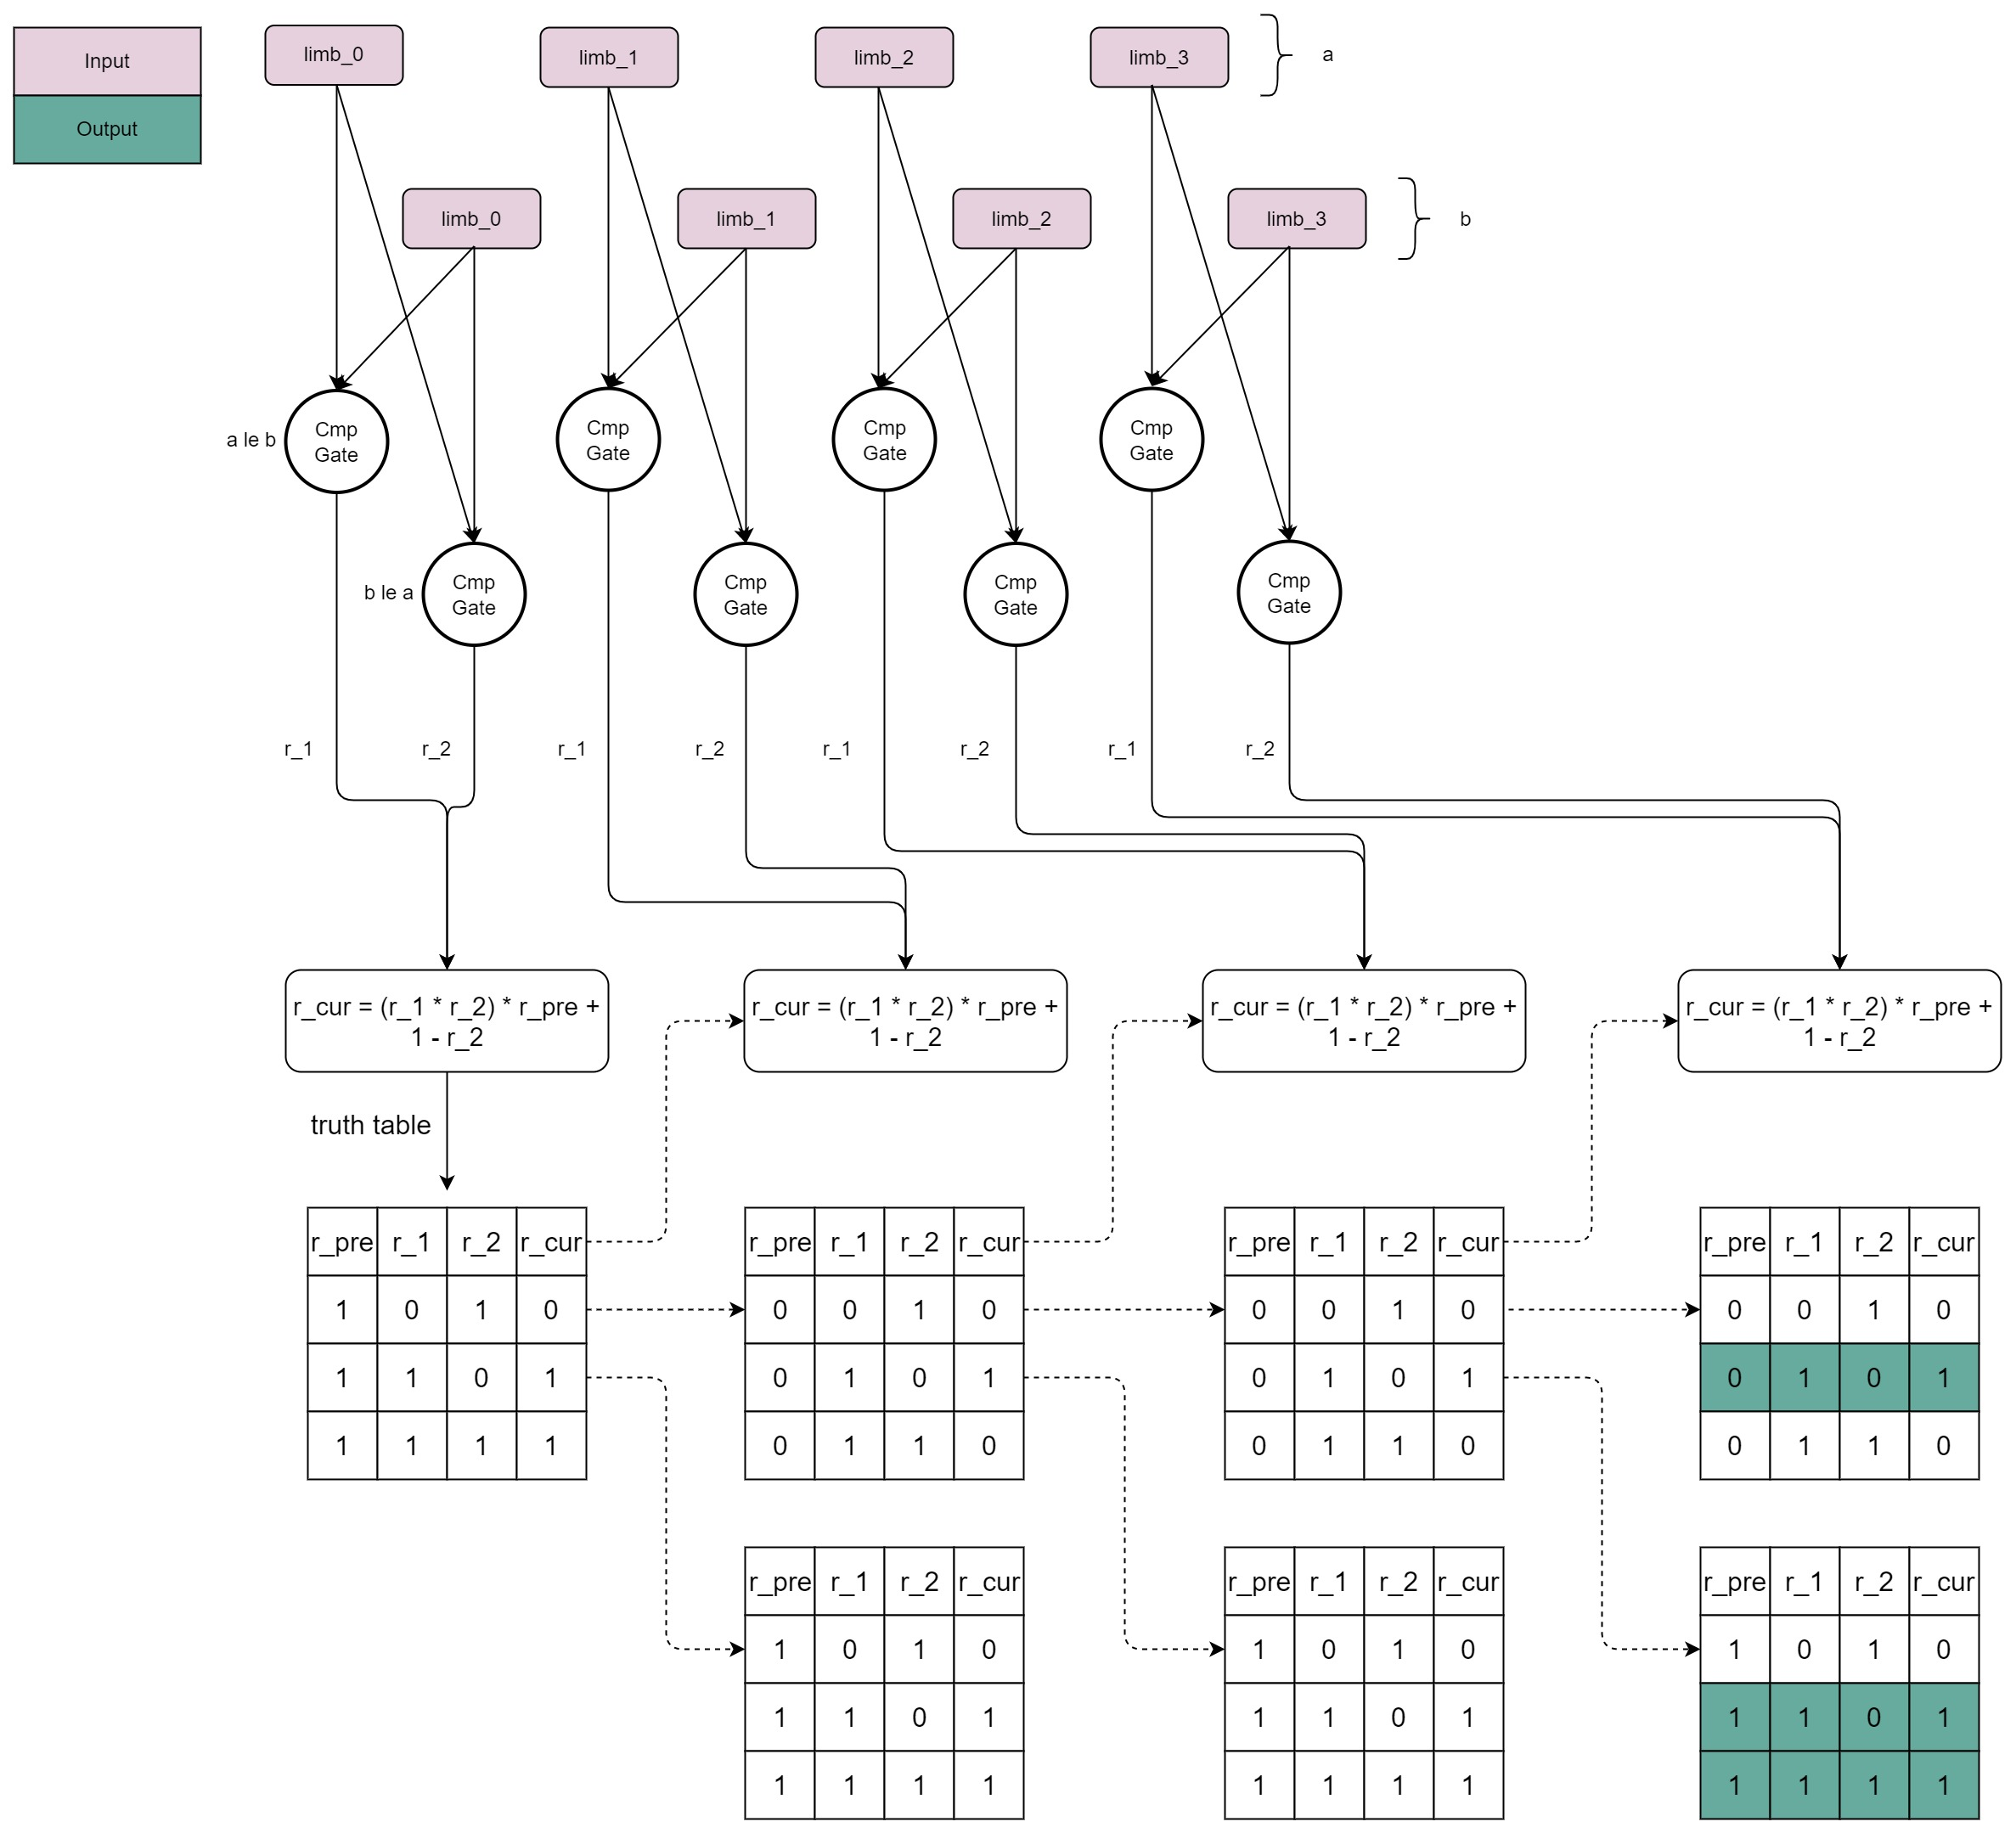
\includegraphics[width=0.6\textwidth]{biguint-cmp-layout.jpg}
    \caption{biguint-cmp layout}
    \label{fig:biguint-cmp-layout}
\end{figure}

\begin{figure}[!ht]
    \centering
    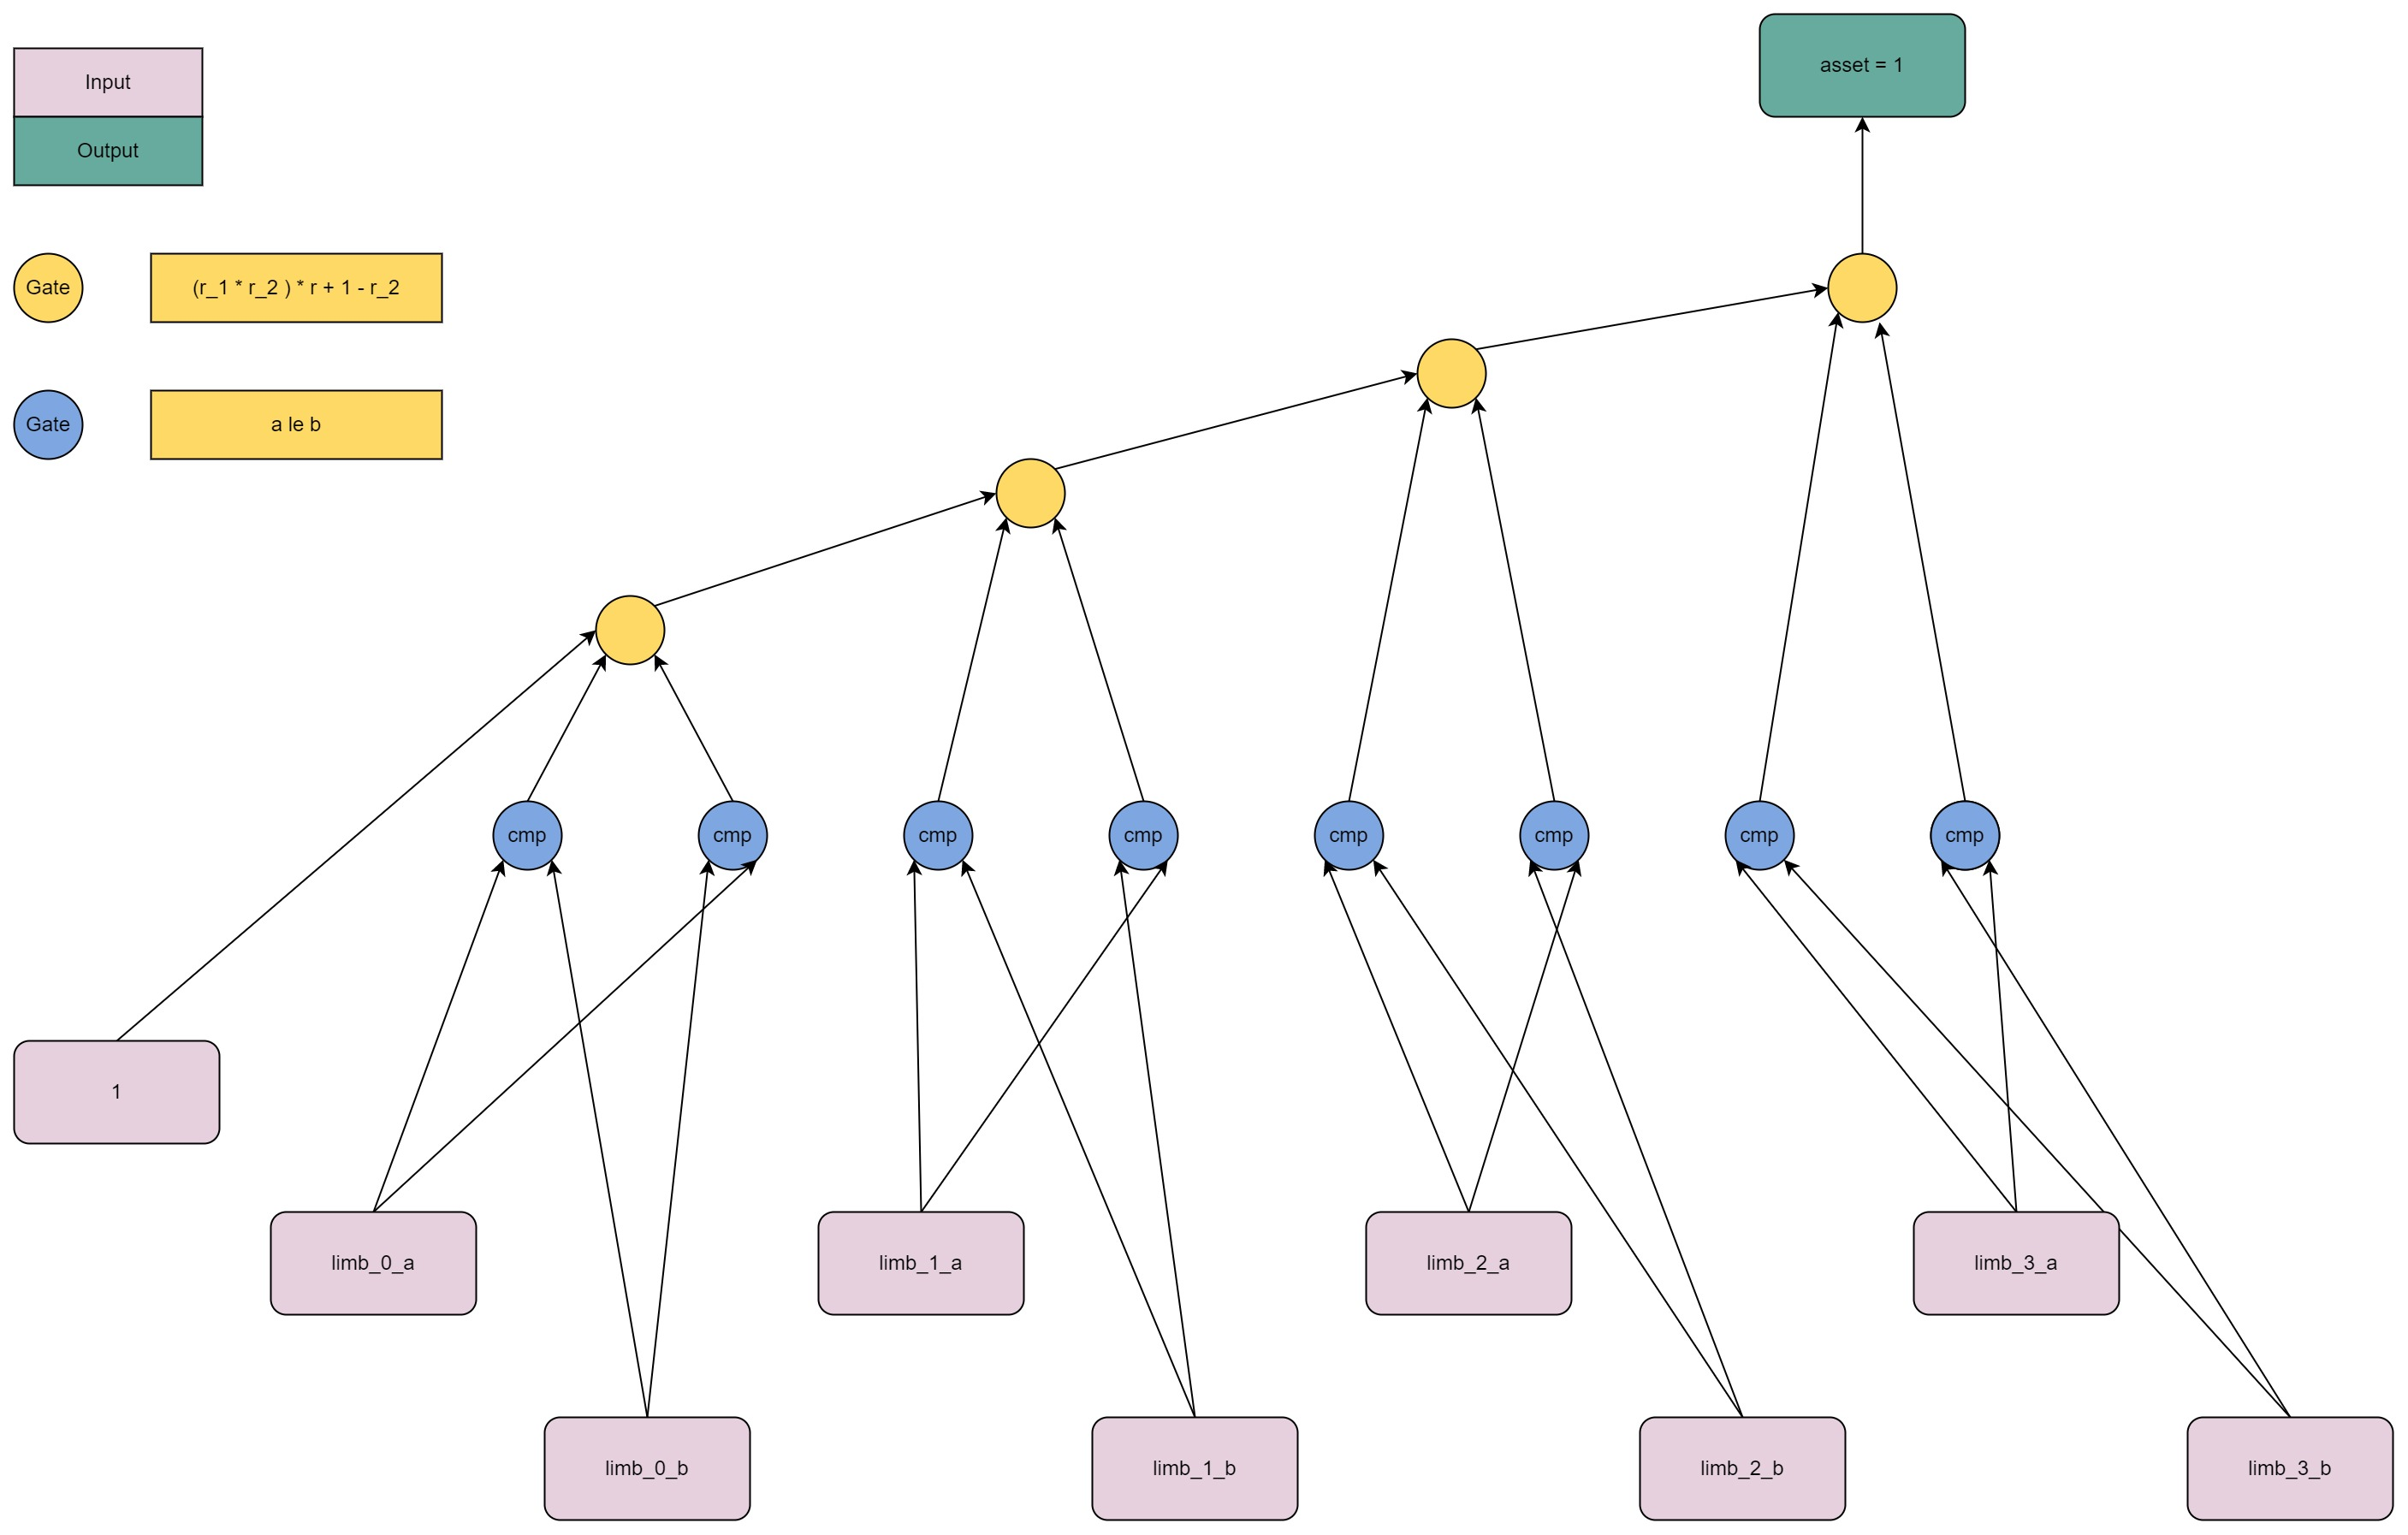
\includegraphics[width=0.6\textwidth]{biguint-cmp-circuit-layout.jpg}
    \caption{biguint-cmp circuit layout}
    \label{fig:biguint-cmp-circuit-layout}
\end{figure}

\subsubsubsection{non-native-add}

\begin{enumerate}
    \item \verb|Target|: Check the additional relation among three non-native target objects.
    \item \verb|Constraints logic|:
    \begin{itemize}
        \item Check equation for gadget: \verb|a + b = c + modular * overflow|;
        \item Check that ``c < modular''.
    \end{itemize}
    \item \verb|Process layout|: See \figref{fig:non-native-add-layout}.
    \item \verb|Constraints info and costs|:
    \begin{itemize}
        \item gadget biguint-add num: 2
        \item gadget biguint-mul-by-bool num: 1
        \item gadget biguint-cmp num: 1
        \item gate type num: 3 (U32AddManyGate, ComparisonGate, ArithmeticGate)
        \item gate instance num: 23 = 3 (U32AddManyGate) + 16 (ComparisonGate) + 2 (ArithmeticGate (1,0)) + 1 (ArithmeticGate(1,-1)) + 1 (ArithmeticGate(1,1))
        \item copy-constraints: 186 = 32 * 2{biguint-add} + 9{biguint-mul-by-bool} + 9 + (4 + 9) * 8{biguint-cmp} = 186
    \end{itemize}
\end{enumerate}

\begin{figure}[!ht]
    \centering
    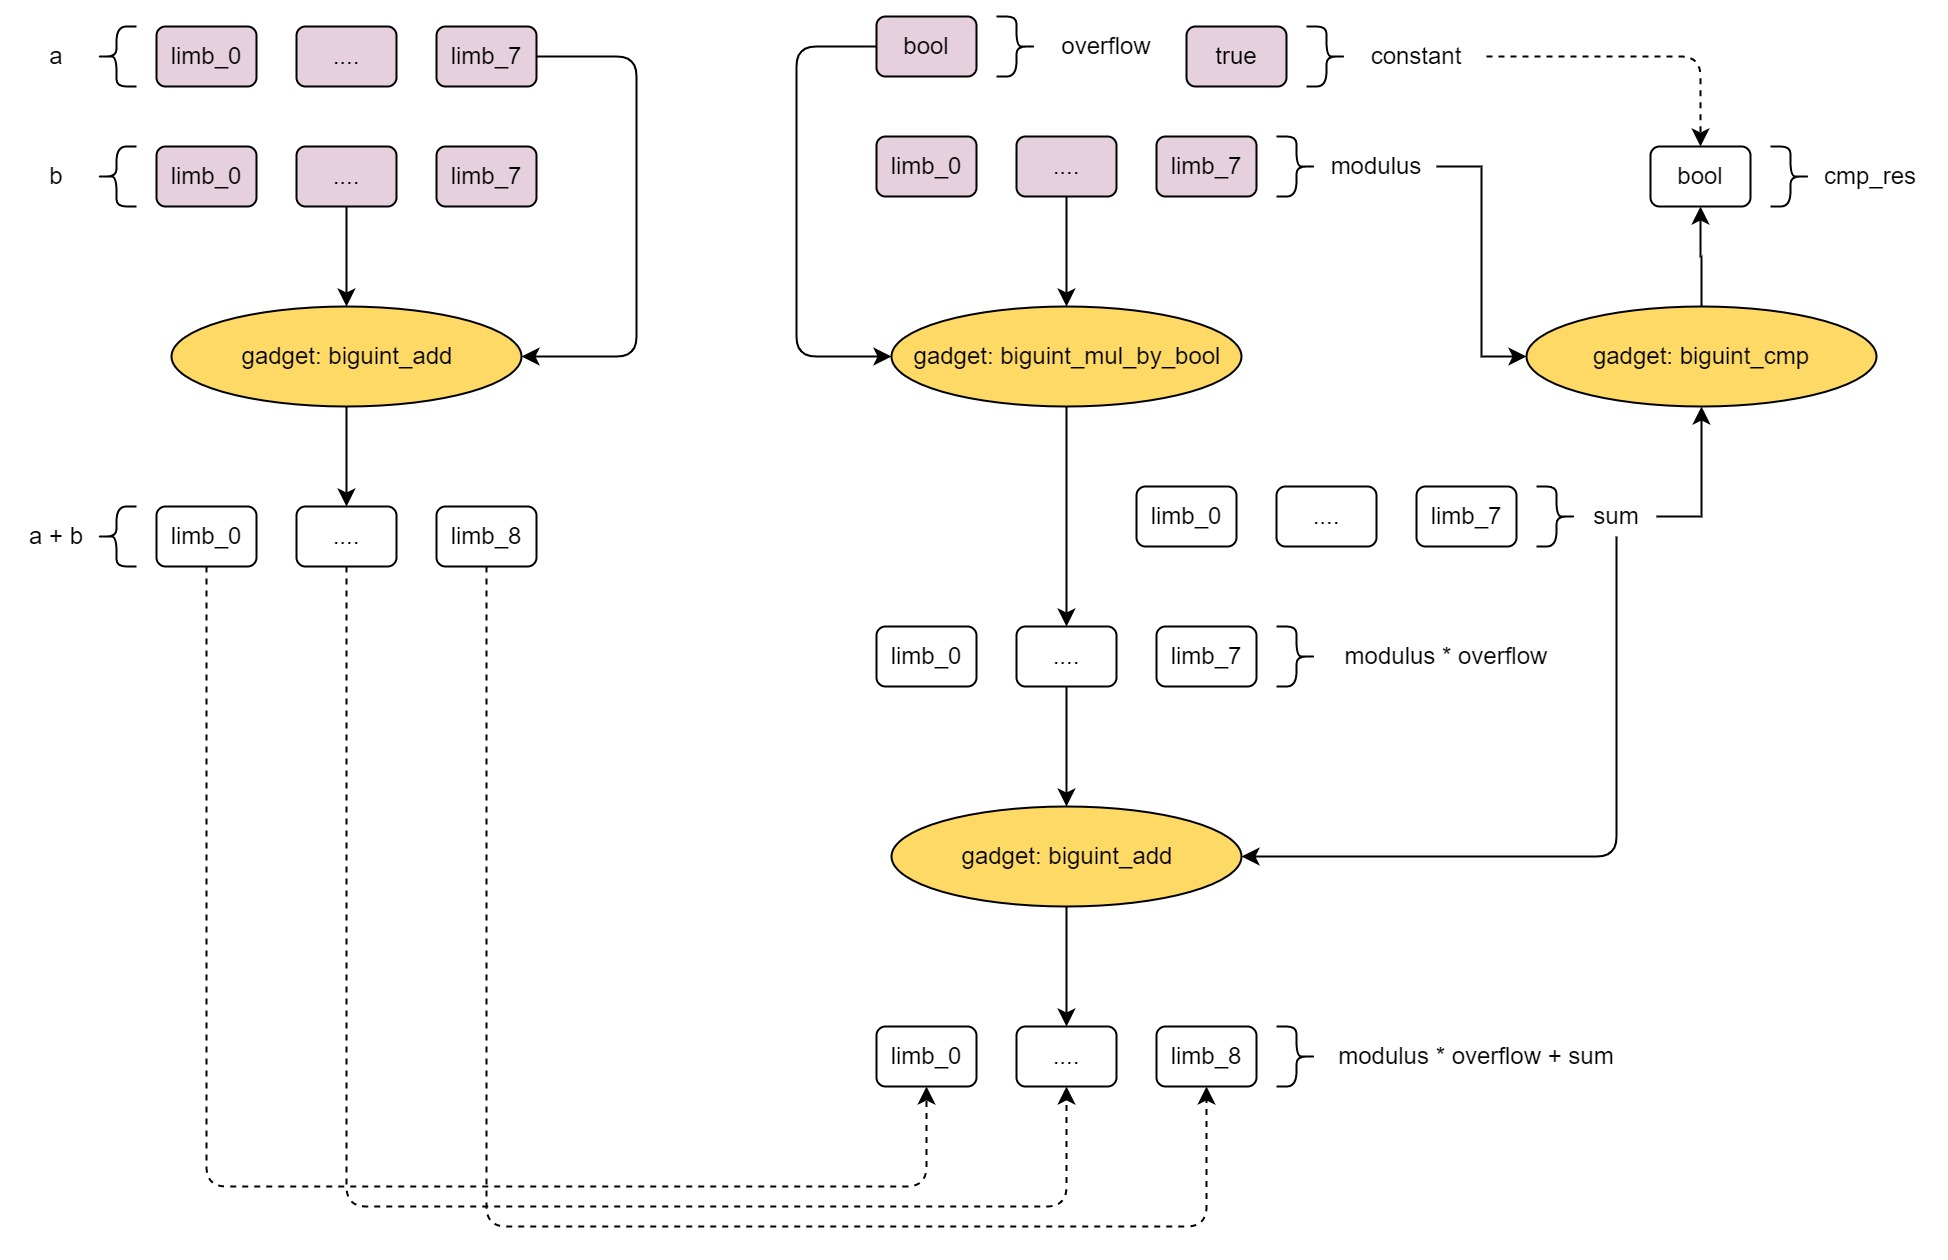
\includegraphics[width=0.6\textwidth]{nonnative-add-layout.jpg}
    \caption{non-native-add layout}
    \label{fig:non-native-add-layout}
\end{figure}

\paragraph{non-native-sub}

\begin{enumerate}
    \item \verb|Target|: Check the substrate relation among three non-native target objects.
    \item \verb|Constraints logic|:
    \begin{itemize}
        \item Check equation for gadget: \verb|diff + b = a + modular * overflow|;
        \item Check that ``overflow is bool'';
        \item Check that ``diff.limbs is range U32''.
    \end{itemize}
    \item \verb|Process layout|: See \figref{fig:non-native-sub-layout}
    \item \verb|Constraints info and costs|:
    \begin{itemize}
        \item gadget biguint-add num: 1
        \item gadget biguint-sub num: 1
        \item gadget biguint-mul-by-bool num: 1
        \item gadget u32rangecheck num: 1
        \item gadget assert-bool num: 1
        \item gate type num: 4 (U32AddManyGate, U32SubtractionGate, U32RangeCheckGate, ArithmeticGate)
        \item gate instance num: 7 = 2 (U32AddManyGate) + 2 (U32SubtractionGate) + 1 (U32RangeCheckGate) + 1 (ArithmeticGate(1,0)) + 1 (ArithmeticGate(1,-1))
        \item copy-constraints: 89 = 32{biguint-add num} + 27{U32SubtractionGate} + 9{biguint-mul-by-bool} + 8{u32rangecheck} + 4{assert-bool} + 9
    \end{itemize}
\end{enumerate}

\begin{figure}[!ht]
    \centering
    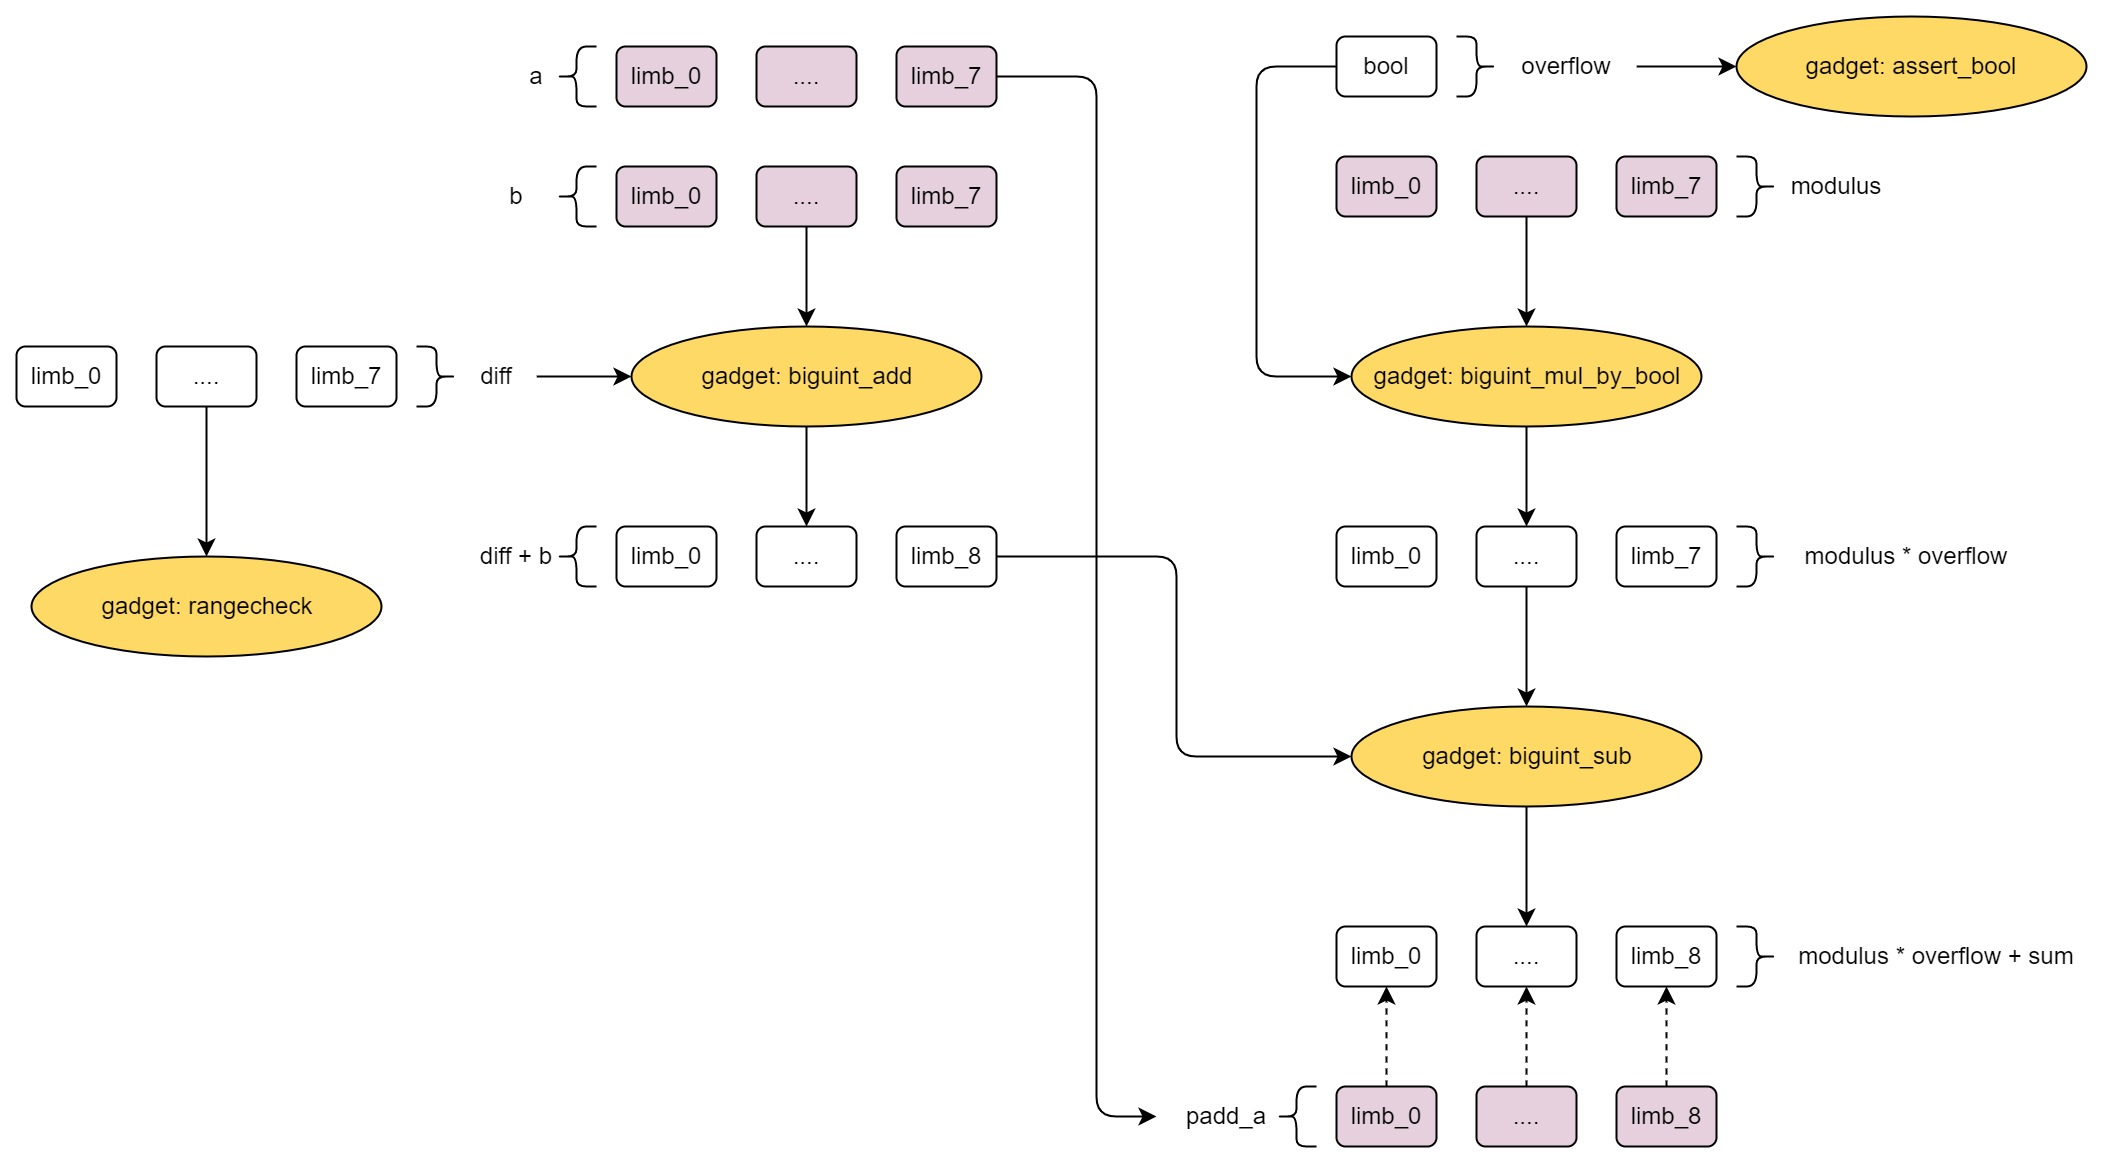
\includegraphics[width=0.6\textwidth]{nonnative-sub-layout.jpg}
    \caption{non-native-sub layout}
    \label{fig:non-native-sub-layout}
\end{figure}
\paragraph{nonnative-mul}

\subparagraph{Target}
Check the multiplication relation among three nonnative target objects.

\subparagraph{Constraints logic}
\begin{itemize}
    \item Check equation for gadget: \verb|a * b = prod + modular * overflow|;
    \item Check that ``overflow.limb is U32'';
    \item Check that ``prod.limb is U32''.
\end{itemize}

\subparagraph{Process layout}
See \figref{fig:nonnative-mul-layout}.
\begin{figure}[!ht]
    \centering
    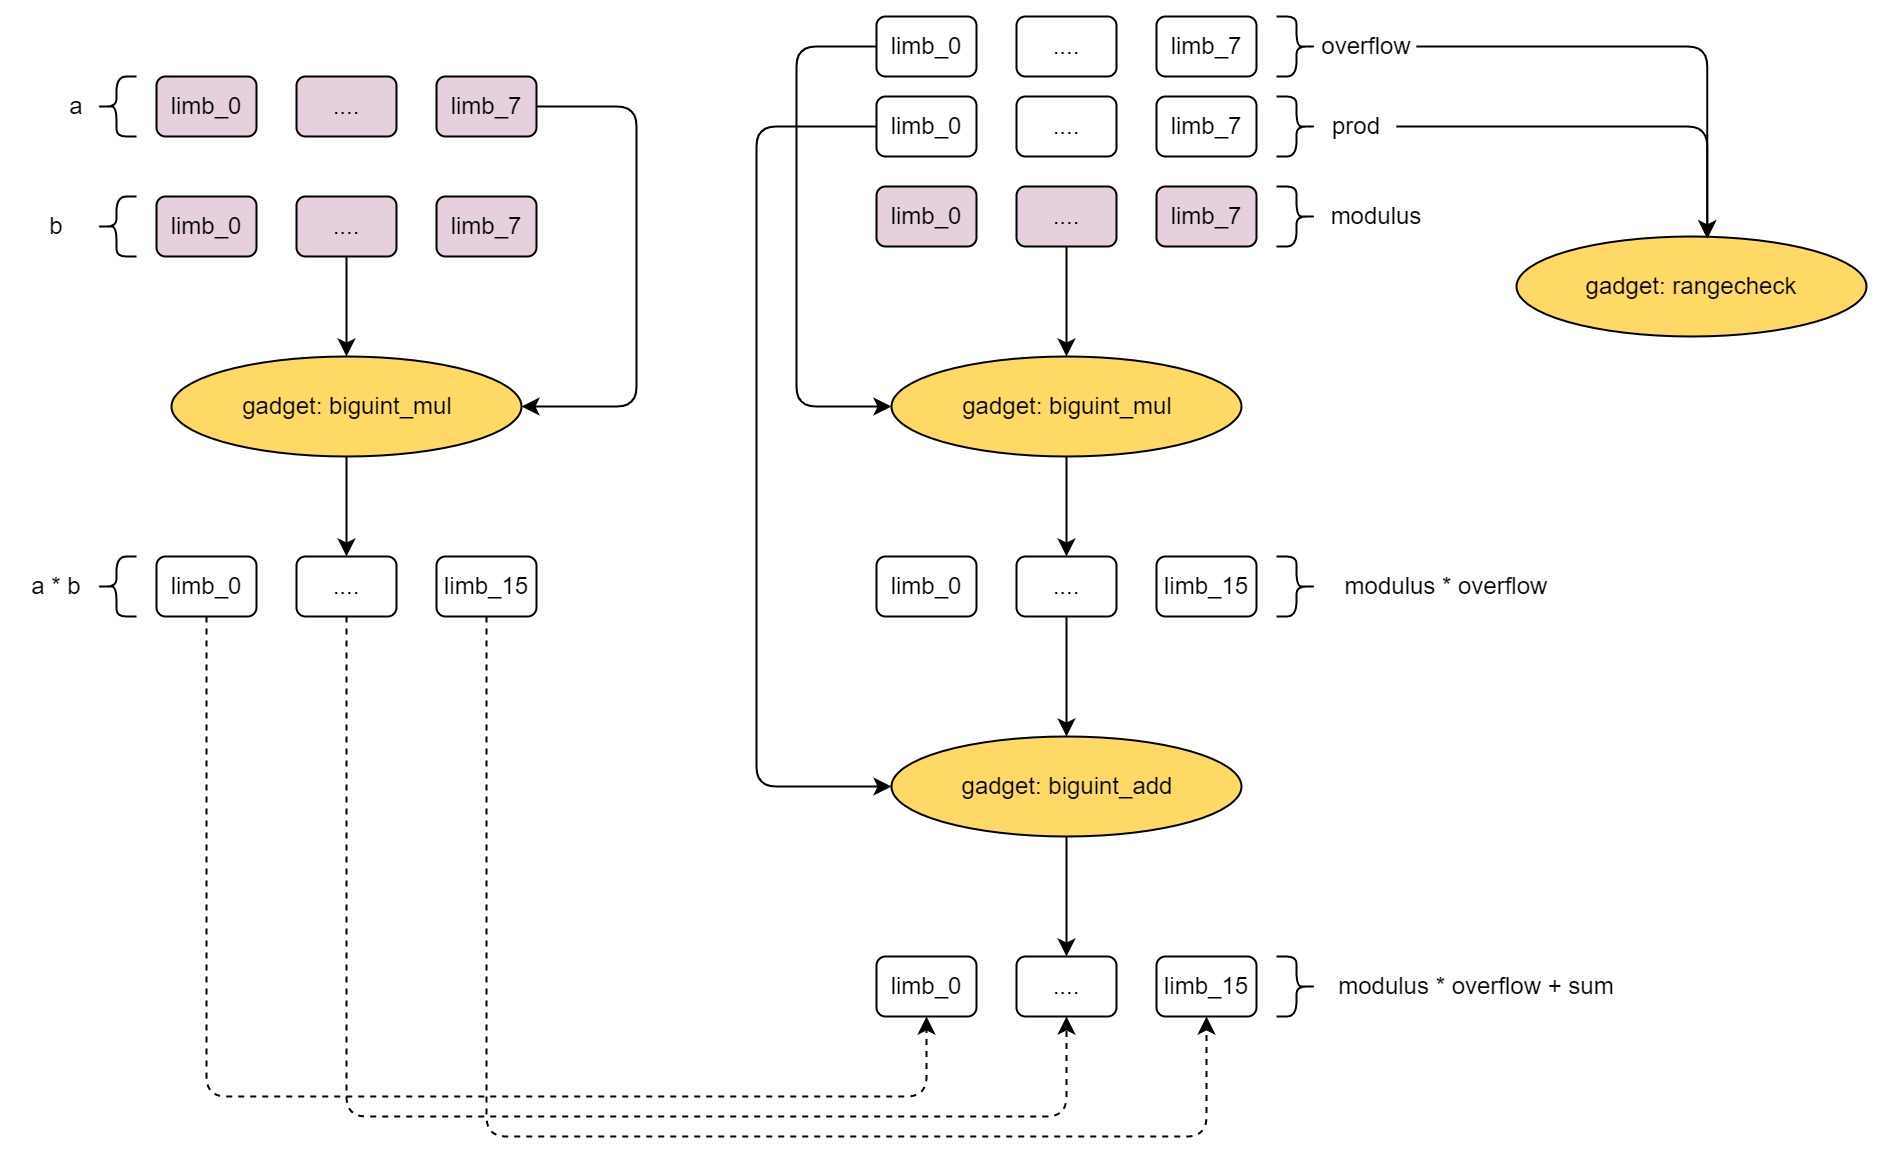
\includegraphics[width=0.6\textwidth]{nonnative-mul-layout.jpg}
    \caption{nonnative-mul layout}
    \label{fig:nonnative-mul-layout}
\end{figure}

\subparagraph{Constraints info and costs}
\begin{itemize}
    \item gadget biguint-add num: 1
    \item gadget biguint-mul num: 2
    \item gadget u32rangecheck num: 2
    \item gate type num: 9 = 7(U32AddManyGate\{3,5,7,9,11,13,15\}) + 1(U32RangeCheckGate) + 1(U32ArithmeticGate)
    \item gate instance num: 37 = 2(u32rangecheck) + 8(biguint-mul: constant-input) + 22(biguint-mul) + 1 + 3(biguint-add)
    \item copy-constraints: 583 = 8 * 2(u32rangecheck) + 3 * 3 + (4 + 6 + 8 + 10 + 12 + 14 + 16) * 4 + (8 * 8) * 3 + 17 * 4 + 18
\end{itemize}

\paragraph{nonnative-inv}

\subparagraph{Target}
Check the modular inverse relation among three nonnative target objects.

\subparagraph{Constraints logic}
\begin{itemize}
    \item Check equation for gadget: \verb|a * inv_a = 1 + modular * div|.
\end{itemize}

\subparagraph{Process layout}
See \figref{fig:nonnative-inv-layout}.
\begin{figure}[!ht]
    \centering
    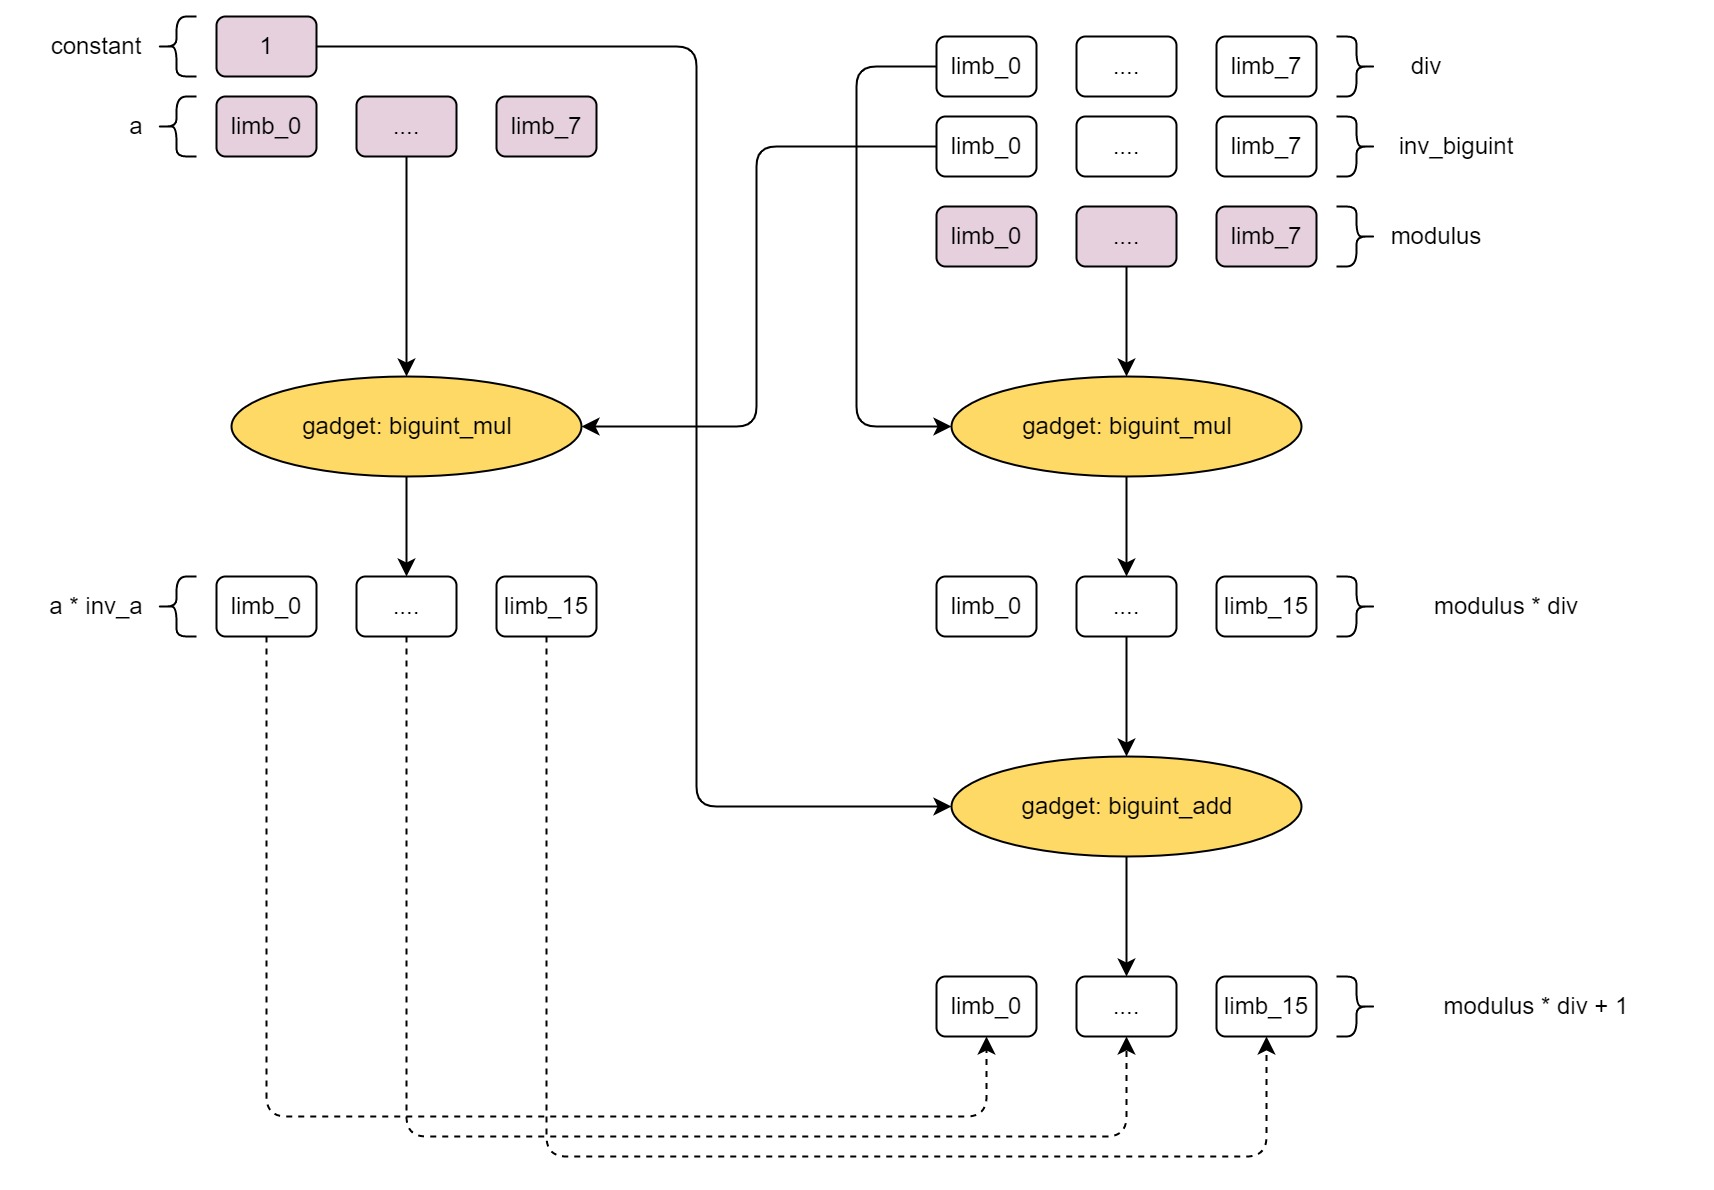
\includegraphics[width=0.8\textwidth]{nonnative-inv-layout.jpg}
    \caption{nonnative-inv layout}
    \label{fig:nonnative-inv-layout}
\end{figure}

\subparagraph{Constraints info and costs}
\begin{itemize}
    \item gadget biguint-add num: 1
    \item gadget biguint-mul num: 2
    \item gate type num: 8 = 7(U32AddManyGate\{3,5,7,9,11,13,15\}) + 1(U32ArithmeticGate)
    \item gate instance num: 56 = (8 * 8 + 2) * 2 / 3 + 5(U32AddManyGate{3}) + 5 + 2(U32AddManyGate{15})
    \item copy-constraints: 762 = (8 * 8 + 2) * 2 * 3 + 21 * 4 + (6 + 8 + 10 + 12 + 14) * 4 + 4 * 16 + 18
\end{itemize}


\paragraph{curve-add}

\subparagraph{Target}
Implement the addition of two different curve points. this is an incomplete addition, you can refer to The halo2 Book\cite{website:halo2-book} to learn more about it.

\subparagraph{Constraints logic}
$(x_1,y_1) \ne (x_2,y_2)$, See \figref{fig:curve-add}.
\begin{figure}[!ht]
    \centering
    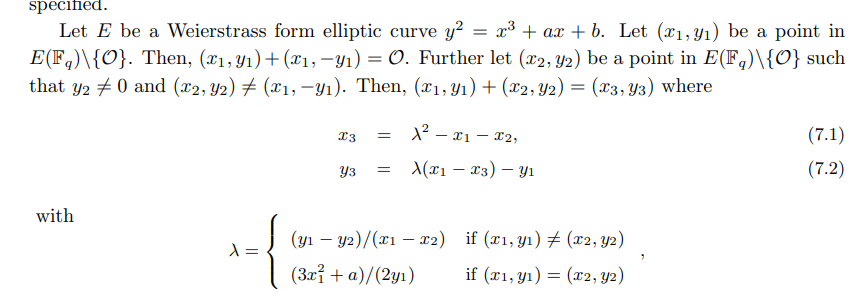
\includegraphics[width=0.6\textwidth]{curve-add.jpg}
    \caption{curve-add}
    \label{fig:curve-add}
\end{figure}

\subparagraph{Process layout}
See \figref{fig:curve-add-layout}
\begin{figure}[!ht]
    \centering
    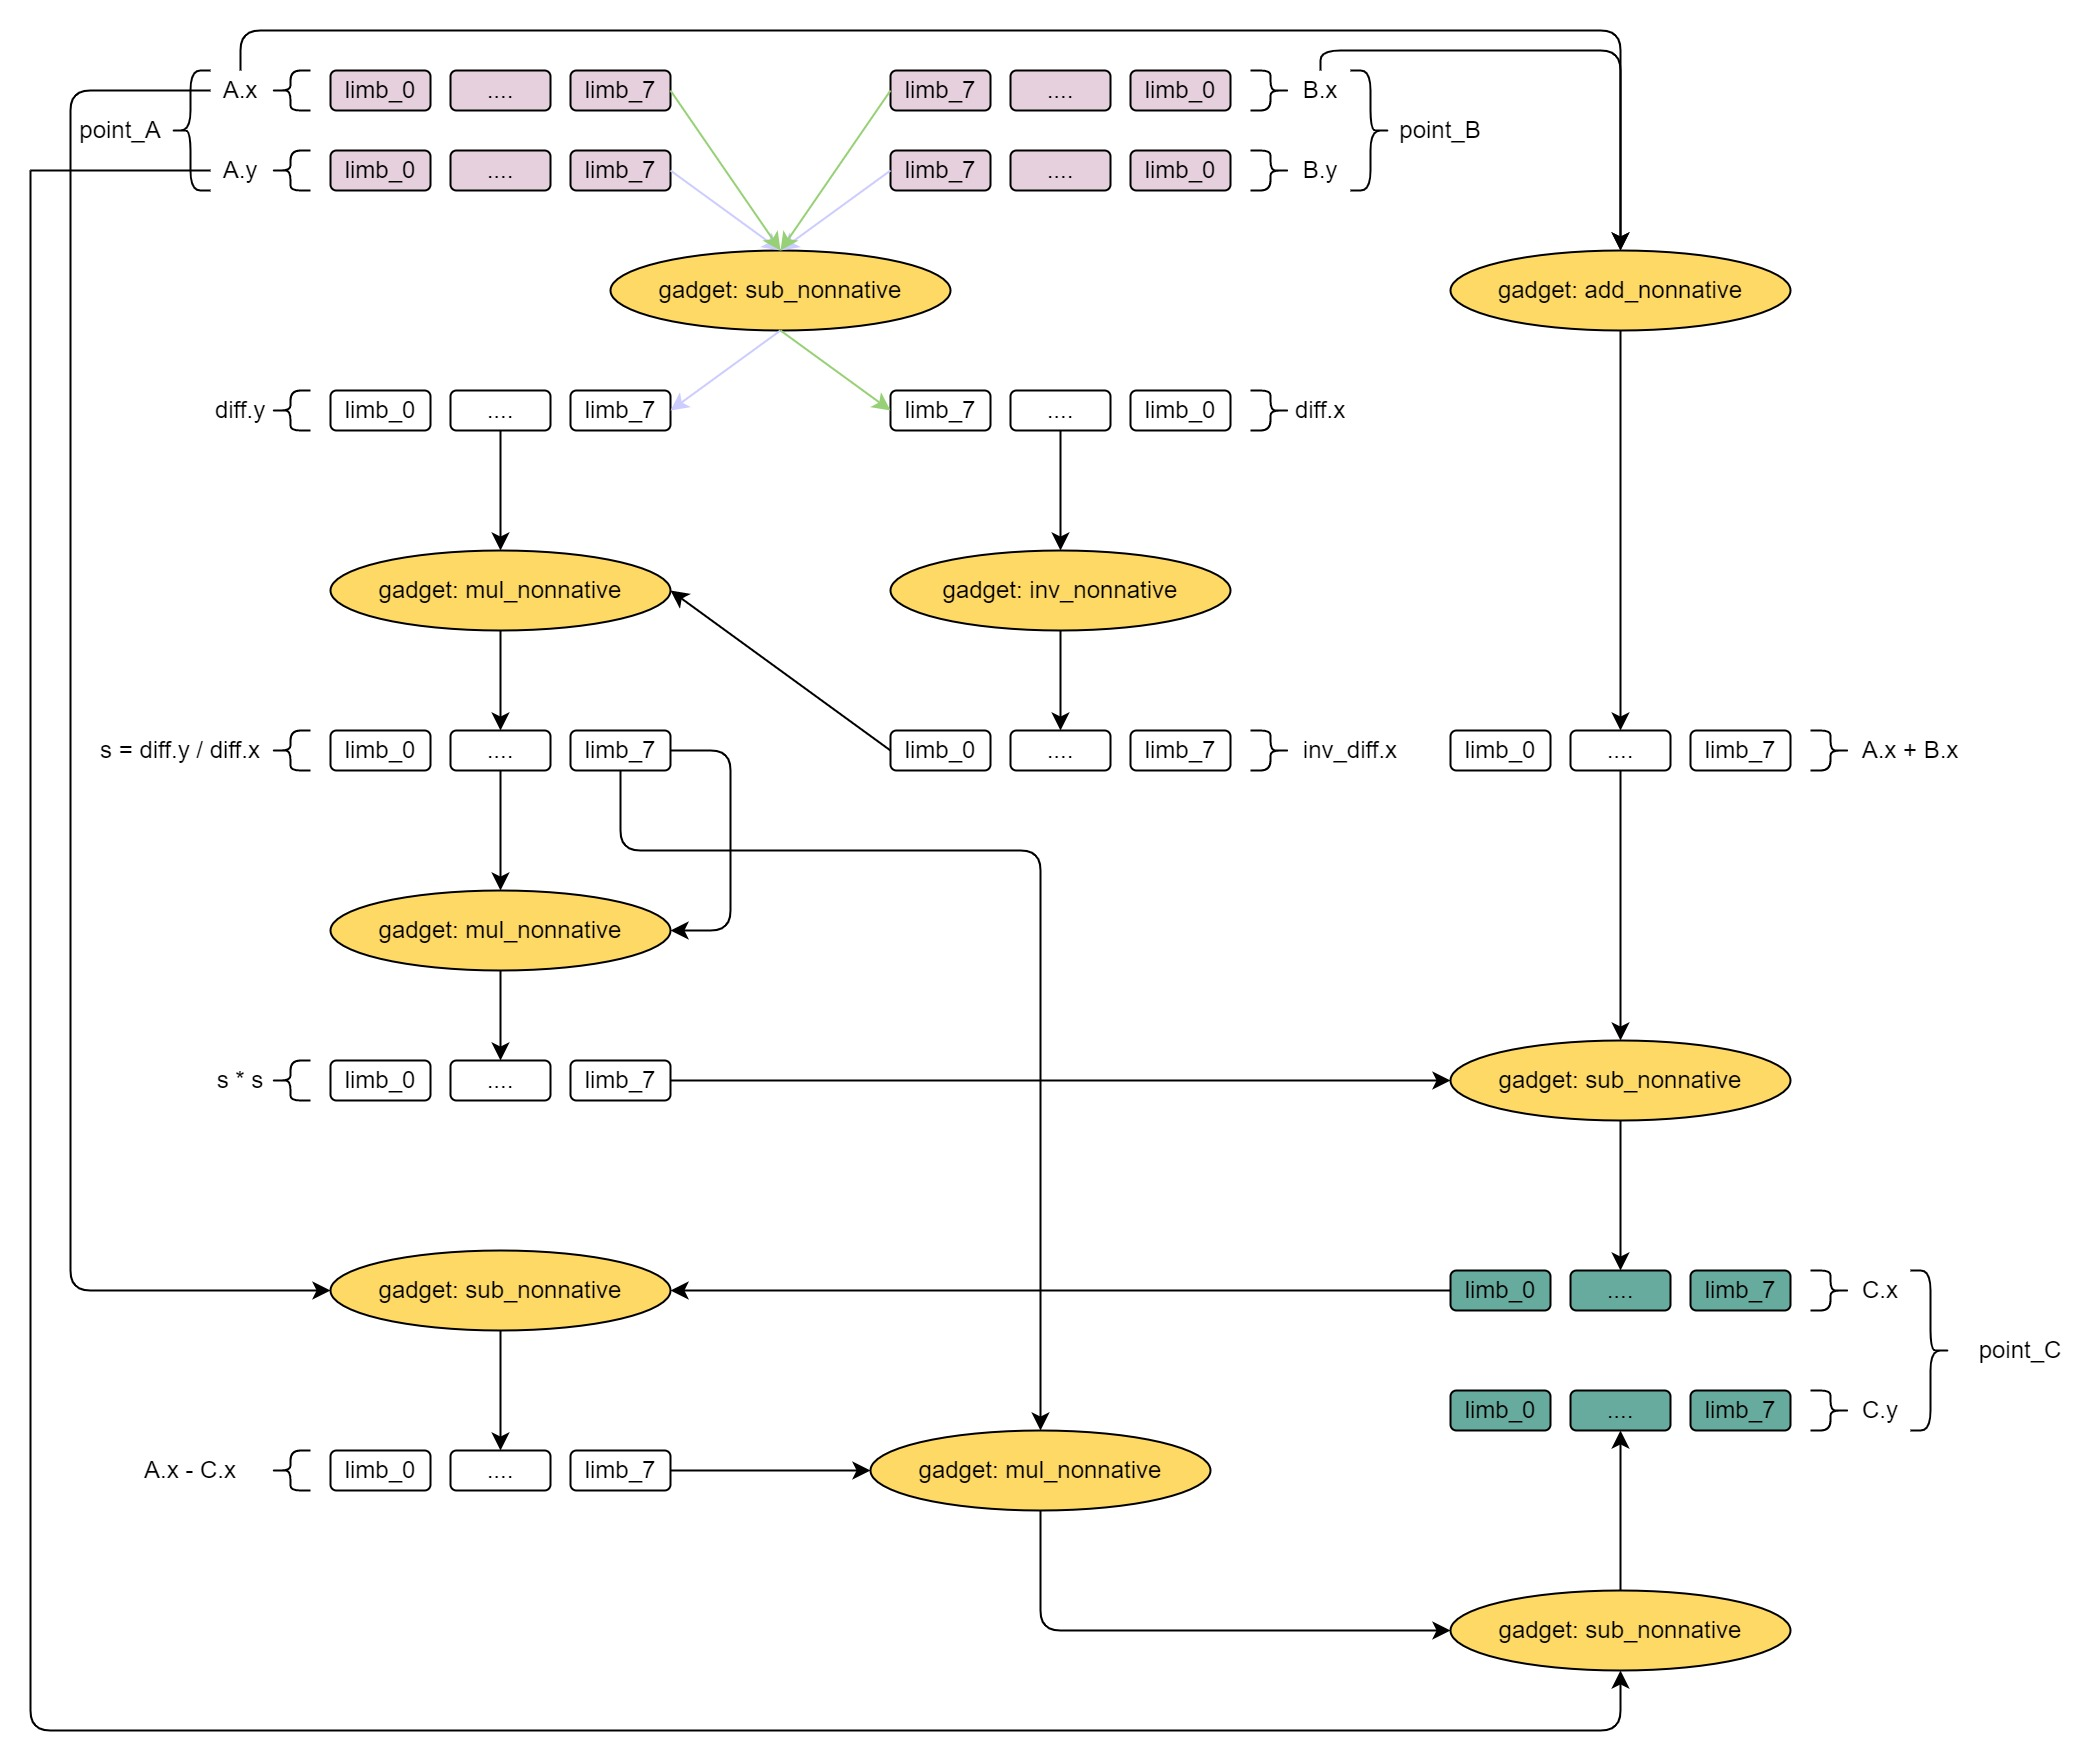
\includegraphics[width=0.6\textwidth]{curve-add-layout.jpg}
    \caption{curve-add layout}
    \label{fig:curve-add-layout}
\end{figure}

\subparagraph{Constraints info and costs}
\begin{itemize}
    \item gadget-sub-nonnative num: 5
    \item gadget-add-nonnative num: 1
    \item gadget-mul-nonnative num: 3
    \item gadget-inv-nonnative num: 1
    \item gate type num: 14
        \begin{itemize}
            \item 8: U32AddManyGate\{2,3,5,7,9,11,13,15\}
            \item 1: ComparisonGate
            \item 1: ArithmeticGate
            \item 1: U32ArithmeticGate
            \item 1: U32SubtractionGate
            \item 2: U32RangeCheckGate\{0,8\}
        \end{itemize}
\end{itemize}

\paragraph{curve-double}

\subparagraph{target}
Implement the addition of two same curve points. this is an incomplete addition, you can refer to The halo2 Book\cite{website:halo2-book} to learn more about it.

\subparagraph{Constraints logic}
$(x_1,y_1) = (x_2,y_2)$. See \figref{fig:curve-add}.

\subparagraph{Process layout}
See \figref{fig:curve-double-layout}.
\begin{figure}[!ht]
    \centering
    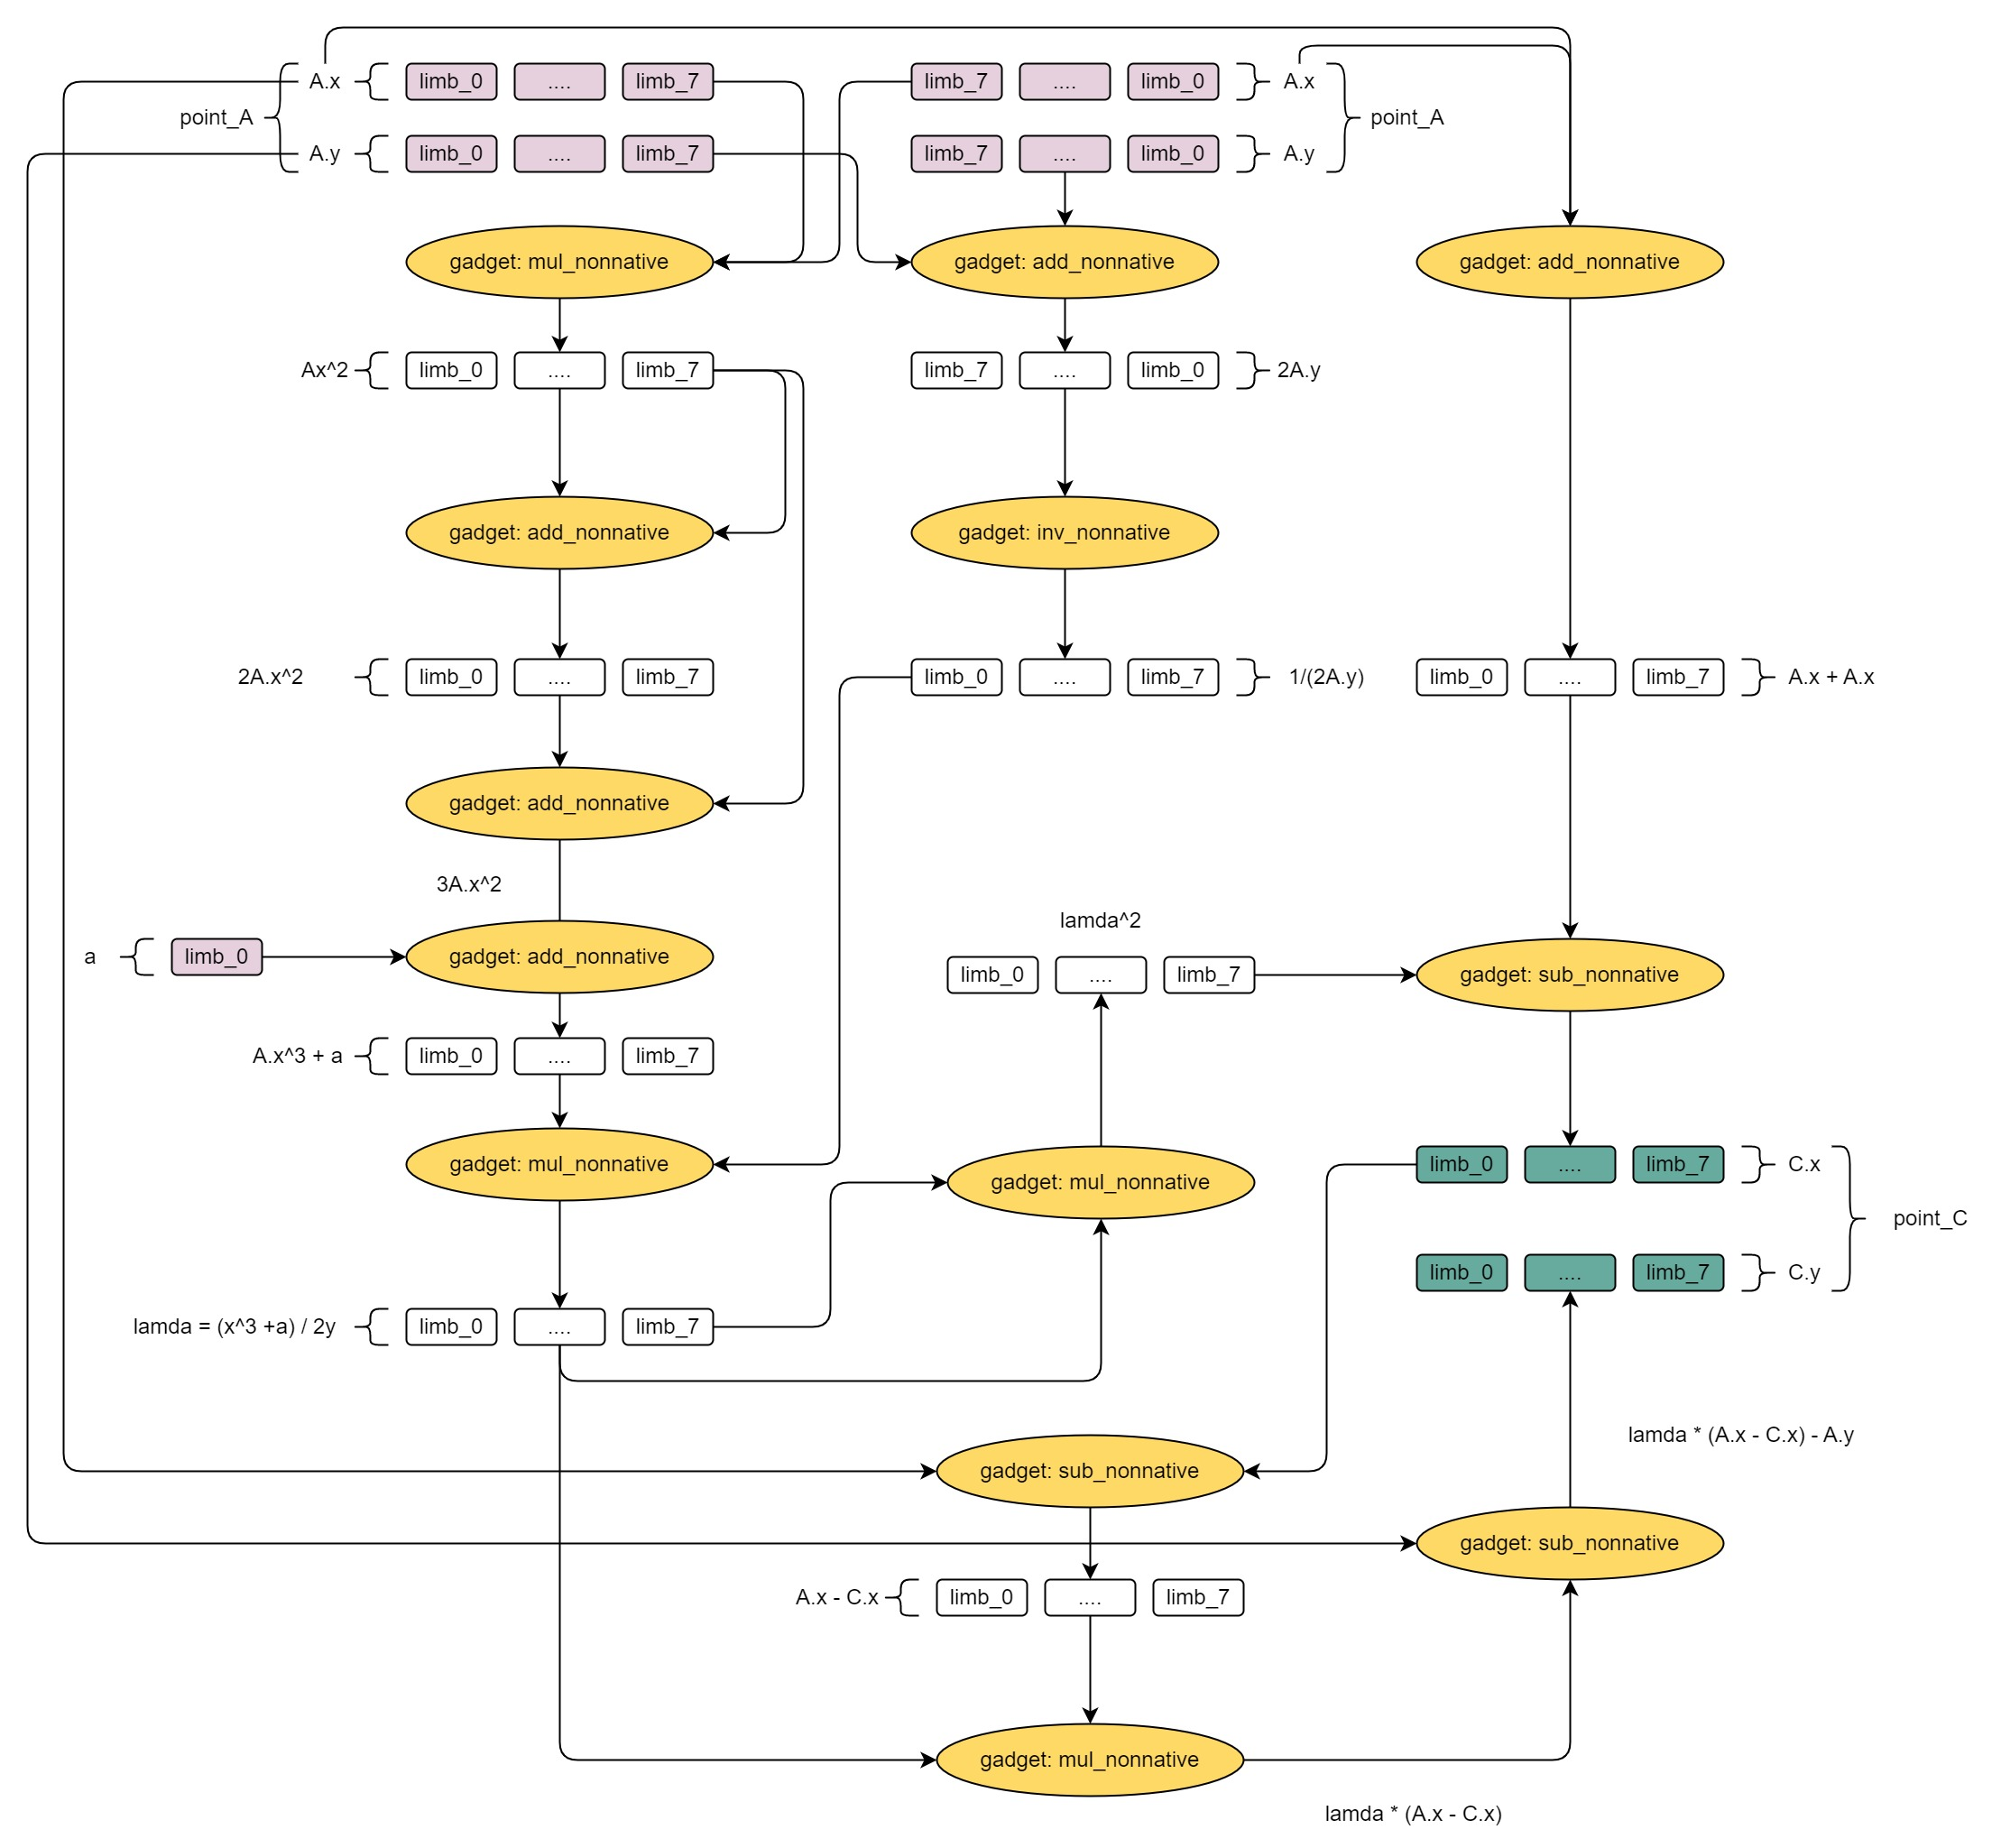
\includegraphics[width=0.6\textwidth]{curve-double-layout.jpg}
    \caption{curve-double layout}
    \label{fig:curve-double-layout}
\end{figure}

\subparagraph{Constraints info and costs}
\begin{itemize}
    \item gadget-sub-nonnative num: 3
    \item gadget-add-nonnative num: 5
    \item gadget-mul-nonnative num: 4
    \item gadget-inv-nonnative num: 1
    \item gate type num: 14
        \begin{itemize}
            \item 8: U32AddManyGate\{2,3,5,7,9,11,13,15\}
            \item 1: ComparisonGate
            \item 1: ArithmeticGate
            \item 1: U32ArithmeticGate
            \item 1: U32SubtractionGate
            \item 2: U32RangeCheckGate\{0,8\}
        \end{itemize}
\end{itemize}

\paragraph{curve-assert-valid}

\subparagraph{Target}
Check point is on the curve $y^2 = x^3 + ax + b$.

\subparagraph{Process layout}
See \figref{fig:curve-assert-valid-layout}.
\begin{figure}[!ht]
    \centering
    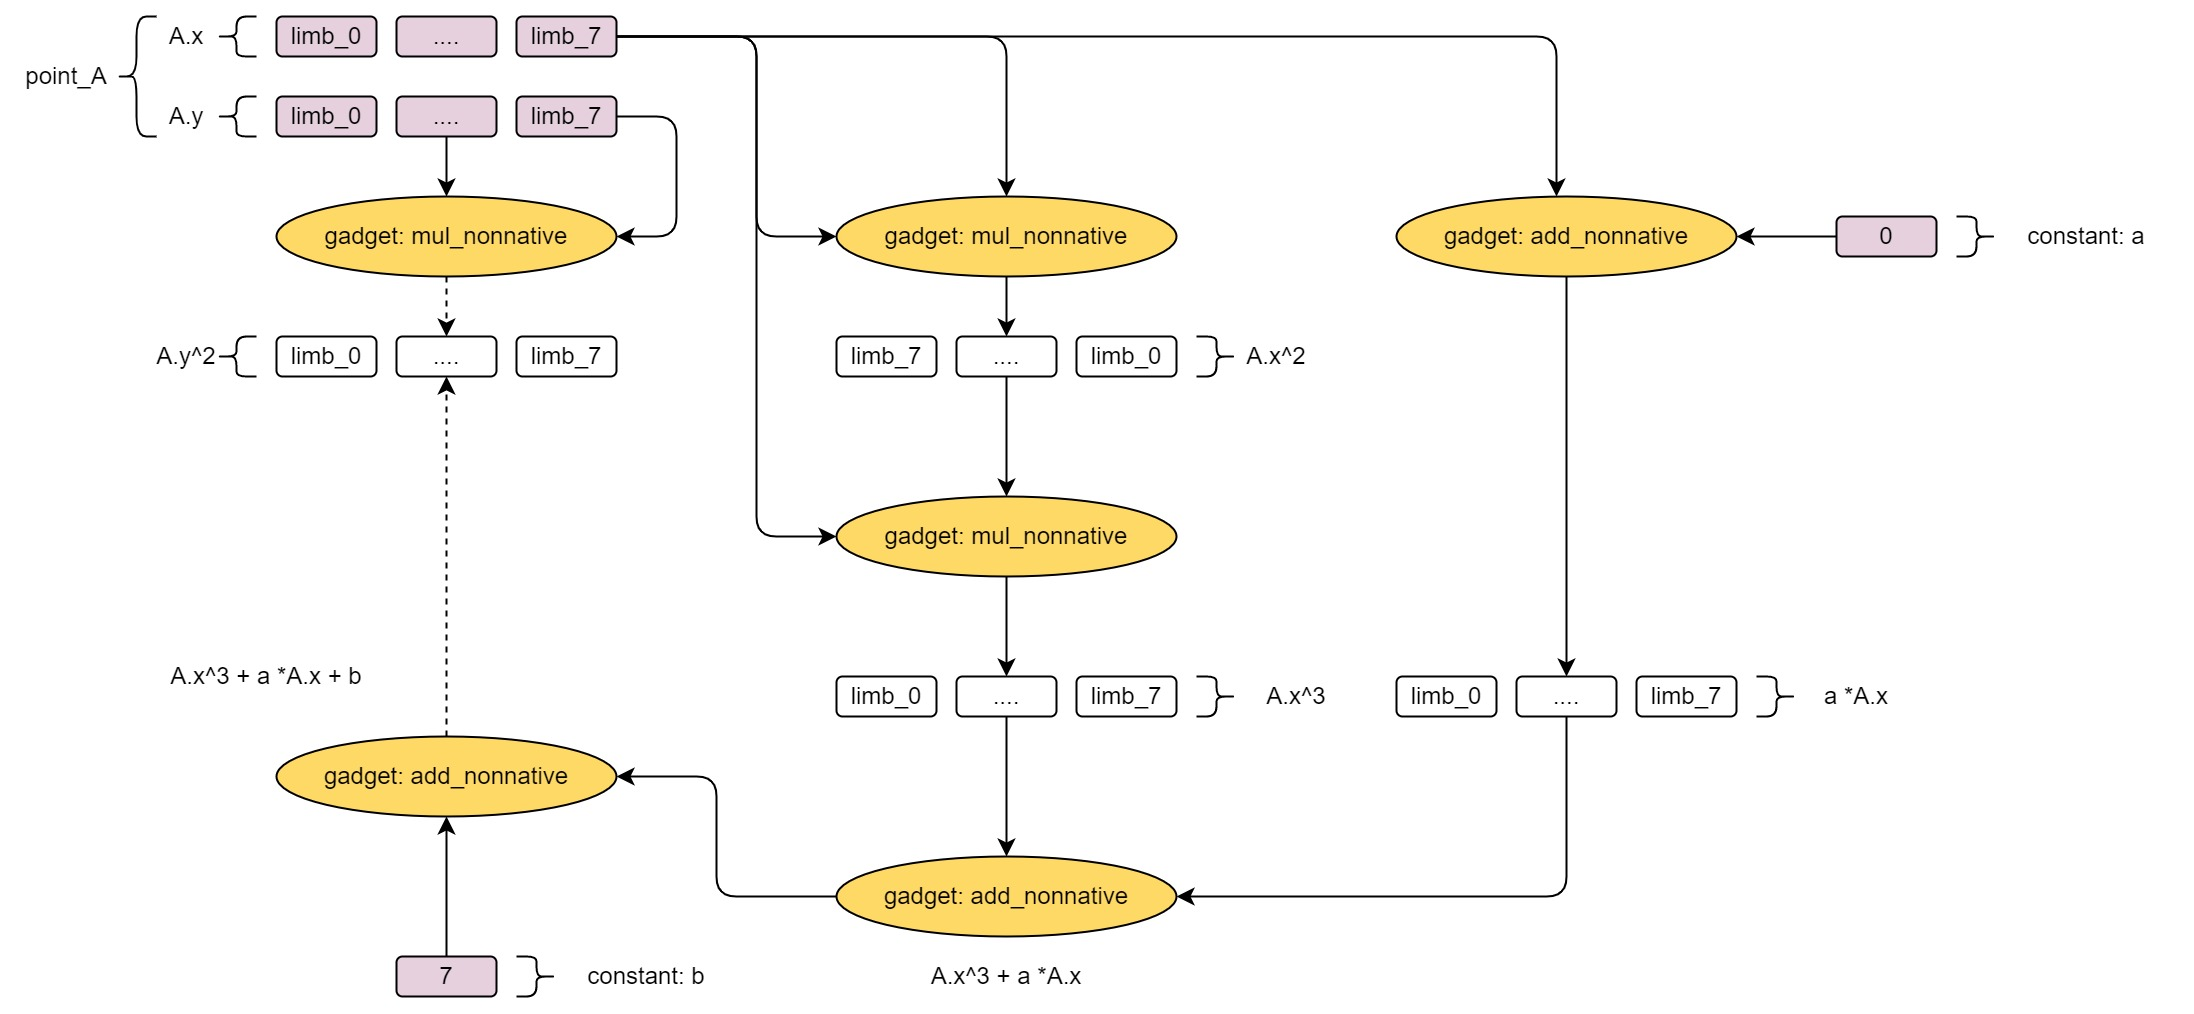
\includegraphics[width=0.5\textwidth]{curve-assert-valid-layout.jpg}
    \caption{curve-assert valid layout}
    \label{fig:curve-assert-valid-layout}
\end{figure}

\subparagraph{Constraints info and costs}
\begin{itemize}
    \item gadget-add-nonnative num: 3
    \item gadget-mul-nonnative num: 3
    \item gate type num: 13
        \begin{itemize}
            \item 8: U32AddManyGate\{2,3,5,7,9,11,13,15\}
            \item 1: ComparisonGate
            \item 1: ArithmeticGate
            \item 1: U32ArithmeticGate
            \item 2: U32RangeCheckGate\{0,8\}
        \end{itemize}
\end{itemize}
  
\paragraph{curve-msm}

\subparagraph{target}
Implement the multiplication scalar multiplication (MSM).

\subparagraph{Constraints logic}
See \figref{fig:curve-msm}.
\begin{figure}[!ht]
    \centering
    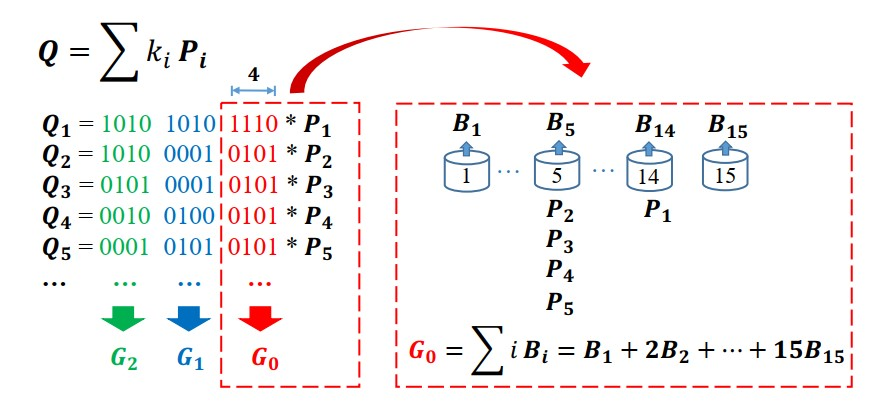
\includegraphics[width=0.5\textwidth]{curve-msm.jpg}
    \caption{curve-msm}
    \label{fig:curve-msm}
\end{figure}

\subparagraph{Constraints info and costs}
\begin{itemize}
    \item gate type num: 14
    \item gate instance num: 147553
\end{itemize}

\subsubsubsection{curve-scalar}

\begin{enumerate}
    \item \verb|Target|: Implement the multiplication between scalar and point.
    \item \verb|Constraints logic|: See \figref{fig:curve-scalar}.
    \item \verb|Constraints info and costs|:
    \begin{itemize}
        \item gate type num: 13 
        \item gate instance num: 180364          
    \end{itemize}
\end{enumerate}

\begin{figure}[!ht]
    \centering
    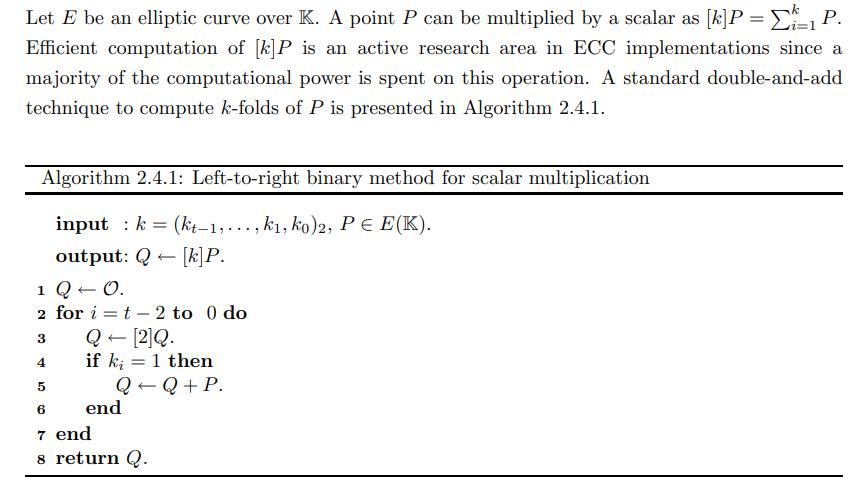
\includegraphics[width=0.6\textwidth]{curve-scalar.jpg}
    \caption{curve-scalar}
    \label{fig:curve-scalar}
\end{figure}


\paragraph{ecdsa}

\subparagraph{Target}
Implement ecdsa verify process.

\subparagraph{Constraints logic}
\begin{figure}[!ht]
    \centering
    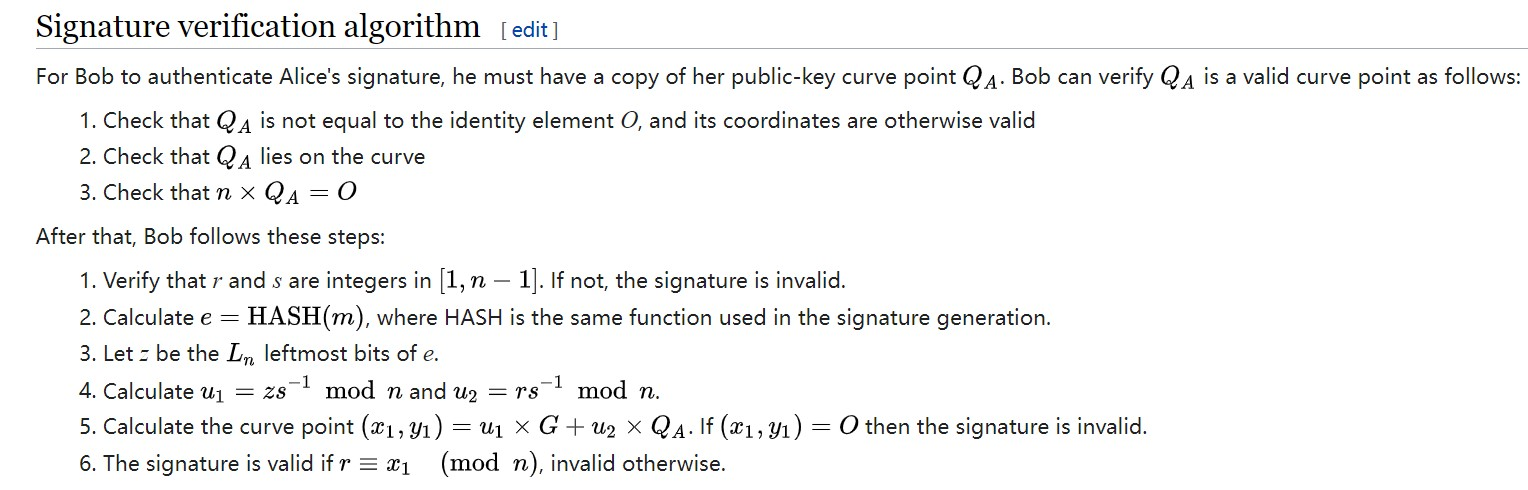
\includegraphics[width=0.5\textwidth]{ecdsa.jpg}
    \caption{ecdsa}
    \label{fig:ecdsa}
\end{figure}

\subparagraph{Constraints info and costs}
\begin{itemize}
    \item gate type num: 16
    \item gate instance num: 98039
\end{itemize}



\subsection{Inner Table Lookup}\label{section: inner-table-lookup}

Inner-table lookup can be thought of as a subset argument technology between columns I and T, proving that cells in column I all appear in column T at least once, and it does not matter whether the cells in column T are in I. To simplify the calculation, the columns in the STARK table are all $2^k$ rows, and when the cells of columns I and T are not $2^k$, they need to be extended.

\begin{itemize}
    \item Cells in column I can be extended with elements in column I or column T
    \item Cells in column T can only be extended with cells in column T, usually the last one
\end{itemize}

The inner-table lookup technology is to first generate the corresponding permutation columns I' and T' from columns I and T, respectively. The permutation relationship between I and I', T and T' can be checked through the permutation argument during the proving phase:
$$Z(\omega X) \cdot (I'(X) + \beta) \cdot (T'(X) + \gamma) - Z(X) \cdot (I(X) + \beta) \cdot (T(X) + \gamma) = 0$$
$$1 - Z(\omega^0) = 1 - Z(\omega^{k}) = 0$$

\noindent Then sort columns I' and T' as follows:

\begin{enumerate}
    \item Column I' is ordered by a sorting algorithm so that cells of the same value are adjacent to each other.
    \item Column T' is ordered so that the first row in a sequence of the same values in I' has the same value in T' at the same position.
\end{enumerate}

\noindent Now, we'll enforce either $I'_{i} = T'_{i}$ or that $I'_{i}=I'_{i-1}$, using the rule:
$$(I'(X) - T'(X)) \cdot (I'(\omega X) - I'(X)) = 0$$
$$I'(\omega^0) - T'(\omega^0) = 0$$

These constraints effectively force every element in I' (and thus I) to equal at least one element in T' (and thus T).
\subsection{Cross Table Lookup}\label{section: cross-table-lookup}

The goal of cross table lookup is different from that of inner-table lookup, which is not only a subset argument, but a mix of subset argument and permutation argument.

Cross table lookup indicates the multi-table lookup in the plookup \cite{cryptoeprint:2020/315,}, that is, the data in a looked table comes from multiple looking tables. When implementing STARK tables, Starky should define all the STARK cross table lookup relationships, that is, which other STARK tables each STARK table needs to look from, and which columns and rows are involved(filtered) in the looked table and looking table respectively during the lookup. Each STARK table needs to perform cross table lookups, so there are multiple CrossTableLookups in Starky, and each cross table lookup instance consists of a looked table and multiple looking tables.

We generate a Z(X) polynomial from calculating the permutation product as the grand product argument polynomial for the permutation argument in a cross table lookup instance, and then enforce that they are permutations using a permutation argument with Z(X) polynomial

\begin{enumerate}
    \item Initialize cross table lookup instances and random numbers $\beta, \gamma$
    \item Calculate the partial products of the looking table and looked table, compressing the values of multiple columns into one:$$C = \Pi(c_i * \beta^i) + \gamma$$
    \item Calculate Z(X) polynomial from partial products $$Z(\omega X) = Z(X)\cdot (C \cdot filter + 1 - filter)$$
    \item Verify that the product of the last element of the Z(X) polynomials of all looking tables is equal to the last element of the Z(X) of the looked table
    $$\Pi_{i=0} Z^{looking}_{i}(\omega^{k_i-1}) = Z^{looked}(\omega^{k_{looked}-1})$$
\end{enumerate}

Cross table lookup enforces STARK tables are correctly generated from the program, and reduces the rows in CPU STARK table.

\subsection{GPU Acceleration}\label{section: gpu-acceleration}
The polynomial computations of ZK mainly consists of multiple NTTs and INTTs. In our ZK framework, the maximum size of NTTs is $2^{23}$. The large-size NTTs result in sigificant challenges for both off-chip memory accesses and on-chip compute resources, due to the irregular strided access patterns similar to classical FFTs. The GPU acceleration section takes full advantage of GPU multi-threaded parallel processing to speed up NTT calculations.
\subsubsection{NTT Computations}
The NTT computation is defined as
\[\hat{a} = NTT{(a)}\]
Where $a$ and  $\hat{a}$ are two $N$ size arrays, and  $\hat{a}[i] = \sum_{j=0}^{N-1} a[j] \omega_N^{ij}$. Here $a[i]$ and $\hat{a}[i]$ are $\lambda$-bit scalars in a finite field. And $\omega_N$is the $N$-th root of unity in the same field, also is called twiddle factor, which is a constant value for a specific size of $N$.

Similar to classical FFTs, optimized and improved performance implementations of the NTT are of necessity and fundamental essentials. Cooley-Tukey processing is a commonly used NTT algorithm in science and engineering. For example, the Cooly-Tukey algorithm reduces the computational complexity from $O(N^2)$ to $O(NlogN)$. Its fundamental idea is to recursively decompose a large-size NTT into several linear combinations of smaller NTTs. The butterfly network of Cooley-Tukey NTT is a decimation-in-time network whereby its twiddle factor appears on the input side of calculation and input data are arranged in bit-reversed order. Fig.1 illustrates the butterfly networks of Cooley-Tukey NTT. The NTT optimization mainly involves butterfly network and butterfly computing.
\subsubsection{2-D NTT}
NTT is an important kernel commonly used in our ZK scheme. In fact, there exist many accelerator designs for NTT. However, the polynomial computations in our ZK scheme have substantially larger scales than those addressed in other ZK. It requires multiple NTTs of up to $2^{23}$ elements, Such large sizes can hardly be satisfied by any previous GPU design.

To overcome the large-sizes challenges, we adopt a 2-D NTT algorithm to decompose a large NTT into multiple smaller NTT kernels (4096/8192). This allows GPU to only implement smaller NTT modules, which can fit into the compute resources (e.g. the stream processor number of on GPU). Then the original large-size NTT can be calculated by iteratively using the smaller NTT.

The overview of 2-D NTT algorithm is shown in Figure 2. First of all, a large NTT size N is decomposed into P rows and Q columns, with N=P×Q. Then the N-size NTT can be calculated by several P-size and Q-size smaller NTTs. Firstly, the P-size NTT is parallel computing using the same twiddle factors for each of the Q columns. The output is still a P-size vector. Before the second dimensional NTT, a corresponding twiddle factor $\omega^{ij}$ is multiplied to each element of the output vector. Finally, a Q-size NTT for each of the P rows is parallel computing. The output column-major order elements is the result of the large-size NTT.
\subsubsection{GPU and CUDA}
Currently, the GPU is no longer limited to graphics processing. Thanks to the rapid evolution of their architecture that made it straightforward to access their underlying powerful Parallelism to address different categories of data parallel algorithms to be handled efficiently by this platform. The GPU is designed to process a huge amount of numbers operations in parallel relying on thousands of computing cores running concurrently. CUDA is a general-purpose parallel computing architecture that delivers a novel parallel programming paradigm and a new instruction set architecture that can easily leverage the parallel power of the computing engine embedded in the CUDA-enabled GPUs to solve complex scientific and engineering applications. It becomes straightforward to decompose the computations into fine-grained threads and execute theses threads on the device in parallel. CUDA refers to the software platform and the hardware architecture used to execute the kernels. A kernel launches thousands of threads for parallel execution organized in three levels: grids, blocks, and warps. The grids are two- or three-dimensional arrangements of threads blocks where every block consists of an upper limit of threads 512 or 1024 depending on the compute capability version of the device, and finally each group of threads form a wrap. Such architecture is called Single Instruction Multiple Thread (SIMT); which allows the GPU to execute single instruction on multiple concurrent threads operating on different data. Every running thread has access to some built-in variable assigned by the CUDA run time system and used for thread indexing. CUDA also has an efficient memory hierarchy divided in global, shared, register, texture, and constant memory.
\subsubsection{Implement of 2-D NTT with GPU}
To overcome the large-sizes challenges on GPU, the 2-D NTT algorithm is adopted. For a particular GPU model, the number of stream processors has been set to a fixed value, so the total number of threads running simultaneously on this GPU is limited. In order to make full use of the GPU thread resources, we set NTT's two-dimensional running framework as shown below. The NTT sequence is divided into 8192 rows and 1024 columns. For each column, 8192 threads (This number can be adjusted based on the number of stream processors to achieve maximum GPU utilization) are allocated to calculate 8192-size 1D NTT in parallel.

After processing each column, the NTT of the second dimension can process 8 rows at a time through the Cooperative Groups (CG) mechanism. The Cooperative Groups programming model describes synchronization patterns both within and across CUDA thread blocks. It provides CUDA device code APIs for defining, partitioning, and synchronizing groups of threads. It also provides host-side APIs to launch grids whose threads are all guaranteed to be executing concurrently to enable synchronization across thread blocks. These primitives enable new patterns of cooperative parallelism within CUDA, including producer-consumer parallelism and global synchronization across the entire thread grid or even multiple GPUs.

Therefore, the total running time of the GPU is 1024 8192-size NTTs plus 1024 1024-size NTTs.
\subsubsection{Memory Access}
The following figure shows the CUDA memory model. The large-size NTT data is copied from the host into global memory. Then it is sent to shared memory into the compute queue. For faster access, precomputed twiddle factors are stored in texture memory. When the twiddle factor is used, it is copied sequentially to the registers according to the index. The results of one-dimensional NTTs are saved in shared memory. When the NTT is calculated, the output is copied from shared memory to global memory and uploaded to the host.

\subsection{FPGA Acceleration}\label{section: fpga-acceleration}

The NTT acceleration design consists of two main parts: the NTT engine and the DMA data transfer engine. The NTT engine performs calculations on given-length data points, while the DMA data transfer engine efficiently exchanges data between the NTT engine and DDR.

\begin{figure}[ht]
  \centering
  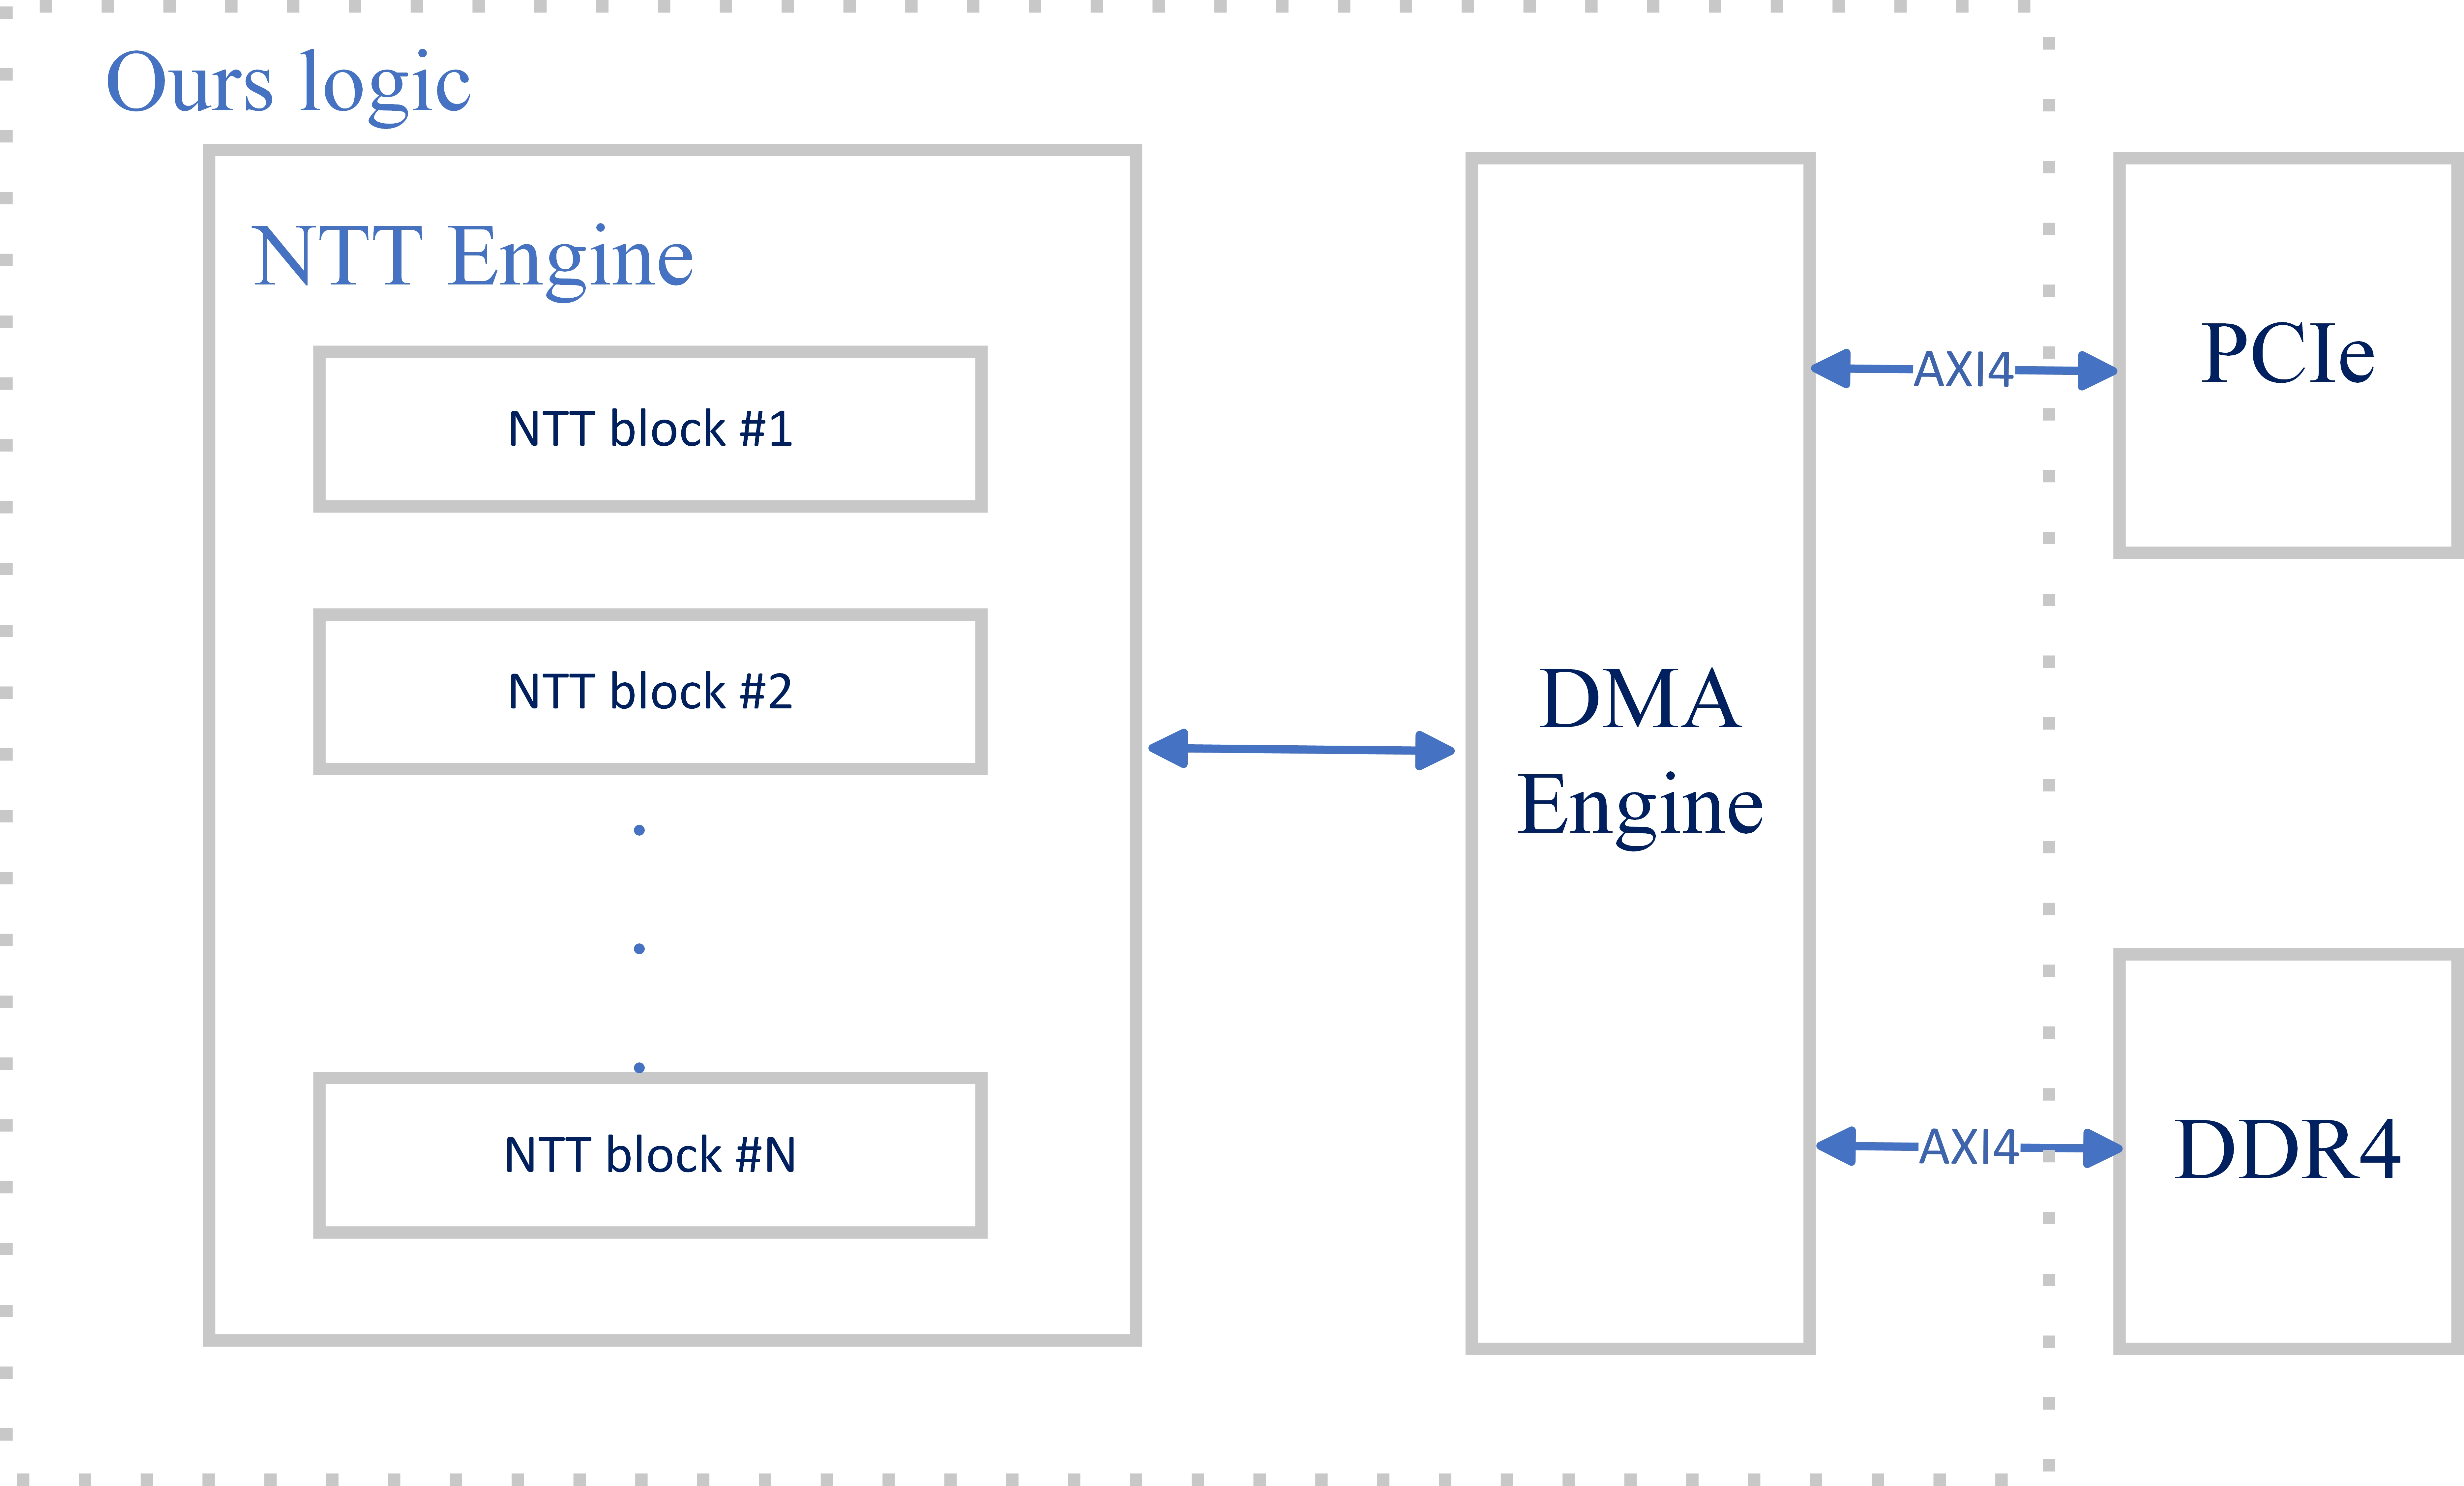
\includegraphics[width=0.8\textwidth]{The design of NTT acceleration implemented in FPGA.jpg}
  \caption{The design of NTT acceleration implemented in FPGA}
  \label{fig:The design of NTT acceleration implemented in FPGA}
\end{figure}

\subsubsection{NTT engine}

In this design, the NTT engine consists of multiple parallel-running NTT modules. The maximum supported data length for a single NTT module is $2^{12}$. Moreover, a  modular multiplication unit is connected to the output of each NTT module to support the extension of two-dimensional or higher-dimensional NTTs. To improve scalability performance, variable-length NTT calculations can be achieved through parameter configuration through the AXI4 interface.

In practical applications, processing in parallel with multiple NTT modules can greatly improve computational performance. For a single NTT module, one point reading and one storage operation are required per clock cycle. When 8 NTTs are processed in parallel in the engine, the total access bandwidth required is 8 * 8 byte/point * (1x read + 1x write) * 100MHz = 11.92 GB/sec with assuming a working clock of 100MHz. That is, the calculation rate of NTT is 8 * 100MHz / $2^{24}$ / 2= 25 times/sec. For the AWS FPGA platform, the user logic can use three DDR4 channels with a interface frequency up to 2100MHz. The total supported simultaneous access bandwidth is 3 * 8 byte/DDR * 2100MHz = 46.9 GB/sec. Therefore, the maximum supported NTT calculation rate is 25 * 46.9 / 11.92 = 98 times/sec.


\paragraph{NTT calculation module}

To support NTT calculation with the length of $2^{24}$, it is better to consider the $2^{24}$ points as a 2D array with a size of $2^{12}$ points by $2^{12}$ points. Using the Gentleman-Sande algorithm, the first pass through the engine computes $2^{12}$ NTTs column-wise of the 2D array using the carefully designed NTT module with a length of $2^{12}$. For this module, a recursive NTT Algorithm is adopted, which contains 12 stages of butterfly with varying kernel sizes. Users can adjust the sizes of both columns and rows in the 2D array by setting parameters to meet FPGA running requirements. Finally, the output of the NTT block performs modular multiplication according to the 2D NTT algorithm.

\begin{figure}[ht]
  \centering
  
\includegraphics[width=1\textwidth]{Various-size NTT block.jpg}
  \caption{Various-size NTT block (MM: modular multiplication)}
  \label{fig:NTT_module}
\end{figure}

\paragraph{NTT kernel}
The NTT block contains several kernels, each of which is mainly composed of a butterfly unit and two RAMs. The butterfly unit is carefully designed to take maximum advantage of the FPGA DSPs, especially by utilizing the tricks of the Goldilocks field multiply to improve computational efficiency over modular reduction. One of the RAMs is used to buffer the input data, while the other stores the twiddle factors required for butterfly calculation.


\begin{figure}[ht]
  \centering
  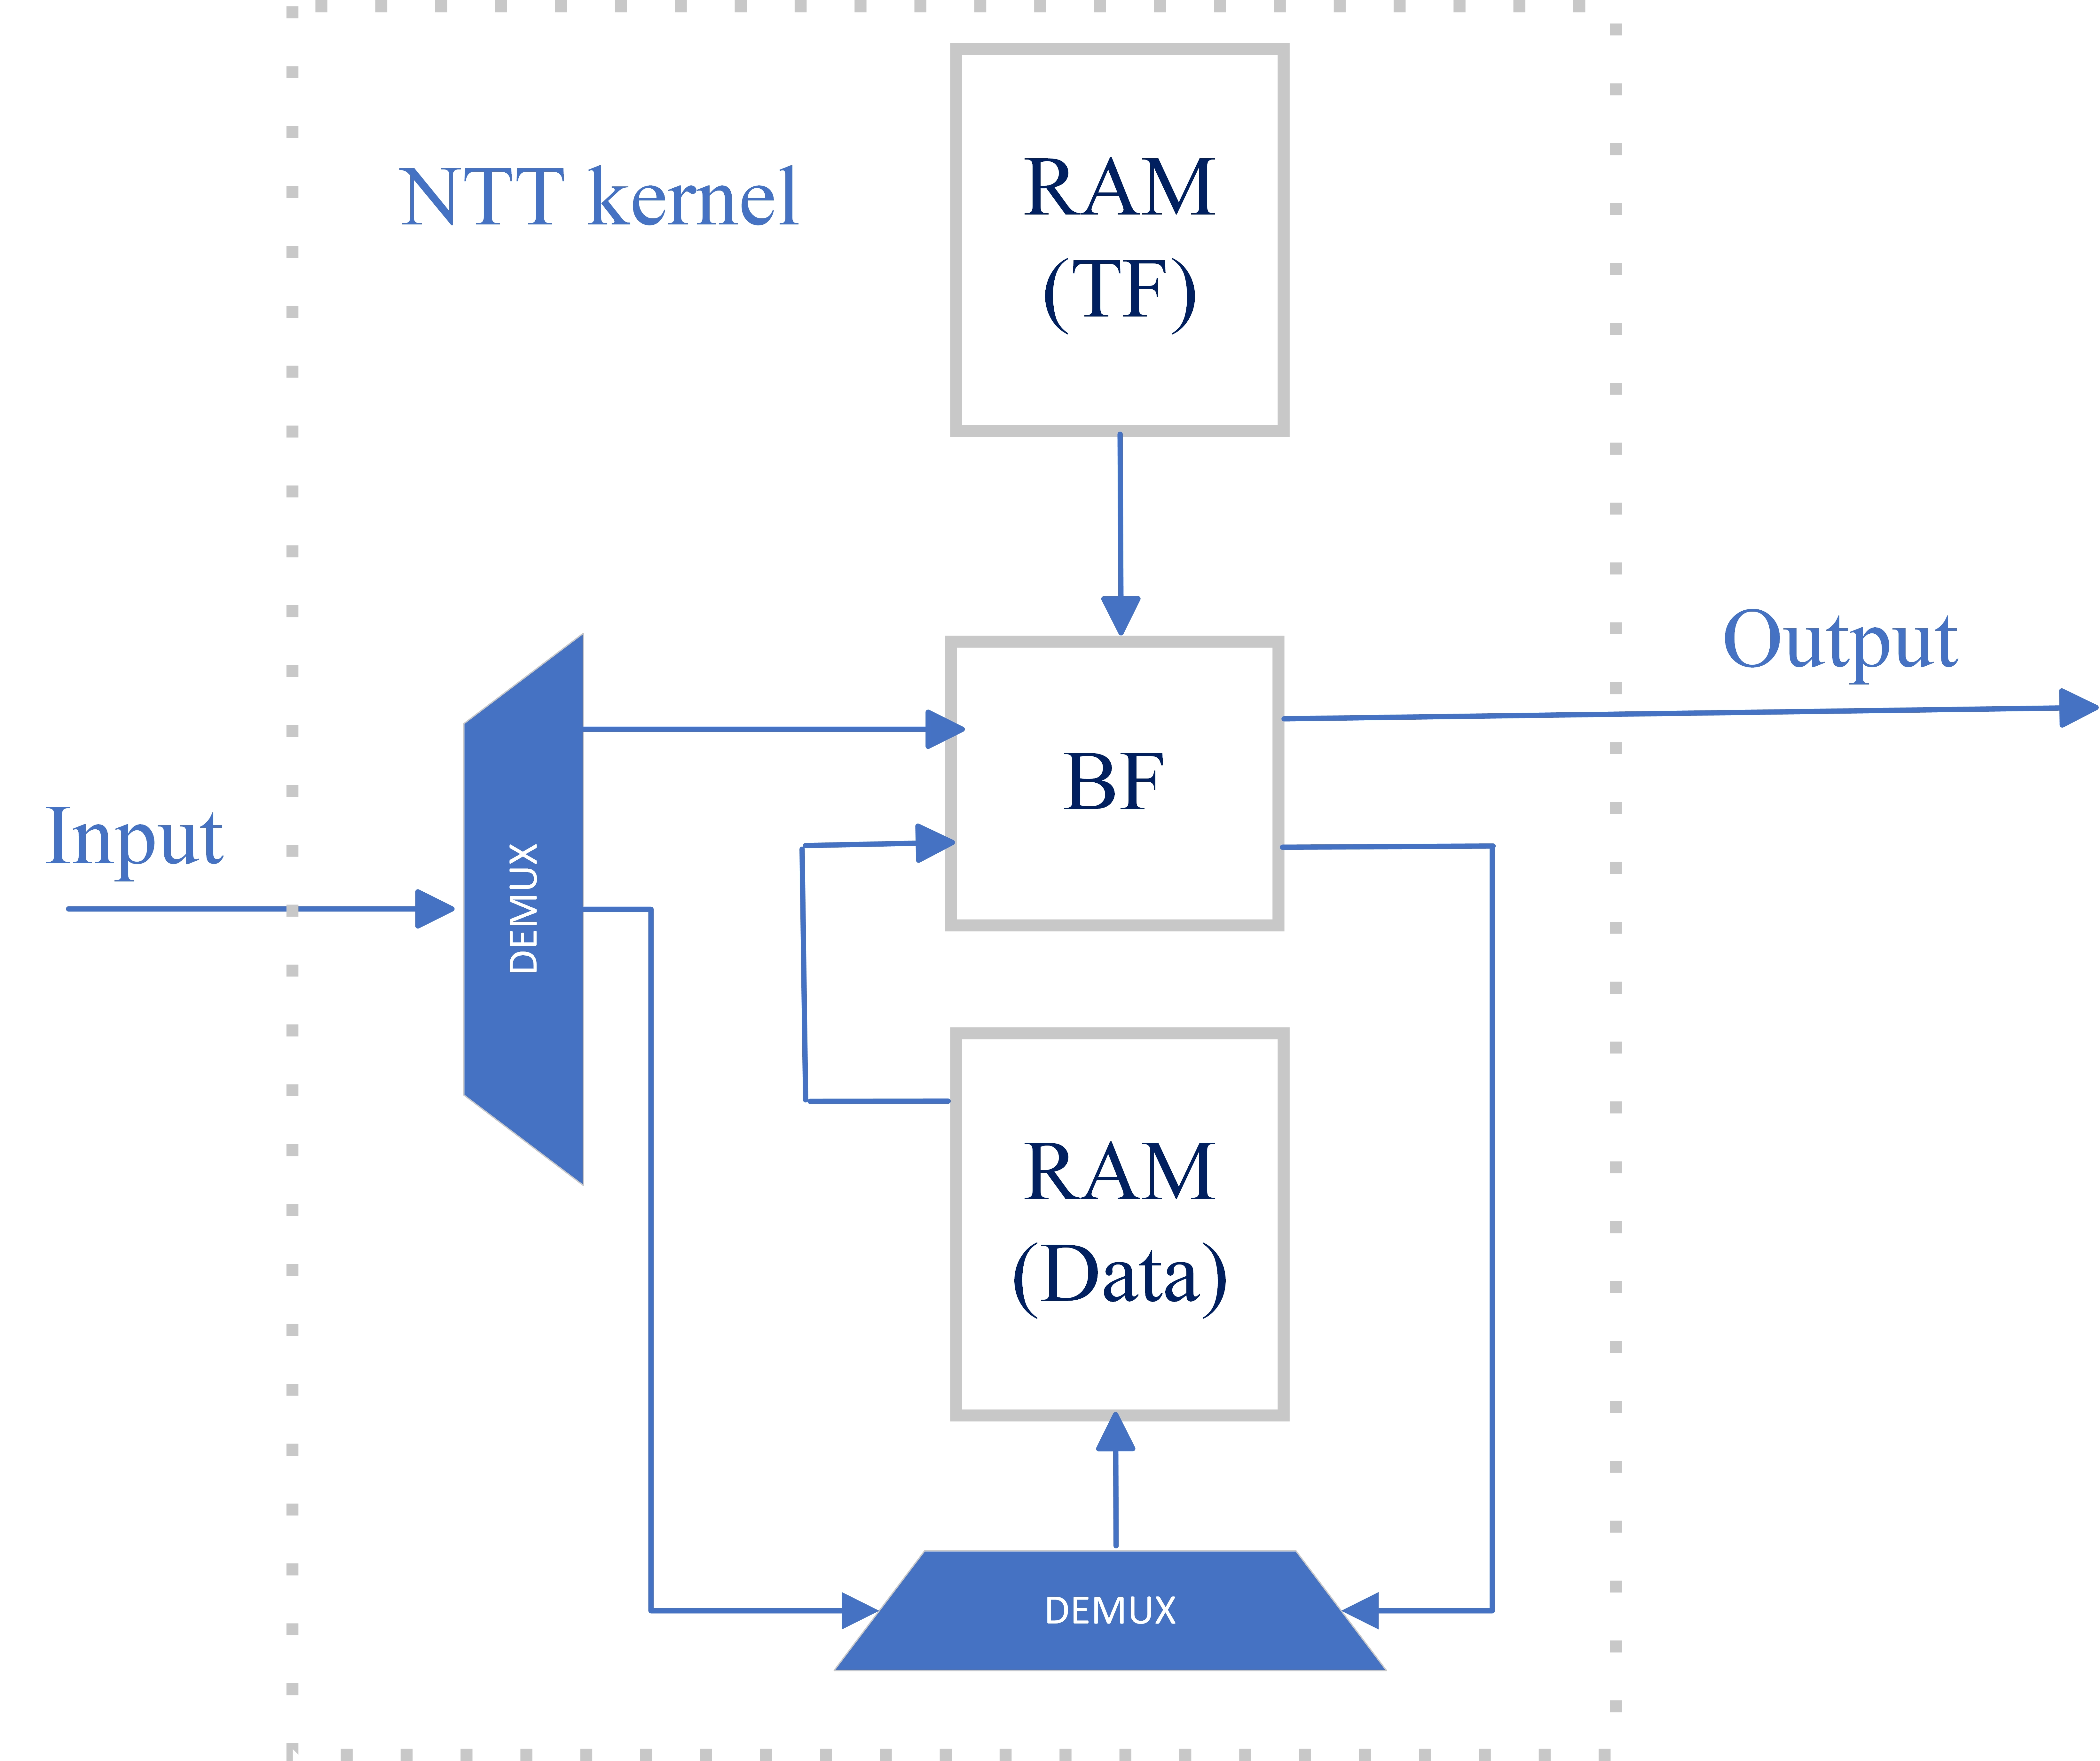
\includegraphics[width=0.5\textwidth]{NTT kernel.jpg}
  \caption{NTT kernel (TF: twiddle factor; BF: Butterfly)}
  \label{fig:NTT_kernel}
\end{figure}

\paragraph{Generation of twiddle factors}

To realize the 2D NTT, the outputs of the 1st pass with the NTT engine should be multiplied by the corresponding twiddle factors, as shown in Fig.2. Since the twiddle factors required for the NTT output of different columns of the 2D array are different, these twiddle factors must be updated for every column. To reduce the necessary DDR bandwidth, a combination of LUT and computation is used to generate these twiddle factors. The LUT provides  $2^{12}$ twiddles needed for modular multiplication before the 2nd pass.Then, the updating twiddle factor is computed by multiplying the LUT twiddles with an accumulated running twiddle factor and then writing back to the LUTs at the same of modular multiplying. Additionally, the twiddle factors needed in the NTT block are provided by LUTs and loaded once before performing the NTT. Therefore, the total number of multiplication/reduction units per block is 13: 11 for the 12 butterfly stages and 2 for each twiddle updating and modulation multiplication out of the NTT block.

\paragraph{Bit Reversal}
The NTT engine performs bit reversal during NTT computation, which is achieved by bit reversing each pass of the NTT at the end of the block (as shown in the above NTT blocks). A final step is required to complete the bit reversal across the two passes. This can be achieved by writing back the results of the 2nd pass using the column-major access pattern instead of the row-major access pattern.


\subsubsection{DMA Engine}

The sole responsibility of the DMA Engine is to exchange points between the NTT Engine and the memory outside of the FPGA at the NTT Engine's burst processing rate. With the NTT Engine capable of consuming and producing 8 points per cycle when 8 NTT blocks are working concurrently, and an NTT Engine clock rate nearing 300MHz, the feed and sink rates are both 17.9 GB/sec. The FPGA's DDR4 memory, with a peak bandwidth of 46.9 GB/sec, can support the combined feed and sink bandwidth need of 35.8 GB/sec while also providing enough storage for $2^{24}$ points.
  In addition, to fully utilize the bandwidth of DDR4 and continuously provide high data bandwidth to the NTT engine, a large data buffer RAM is introduced in the DMA engine to maintain a high data throughput rate for the AXI4 interface.

\subsubsection{Simulation}

To verify the feasibility of the designed NTT acceleration scheme, it was implemented in Vivado using Verilog HDL language and both functional and timing simulations were performed. The simulation results are shown in the following figure.

\begin{figure}[h]
  \centering
  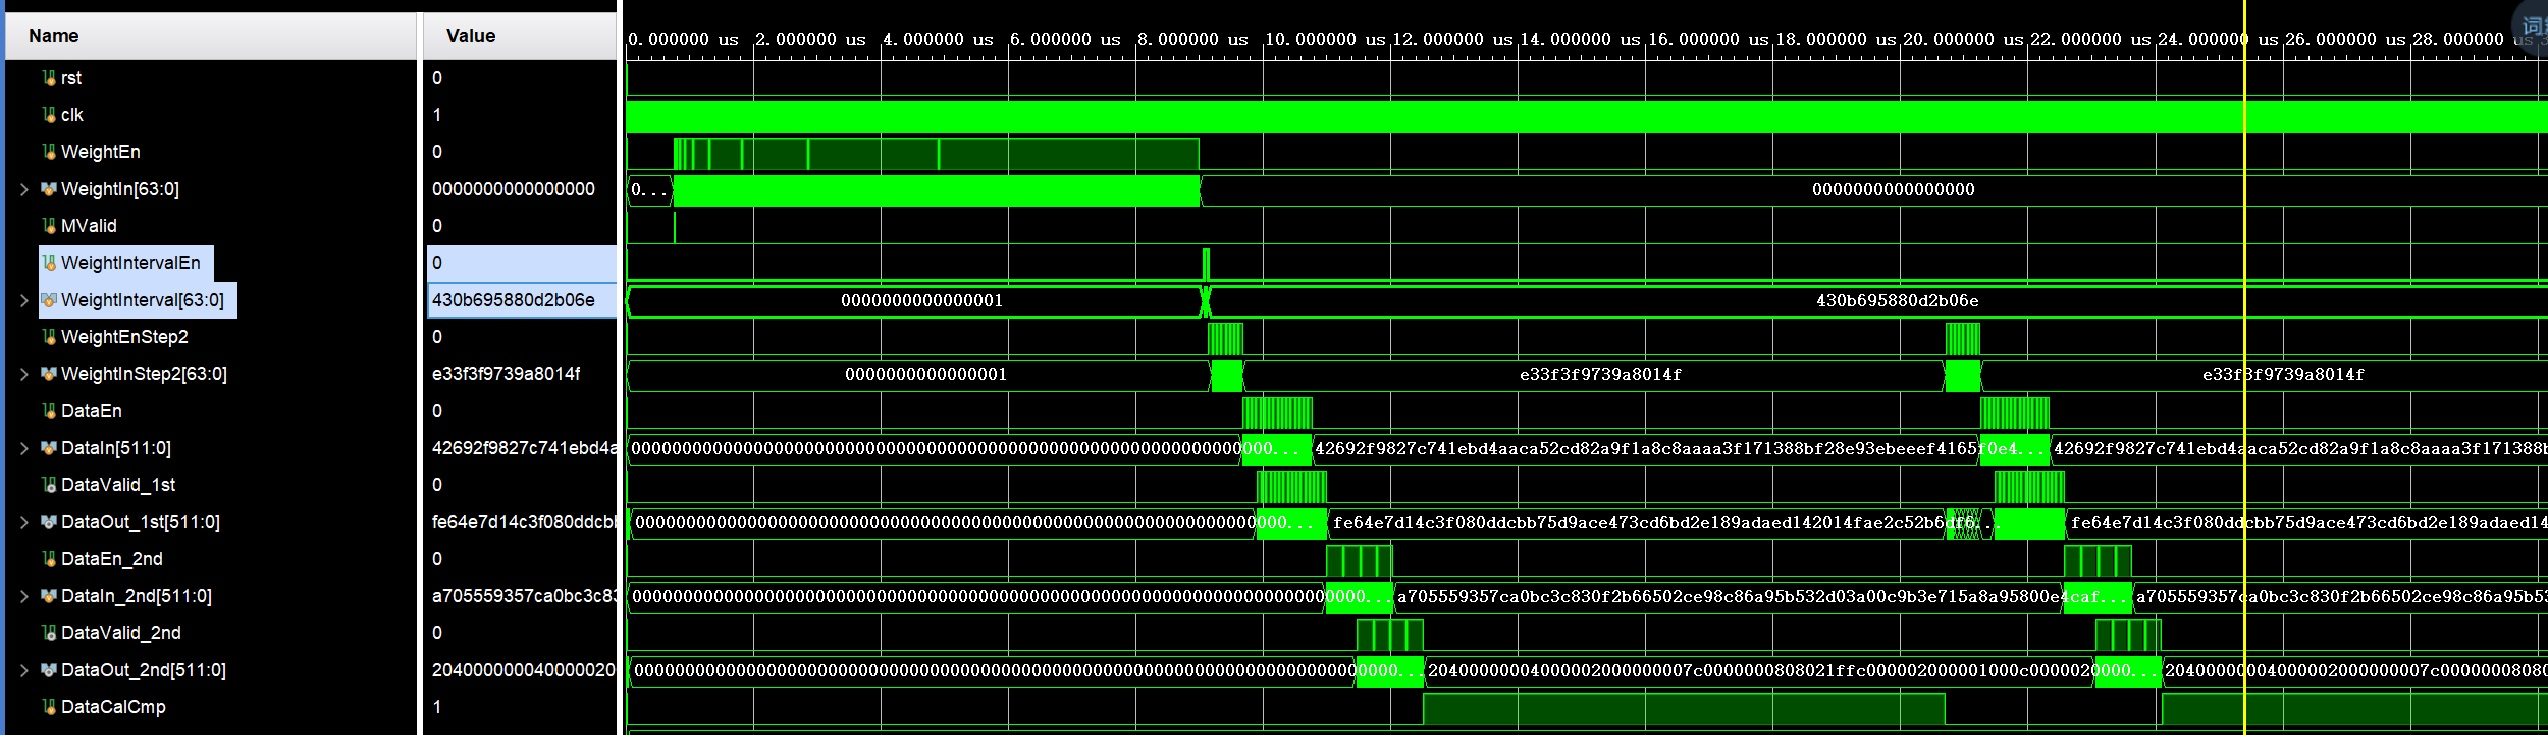
\includegraphics[width=1\textwidth]{NTT simulation.jpg}
  \caption{NTT simulation}
  \label{fig:NTT_Simu}
\end{figure}

In the Figure: the signals of WeightEn and WeightIn are the configurations for the twiddle factors of the NTT module; WeightEnStep2 and WeightInStep2 are twiddle factors for the output of large number modular multiplication in the NTT module; signals of WeightIntervalEn and WeightIntervalIn are used to be accumulated twiddle factors when updating the twiddle to multiply the outputs of NTT blocks; DataIn and DataEn are the input data for the first dimension of the NTT, while DataOut\_1st and DataValid\_1st are the computed results outputted; DataIn\_2nd and DataEn\_2nd are the input data for the second dimension of the NTT, and DataOut\_2nd and DataValid\_2nd are the computed results outputted; DataCalCmp is used for indicate the comparison of the computed NTT results with the theoretical ones.

In the implementation, 8-way parallel NTT acceleration is used. According to the timing, the NTT engine is respectively configured with LUT twiddle factors, LUT twiddle factors of modular multiplication, and accumulated twiddle factors. To compute a 4096-point NTT, the size of the 2D array is 8 * 16 * 32 for the first passs and 8 * 4 * 128 for the second one. Based on the comparison signal DataCalCmp, the results obtained from the 2D NTT operation are consistent with the theoretical values. When performing the second 4096-point NTT acceleration, it is only necessary to reload the modular multiplication LUT twiddle factors.
